\documentclass[12pt]{article}
\usepackage{makecell}
\usepackage{hyphenat}
\usepackage[utf8]{vietnam}
% Removed hyphsubst to fix compilation error
% \usepackage[vietnamese=nohyphenation]{hyphsubst}
\usepackage[vietnamese]{babel}
\usepackage[dvipsnames]{xcolor}
\usepackage{booktabs} % Required for nicer horizontal lines
\usepackage{ragged2e}
\usepackage{caption}
\usepackage{subcaption}
\usepackage{float}
\usepackage{amsmath,amssymb,amsfonts}
\usepackage{graphicx}
\usepackage{adjustbox}
\usepackage{multicol}
\usepackage[inline,shortlabels]{enumitem}
\usepackage{setspace}
\usepackage{longtable}
\usepackage{bm} 
\usepackage[inkscapelatex=false]{svg}
\usepackage{titling}
\usepackage{tabularx}
\usepackage[T1]{fontenc}
\usepackage{lmodern,mathrsfs}
% \usepackage[draft]{hyperref}
\usepackage{hyperref}
\usepackage{xparse}
\usepackage{fontawesome5}
\usepackage[most]{tcolorbox}
\usepackage{tikz}
\usepackage[framemethod=TikZ]{mdframed}
\usetikzlibrary{matrix, fit, shadows, positioning, arrows.meta, calc, shapes.geometric, backgrounds, shapes.symbols}
\usepackage{paracol}
\usepackage{bbm}
\usepackage{pgfplots}
\usepackage{siunitx}
\usepackage{multirow}
%  biblatex (thay cho IEEEtran.bst) ------------------------------------
\usepackage[
    backend=bibtex,
    style=ieee,
    citestyle=numeric-comp,
    maxnames=1,     % chỉ hiển thị 1 tên tác giả, phần còn lại thành ``et al."
    minnames=1,
    uniquelist=false,
    hyperref=false
]{biblatex}
\usepackage{forest}
\addbibresource{references.bib}
\DefineBibliographyStrings{english}{
  andothers = {et\addabbrvspace al\adddot}
}
\AtBeginBibliography{\selectlanguage{english}}

% -----------------------------------------------------------------
\AtBeginDocument{\renewcommand\refname{}}

\usepackage[toc,page]{appendix}
\renewcommand{\appendixtocname}{Phụ lục}      
\renewcommand{\appendixpagename}{Phụ lục}

\usepackage{xurl}
\setlength{\headheight}{14.5pt}
\setlength{\topmargin}{-.5in} \setlength{\textheight}{9.25in}
\setlength{\oddsidemargin}{-0.1in} \setlength{\textwidth}{6.8in}

\usepackage{tocloft}
\renewcommand{\cfttoctitlefont}{\Huge\bfseries}
\setlength{\cftaftertoctitleskip}{2em}
\setlength{\cftbeforesubsecskip}{7pt} % giãn cách subitem mục lục
\renewcommand{\cftsecleader}{\cftdotfill{\cftdotsep}}
\setlength{\cftsecnumwidth}{3em}
\renewcommand{\cftsecaftersnum}{\quad}
\renewcommand{\cftsubsecleader}{\cftdotfill{\cftdotsep}}
\setlength{\cftsubsecnumwidth}{4em}
\renewcommand{\cftsubsecaftersnum}{\quad}
\renewcommand{\cftsubsubsecleader}{\cftdotfill{\cftdotsep}}
\setlength   {\cftsubsubsecnumwidth}{5em}  
\renewcommand{\cftsubsubsecaftersnum}{\quad}

\PassOptionsToPackage{vietnamese.licr}{babel}
\usepackage{vipythonhighlight}
\usepackage{tvietlistings}
\newcounter{mycounter}
\newcommand\showmycounter{\stepcounter{mycounter}\themycounter}
\usepackage{lipsum}
\newcommand\showlips{\stepcounter{mycounter}\lipsum[\value{mycounter}]}

%--------------------------------------------------------------------
\usepackage{framed}
\usepackage{fancyhdr}
\usepackage{upquote}
\usepackage{listings}	 
	    

\usepackage[toc, nonumberlist, style=super]{glossaries}
\makenoidxglossaries

\newglossarystyle{clean3col}{%
    % 1) Table layout: 3 columns
    \renewenvironment{theglossary}%
    {%
      \begin{longtable}{@{}
        >{\setlength{\parindent}{0pt}\RaggedRight\arraybackslash}p{0.2\linewidth}
        >{\setlength{\parindent}{0pt}\RaggedRight\arraybackslash}p{0.23\linewidth}
        >{\setlength{\parindent}{0pt}\RaggedRight\arraybackslash}p{0.52\linewidth}
      @{}}%
    }%
    {\end{longtable}}%

    % 2) Header row
    \renewcommand{\glossaryheader}{%
        \bfseries Thuật ngữ &
        \bfseries Tạm dịch &
        \bfseries Mô tả \\
        \midrule
        \endhead
    }%

    % 3) Each entry row
    \renewcommand{\glossentry}[2]{%
        \itshape \glstarget{##1}{\glossentryname{##1}} &
        \glsentryuseri{##1} &
        \glossentrydesc{##1} \\
        \addlinespace[6pt]
    }%
}


% Color --------------------------------------------------------------------
\usepackage{epigraph}
\usepackage{titlesec}

\definecolor{codebackground}{RGB}{250, 250, 250}
\definecolor{codecomment}{RGB}{34, 139, 34}
\definecolor{codekeyword}{RGB}{0, 0, 255}
\definecolor{codestring}{RGB}{255, 0, 0}
\definecolor{codeidentifier}{RGB}{0, 0, 0}
\definecolor{codelinenumbers}{RGB}{90, 90, 90}

\definecolor{codegreen}{rgb}{0,0.6,0}
\definecolor{codegray}{rgb}{0.5,0.5,0.5}
\definecolor{codepurple}{rgb}{0.58,0,0.82}
\definecolor{backcolour}{rgb}{0.95,0.95,0.92}

\definecolor{aivnGreen}{RGB}{52,79,30}  
\definecolor{aivnCodeOutputColor}{RGB}{11,83,148}  
\definecolor{captiongray}{gray}{0.15} 
\definecolor{captionbg}{RGB}{250,250,250}

\definecolor{foldercolor}{RGB}{0, 102, 204}
\definecolor{filecolor}{RGB}{104, 104, 104}
\definecolor{scriptcolor}{RGB}{180, 50, 50}
\definecolor{pythoncolor}{RGB}{0, 128, 128}

% --- Extra Brand colors for the table ---
\definecolor{brandIndigo}{HTML}{333D91} 
\definecolor{rowLavender}{HTML}{EEECFA}
\setlength{\parskip}{0.3em}

% Table
\newtcolorbox{captionbelowboxaivn}{
    colback=aivnGreen,
    colframe=aivnGreen,
    boxrule=0pt,
    arc=4pt,
    left=4pt,
    right=4pt,
    top=2pt,
    bottom=2pt,
    width=\linewidth,
    boxsep=4pt,
    halign=center,
    % fontupper=\bfseries\color{white}
    fontupper=\color{white}
}

% Figure
\newtcolorbox{figurecardcaptionaivn}{
  colback=aivnGreen,        % Màu nền (background color)
  colframe=aivnGreen,       % Màu viền box (border color)
  boxrule=0pt,              % Độ dày viền box (0pt = không viền)
  arc=2pt,                  % Độ bo góc (2pt là bo nhẹ, tăng để bo tròn hơn)
  top=3pt,                  % Padding phía trên nội dung
  bottom=3pt,               % Padding phía dưới nội dung
  left=10pt,                % Padding bên trái
  right=10pt,               % Padding bên phải
  width=\linewidth,         % Chiều rộng bằng toàn bộ dòng
  fontupper=\small\fontsize{11pt}{13pt}\selectfont\color{white} 
}

% Tạo counter riêng
\newcounter{hinh}
% Định nghĩa macro caption Hình
\newcommand{\capfig}[1]{%
  \refstepcounter{hinh}%
  % \textbf{Hình~\thehinh:}~#1
    Hình~\thehinh:~#1
}

\newtcolorbox{figurecaptionmodern}{
  colback=captionbg,
  colframe=aivnGreen,
  boxrule=1.5pt,
  bottomrule=2pt,  
  toptitle=0pt,
  bottomtitle=0pt,
  left=6pt,
  right=6pt,
  top=4pt,
  bottom=2pt,
  width=\linewidth,
  fontupper=\small\fontsize{11pt}{13pt}\selectfont\color{black},
  halign=center
}

% Code Block -----------------------------------------------------------------
\newtcolorbox{aivncodebox}[1][]{%
  enhanced,
  colback=gray!10,
  colframe=aivnGreen,
  coltitle=white,
  colbacktitle=aivnGreen,
  title=#1,
  fonttitle=\bfseries\sffamily,
  listing only,
  breakable,
  listing engine=listings,
  listing options={
    language=Python,
    basicstyle=\ttfamily\footnotesize,
    commentstyle=\color{ForestGreen},
    keywordstyle=\color{blue},
    stringstyle=\color{red!70!black},
    numbers=left, upquote=true,
    numberstyle=\tiny\color{gray},
    numbersep=5pt,
    breaklines=true,
    showstringspaces=false,
    xleftmargin=1.5em,
    framexleftmargin=1.5em
  }
}

% Code Output Block -----------------------------------------------------------------
\newtcolorbox{aivnCodeOutput}[1][]{%
  enhanced,
  colback=gray!10,
  colframe=aivnCodeOutputColor,
  coltitle=white,
  colbacktitle=aivnCodeOutputColor,
  title=#1,
  fonttitle=\bfseries\sffamily,
  listing only,
  breakable,
  listing engine=listings,
  listing options={
    language=Python,
    basicstyle=\ttfamily\footnotesize,
    commentstyle=\color{ForestGreen},
    keywordstyle=\color{blue},
    stringstyle=\color{red!70!black},
    numbers=left,
    numberstyle=\tiny\color{gray},
    numbersep=5pt,
    breaklines=true,
    showstringspaces=false,
    xleftmargin=1.5em,
    framexleftmargin=1.5em
  }
}

% Last argument allows more tcolorbox options to be added

% --- Guideline/Tip box ---
\newtcolorbox{guidelinebox}[2][]{
    enhanced, colback=yellow!10!white, colframe=orange!90!black, boxrule=1pt, arc=4pt,
    fonttitle=\bfseries, attach boxed title to top left={yshift=-2mm, xshift=3mm},
    colbacktitle=orange!90!black, coltitle=white,
    title=\faLightbulb\hspace{1mm} #2, #1
}

\newtcolorbox{notebox}[1][]{
  enhanced,  colback=yellow!10, colframe=orange!80, boxrule=1pt, 
  arc=4pt, fontupper=\small, attach boxed title to top left={yshift=-2mm, xshift=3mm},
  colbacktitle=orange!80,  coltitle=white, fonttitle=\bfseries,  
  title=\faInfoCircle~\textbf{Lưu ý},  #1
}

\newtcolorbox{infobox}[1]{%
    enhanced, 
    breakable, 
    colback=green!3, 
    colframe=green!3, 
    arc=5pt,
    borderline west={3pt}{0pt}{aivnGreen},
    attach boxed title to top left={ 
        yshift*=-\tcboxedtitleheight/2, 
        xshift=-0.1em 
    },
    colbacktitle=aivnGreen, %
    coltitle=white, 
    fonttitle=\bfseries, 
    boxed title style={ 
        arc=4pt, 
        top=2pt, 
        bottom=2pt,
        left=8pt,
        right=8pt,
    },
    title={\faInfoCircle\quad #1}
}
\newtcolorbox{examplebox}[1]{%
    enhanced,
    breakable,
    colback=brandIndigo!5,      
    colframe=brandIndigo!5,     
    arc=5pt,
    borderline west={3pt}{0pt}{brandIndigo}, 
    attach boxed title to top left={
        yshift*=-\tcboxedtitleheight/2,
        xshift=-0.1em
    },
    colbacktitle=brandIndigo,   
    coltitle=white,
    fonttitle=\bfseries,
    boxed title style={
        arc=4pt,
        top=2pt,
        bottom=2pt,
        left=8pt,
        right=8pt,
    },
    title={\faLightbulb\quad #1} 
}
% Prompt Block ---------------------------------------------------------------
\definecolor{promptBlue}{HTML}{2F5D8C}
\definecolor{promptBg}{HTML}{F6F9FC}
\definecolor{promptBorder}{HTML}{B7C9DC}

% Dùng cho prompt đã viết theo cú pháp LaTeX bình thường
\newtcolorbox{promptbox}[1][Prompt]{%
    enhanced,
    breakable,
    colback=promptBg,
    colframe=promptBorder,
    coltitle=white,
    colbacktitle=promptBlue,
    fonttitle=\bfseries\sffamily,
    title={#1},
    boxrule=0.8pt,
    arc=4pt,
    left=8pt,
    right=8pt,
    top=2pt,
    bottom=1pt,
    before skip=8pt,
    after skip=8pt,
    borderline west={3pt}{0pt}{promptBlue},
    fontupper=\small\sffamily,
}

% Dùng cho prompt raw: giữ nguyên xuống dòng, không highlight keyword
\newtcblisting{promptboxraw}[1][Prompt]{%
    enhanced,
    breakable,
    listing only,
    listing engine=listings,
    colback=promptBg,
    colframe=promptBorder,
    coltitle=white,
    colbacktitle=promptBlue,
    fonttitle=\bfseries\sffamily,
    title={#1},
    boxrule=0.8pt,
    arc=4pt,
    left=8pt,
    right=8pt,
    top=-4pt,
    bottom=-4pt,
    before skip=4pt,
    after skip=4pt,
    borderline west={3pt}{0pt}{promptBlue},
    listing options={
        language={},
        basicstyle=\small\ttfamily,
        columns=fullflexible,
        keepspaces=true,
        breaklines=true,
        showstringspaces=false,
        numbers=none,
        frame=none,
        keywordstyle=\color{black},
        commentstyle=\color{black},
        stringstyle=\color{black},
        identifierstyle=\color{black}
    }
}


%--------------------------------------------------------------------
\lstdefinestyle{mystyle}{
    backgroundcolor=\color{codebackground},
    commentstyle=\color{codecomment},
    keywordstyle=\color{codekeyword},
    stringstyle=\color{codestring},
    identifierstyle=\color{codeidentifier},
    basicstyle=\ttfamily\footnotesize,
    breakatwhitespace=false,
    breaklines=true,
    captionpos=b,
    keepspaces=true,
    numbers=left,
    numberstyle=\tiny\color{codelinenumbers}, 
    numbersep=5pt,
    showspaces=false,
    showstringspaces=false,
    showtabs=false,
    tabsize=2
}

\lstset{style=mystyle}

\hypersetup{
    colorlinks=true,
    linkcolor=black,
    filecolor=magenta,    
    citecolor=green,
    urlcolor=blue,
    pdftitle={Overleaf Example},
    pdfpagemode=FullScreen,
}

%--------------------------------------------------------------------
\newcounter{choice}
\renewcommand\thechoice{($\alph{choice}$)}
\newcommand\choicelabel{\thechoice}

%--------------------------------------------------------------------
\newenvironment{choices}%
  {\list{\choicelabel}%
     {\usecounter{choice}\def\makelabel##1{\hss\llap{##1}}%
       \settowidth{\leftmargin}{W.\hskip\labelsep\hskip 0 em}%
       \def\choice{%
         \item
       } % choice
       \labelwidth\leftmargin\advance\labelwidth-\labelsep
       \topsep=0pt
       \partopsep=0pt
     }%
  }%
  {\endlist}
  
%--------------------------------------------------------------------
\def\CChoice{%
      \choice
      \addanswer{\theenumi}{\thechoice}%
    }
    \let\CChoice\CChoice
%    \par % Uncomment this to have choices always start a new line
   % \let\par\@empty
    % If we're continuing the textbf containing the question,
    % then leave a bit of space before the first choice:
    \ifvmode\else\enskip\fi
    \ignorespaces
  %
  {}
\makeatother
\newbox\allanswers
\setbox\allanswers=\hbox{}
\newcommand{\addanswer}[2]{%
  \global\setbox\allanswers=\hbox{\unhbox\allanswers \quad #1.~#2}%
}
\newcommand{\showanswers}{%
  \vfill
  \begin{center}
    Answers
  \end{center}
  \unhbox\allanswers
}

\makeatletter
\newenvironment{multichoices}[1][1]{%
\begin{multicols}{#1}}{%
\end{multicols}}
\makeatother

\pagestyle{fancy}

\DeclareMathOperator*{\argmax}{arg\,max}
\DeclareMathOperator*{\argmin}{arg\,min}
\DeclareMathOperator{\E}{\mathbb{E}}

% Outline --------------------------------------------------------------------
% Section numbering ----------------------------------------------------------
\renewcommand{\thesection}{\Roman{section}.} 
\renewcommand{\thesubsection}{\thesection\arabic{subsection}.}
\renewcommand{\thesubsubsection}{\thesubsection\arabic{subsubsection}.}

% Paper-like section title sizes --------------------------------------------
% Title paper: 17pt
% Section should be clearly smaller than title but still prominent.
\titleformat{\section}
  {\normalfont\fontsize{16pt}{20pt}\selectfont\bfseries}
  {\thesection}
  {0.85em}
  {}

\titleformat{\subsection}
  {\normalfont\fontsize{14pt}{16pt}\selectfont\bfseries}
  {\thesubsection}
  {0.75em}
  {}

\titleformat{\subsubsection}
  {\normalfont\fontsize{12pt}{15pt}\selectfont\bfseries}
  {\thesubsubsection}
  {0.65em}
  {}

% Paper-like compact spacing -------------------------------------------------
\titlespacing*{\section}
  {0pt}
  {1.25em plus 0.2em minus 0.1em}
  {0.65em plus 0.1em minus 0.1em}

\titlespacing*{\subsection}
  {0pt}
  {1.0em plus 0.2em minus 0.1em}
  {0.45em plus 0.1em minus 0.1em}

\titlespacing*{\subsubsection}
  {0pt}
  {0.85em plus 0.15em minus 0.1em}
  {0.35em plus 0.1em minus 0.1em}


% Logo + Title ---------------------------------------------------------------

\setlength{\droptitle}{-7em}

% Title horizontal rule
\newcommand{\TitleRule}{%
  \rule{0.90\textwidth}{0.6pt}
}

% Chiều cao vùng title giữa 2 rule
\newlength{\TitleBlockHeight}
\setlength{\TitleBlockHeight}{2.2cm}

\pretitle{%
  

  % Logo row removed

  %\vspace{0.2em}

\begin{center}
  \TitleRule
  \par\nointerlineskip
}

\title{%
  \parbox[c][\TitleBlockHeight][c]{0.90\textwidth}{%
    \centering
    {\fontsize{18pt}{22pt}\selectfont\bfseries Hệ thống RAG học tập cá nhân hóa dựa trên tài liệu}
  }%
}

\posttitle{%
  \par\nointerlineskip
  \TitleRule
  \end{center}
}

\preauthor{%
  \begin{center}
  \fontsize{11pt}{13pt}\selectfont
}

\author{%
  \textbf{DAT301m AI1911 TEAM 3}\\
  \vspace{1em}
  \textbf{Trần Công Cường - HE187231} \hspace{2.8em} \textbf{Nguyễn Anh Quân - HE194919}\\
  \vspace{1em}
  \textbf{Trần Quốc Đạt - HE194073 } \hspace{2.8em} \textbf{Võ Nhật Minh - HE195010}
}

\postauthor{%
  \par
  \end{center}
}

\date{}
% Header --------------------------------------------------------------------
\pagestyle{fancy}
\fancyhf{}
\lhead{}
\rhead{}
\fancyfoot[c]{\thepage}
\renewcommand{\headrulewidth}{0pt}

\renewcommand{\footrulewidth}{1.0pt}
\renewcommand{\footrule}{%
    {\color{aivnGreen}\hrule width\headwidth height\footrulewidth}
}


\fancypagestyle{firstpage}{
    \fancyhf{}
    \fancyfoot[c]{\thepage}
    \renewcommand{\headrulewidth}{0pt}
    \renewcommand{\footrulewidth}{1.0pt}
    \renewcommand{\footrule}{%
        {\color{aivnGreen}\hrule width\headwidth height\footrulewidth}
    }
}


\begin{document}
\maketitle
\thispagestyle{firstpage}
\vspace{-3em}

\begin{abstract}
\noindent Mô hình ngôn ngữ lớn (LLM) đã mở ra nhiều ứng dụng tiềm năng trong giáo dục. Tuy nhiên, tình trạng sinh thông tin sai lệch (hallucination) làm hạn chế độ tin cậy của chúng. Dự án này xây dựng một hệ thống học tập cá nhân hóa dựa trên tài liệu PDF, đóng vai trò như một phiên bản NotebookLM thu gọn. Hệ thống áp dụng kiến trúc Retrieval-Augmented Generation (RAG) kết hợp với các kỹ thuật tiền xử lý văn bản, lưu trữ vector và truy xuất ngữ nghĩa để đảm bảo mô hình ngôn ngữ sinh ra các câu trả lời chính xác, bám sát nội dung gốc. Báo cáo này trình bày toàn bộ quá trình xây dựng hệ thống, từ kiến trúc tổng thể, pipeline xử lý dữ liệu, cơ chế truy xuất, cho đến việc tích hợp các tính năng học tập (tóm tắt, tạo câu hỏi trắc nghiệm, flashcards) và cuối cùng là đánh giá hiệu suất mô hình bằng framework Ragas.
\end{abstract}

\section{Giới thiệu}
Các mô hình ngôn ngữ lớn (LLM) đang được ứng dụng rộng rãi trong học tập, nghiên cứu và khai thác tri thức từ tài liệu. Tuy nhiên, khi áp dụng vào các bài toán giáo dục, tính chính xác, khả năng kiểm chứng và mức độ bám sát tài liệu nguồn là những yêu cầu vô cùng quan trọng. Nếu chỉ dựa vào tri thức nội tại, LLM có thể sinh ra thông tin sai lệch hoặc không có căn cứ (hallucination).

Dự án này mô phỏng một hệ thống hỗ trợ học tập dựa trên tài liệu cá nhân, lấy cảm hứng từ ứng dụng NotebookLM của Google. Thay vì để LLM trả lời tự do, hệ thống sử dụng kiến trúc Retrieval-Augmented Generation (RAG) để truy xuất các đoạn nội dung liên quan từ tài liệu đã được nạp trước, sau đó đưa ngữ cảnh này vào \textit{prompt} để sinh phản hồi. Báo cáo này trình bày chi tiết về toàn bộ quá trình xây dựng và đánh giá hệ thống, bao gồm kiến trúc lõi, các module chức năng và các bước thực nghiệm tối ưu hóa hiệu suất truy xuất.

\section{Nghiên cứu liên quan}

Hệ thống hỗ trợ học tập cá nhân hóa dựa trên tài liệu chuyên ngành nằm ở giao điểm liên ngành của nhiều hướng nghiên cứu cốt lõi trong Xử lý Ngôn ngữ Tự nhiên (NLP), Hệ thống Thông tin (IR) và Khoa học Nhận thức trong Giáo dục (Cognitive Science in Education): kiến trúc Tạo sinh Tăng cường Truy xuất (RAG), biểu diễn ngữ nghĩa mật và tái xếp hạng đa tầng, cơ chế khử ảo giác và tạo sinh kèm trích dẫn có thể kiểm chứng, mô hình hóa tài liệu dài thông qua tóm tắt phân cấp, các phương pháp sư phạm gợi nhớ chủ động (Active Recall), cùng phương pháp luận đánh giá tự động dựa trên LLM. Phần này phân tích có hệ thống các công trình nền tảng và cập nhật nhất, chỉ ra các khoảng trống công nghệ hiện hữu và định vị đóng góp học thuật của hệ thống đề xuất.

\subsection{Sự tiến hóa của kiến trúc RAG và Các điểm nghẽn kỹ thuật thực tiễn}
Khái niệm Tạo sinh Tăng cường Truy xuất (\textit{Retrieval-Augmented Generation} -- RAG) được khởi xướng bởi Lewis et al. \cite{lewis2020retrieval} nhằm khắc phục hai hạn chế cố hữu của các mô hình ngôn ngữ lớn (LLM): tri thức tham số tĩnh (\textit{static parametric memory}) bị lỗi thời theo thời gian và xu hướng suy luận sai lệch khi đối mặt với các miền tri thức chuyên sâu hoặc tài liệu nội bộ. Trong khảo sát tổng quan hệ thống, Gao et al. \cite{gao2023rag_survey} đã phân loại tiến trình tiến hóa của RAG thành ba thế hệ kiến trúc tiêu biểu:
\begin{enumerate}
    \item \textbf{Naive RAG:} Hoạt động theo quy trình tuần tự tuyến tính giản đơn gồm ba bước: phân đoạn tài liệu (\textit{chunking}), nhúng vector lưu vào cơ sở dữ liệu, và truy xuất $K$ đoạn văn bản có độ tương đồng cosine cao nhất để ghép trực tiếp vào prompt tạo sinh. Mặc dù dễ cài đặt, Naive RAG thường bộc lộ sự suy giảm hiệu năng nghiêm trọng do không có cơ chế lọc nhiễu và tinh chế ngữ cảnh.
    \item \textbf{Advanced RAG:} Bổ sung các kỹ thuật tối ưu hóa trước truy xuất (\textit{pre-retrieval}) như phân đoạn đa mức, bóc tách cấu trúc tài liệu; đồng thời tích hợp giai đoạn sau truy xuất (\textit{post-retrieval}) gồm nén ngữ cảnh và tái xếp hạng chuyên sâu (\textit{reranking}) để tối đa hóa tính liên quan của dữ liệu nạp vào LLM.
    \item \textbf{Modular RAG:} Mở rộng kiến trúc thành các module linh hoạt có thể định tuyến động (\textit{dynamic routing}), lặp lại truy xuất (\textit{iterative retrieval}) hoặc kết hợp tìm kiếm đồ thị tri thức (\textit{knowledge graph}).
\end{enumerate}

Mặc dù các mô hình lý thuyết phát triển nhanh chóng, việc triển khai RAG trong các ứng dụng thực tế thường đối mặt với các thách thức kỹ thuật phức tạp. Trong nghiên cứu phân tích lỗi thực nghiệm toàn diện, Barnett et al. \cite{barnett2024seven_failures} đã định danh \textbf{7 điểm lỗi kỹ thuật điển hình} (\textit{Seven Failure Points}) làm tê liệt hệ thống RAG trong thực tế:
\begin{itemize}
    \item \textit{FP1 -- Missing Content:} Tài liệu nạp vào không chứa thông tin hoặc parser không trích xuất được do định dạng phức tạp.
    \item \textit{FP2 -- Missed Top Ranked:} Đoạn văn bản chứa câu trả lời đúng bị bỏ sót trong top-$K$ ban đầu do hạn chế của giải thuật nhúng vector.
    \item \textit{FP3 -- Not in Context:} Đoạn văn bản đúng bị loại bỏ trong quá trình tinh lọc hoặc cắt cụt ngữ cảnh.
    \item \textit{FP4 -- Not Extracted:} LLM không trích xuất được thông tin dù dữ kiện đã có sẵn trong ngữ cảnh do hiện tượng bão hòa chú ý.
    \item \textit{FP5 -- Wrong Format:} LLM vi phạm cấu trúc định dạng đầu ra (ví dụ sinh JSON lỗi cú pháp khi tạo câu hỏi trắc nghiệm).
    \item \textit{FP6 -- Incorrect Specificity:} Phản hồi quá chung chung hoặc quá chi tiết, không giải quyết đúng trọng tâm của người dùng.
    \item \textit{FP7 -- Incomplete:} Câu trả lời chỉ phản ánh một phần dữ kiện do ngữ cảnh bị phân mảnh qua nhiều đoạn văn bản khác nhau.
\end{itemize}

\noindent \textbf{Định vị đóng góp:} Hệ thống của chúng tôi được xây dựng theo chuẩn \textbf{Advanced RAG}, giải quyết trực diện 7 điểm lỗi trên thông qua: cơ chế nạp đa định dạng kèm băm SHA-1 định danh tệp (khắc phục FP1), pipeline truy xuất hai tầng kết hợp Bi-Encoder và Cross-Encoder (khắc phục FP2, FP3, FP4), khuôn mẫu prompt ràng buộc trích dẫn mịn $[S_i]$ (khắc phục FP6, FP7), và cơ chế kiểm định phòng vệ hai lớp (\textit{Two-Tier Defensive Validation}) với Pydantic nhằm triệt tiêu hoàn toàn lỗi sai cấu trúc đầu ra (khắc phục triệt để FP5).

\subsection{Biểu diễn ngữ nghĩa Bi-Encoder và Tái xếp hạng chuyên sâu bằng Cross-Encoder}
Trong bài toán tìm kiếm ngữ nghĩa, phương pháp Dense Passage Retrieval (DPR) \cite{karpukhin2020dense} đã chứng minh tính ưu việt vượt bậc so với các giải thuật so khớp từ khóa cổ điển (như BM25 hay TF-IDF) nhờ khả năng nắm bắt ngữ nghĩa tiềm ẩn trong không gian vector liên tục. Bước tiến gần đây của Wang et al. \cite{wang2024e5} với mô hình Multilingual-E5 (\texttt{intfloat/multilingual-e5-large}) đã tối ưu hóa không gian vector đa ngôn ngữ thông qua kỹ thuật học tương phản phi giám sát (\textit{weakly-supervised contrastive pre-training}) trên quy mô dữ liệu khổng lồ với hàm mất mát InfoNCE:
\begin{equation}
    \mathcal{L}_{\text{contrastive}} = - \log \frac{\exp\left(\cos(\mathbf{e}_q, \mathbf{e}_{d^+}) / \tau\right)}{\exp\left(\cos(\mathbf{e}_q, \mathbf{e}_{d^+}) / \tau\right) + \sum_{j=1}^{M} \exp\left(\cos(\mathbf{e}_q, \mathbf{e}_{d^-_j}) / \tau\right)}
\end{equation}
trong đó $\mathbf{e}_q, \mathbf{e}_d \in \mathbb{R}^{1024}$ lần lượt là vector nhúng của câu truy vấn và đoạn văn bản, được phân định bằng tiền tố tác vụ bất đối xứng (\texttt{"query: "} và \texttt{"passage: "}), và $\tau$ là tham số nhiệt độ (\textit{temperature}). Nhờ cơ chế tách biệt không gian biểu diễn (Bi-Encoder), toàn bộ kho tài liệu có thể được vector hóa ngoại tuyến và lưu trữ trong cơ sở dữ liệu vector Qdrant, cho phép tìm kiếm láng giềng gần nhất xấp xỉ (\textit{Approximate Nearest Neighbor} -- ANN) dựa trên đồ thị HNSW với độ phức tạp truy vấn $O(\log N)$ hoặc xấp xỉ $O(1)$.

Tuy nhiên, kiến trúc Bi-Encoder tồn tại hai hạn chế lý thuyết và thực nghiệm cốt tử:
\begin{enumerate}
    \item \textbf{Nút thắt cổ chai biểu diễn (\textit{Representation Bottleneck}):} Việc nén toàn bộ thông tin phong phú của một đoạn văn bản $L$ token thành một vector độc lập duy nhất làm mất đi hoàn toàn các tương tác tương hỗ tinh tế giữa các từ trong câu hỏi và văn bản (\textit{late interaction loss}).
    \item \textbf{Hiện tượng suy giảm chú ý ở đoạn giữa (\textit{"Lost in the Middle"}):} Nghiên cứu thực nghiệm đột phá của Liu et al. \cite{liu2023lost} chứng minh rằng các mô hình ngôn ngữ dựa trên Transformer thể hiện đường cong hiệu năng dạng chữ U: khả năng truy xuất và suy luận đạt đỉnh ở đầu và cuối chuỗi ngữ cảnh, nhưng suy giảm nghiêm trọng đối với các đoạn văn bản nằm ở khoảng giữa (chiếm 60\% chiều dài prompt). Do đó, việc nhồi nhét một danh sách dài các chunk từ Bi-Encoder vào prompt sẽ phản tác dụng, trực tiếp kích hoạt hiện tượng ảo giác.
\end{enumerate}

Để dung hòa mâu thuẫn giữa tốc độ tính toán và độ chính xác ngữ cảnh, các nghiên cứu tiên phong của Xiao et al. \cite{xiao2023c} và Chen et al. \cite{chen2024bge_m3} đã giới thiệu kiến trúc Cross-Encoder tái xếp hạng chuyên sâu (\texttt{BAAI/bge-reranker-v2-m3}). Khác với Bi-Encoder, Cross-Encoder ghép nối trực tiếp chuỗi token của câu hỏi và đoạn văn bản vào cùng một mạng Transformer duy nhất để tính toán ma trận chú ý tương hỗ toàn phần (\textit{Full Cross-Attention}) trên từng cặp token:
\begin{equation}
    s(q, d) = \sigma\left(\mathbf{w}^\top \text{Transformer}(\text{[CLS]} \circ q \circ \text{[SEP]} \circ d)\right)
\end{equation}
Mặc dù phép tính chú ý toàn phần có độ phức tạp tính toán bậc hai $\mathcal{O}((|q| + |d|)^2)$ khiến Cross-Encoder không thể áp dụng trực tiếp trên toàn bộ cơ sở dữ liệu hàng triệu vector, nó lại cực kỳ hiệu quả khi đóng vai trò bộ lọc tinh chế trên một tập ứng viên thu nhỏ.

\noindent \textbf{Định vị đóng góp:} Hệ thống của chúng tôi hiện thực hóa cơ chế \textbf{Truy xuất hai tầng (Two-Stage Retrieval)} phối hợp đạt điểm tối ưu Pareto:
\begin{itemize}
    \item \textbf{Tầng 1 (Coarse Retrieval):} Sử dụng Multilingual-E5-large kết hợp chỉ mục HNSW trong Qdrant mở rộng biên độ thu hồi $K_{\text{initial}} = 15$ chunks với độ trễ thấp, đảm bảo độ bao phủ (Recall) tối đa và loại bỏ nguy cơ bỏ sót thông tin (FP2).
    \item \textbf{Tầng 2 (Fine Reranking):} Sử dụng BGE-Reranker-v2-m3 thực hiện phân tích tương tác sâu, tái thẩm định và cô đọng thành top $K_{\text{rerank}} = 5$ chunks có điểm số tương quan cao nhất. Quy trình này vừa triệt tiêu hiện tượng \textit{"Lost in the Middle"}, vừa giảm thiểu 66.7\% ngân sách token nạp vào LLM, giúp tăng độ chính xác phản hồi và rút ngắn thời gian sinh.
\end{itemize}

\subsection{Khử ảo giác và Sinh văn bản kèm trích dẫn có thể kiểm chứng}
Hiện tượng ảo giác (\textit{hallucination}) --- mô hình tự sinh các dữ kiện không có thực hoặc suy luận sai lệch logic với phong cách hành văn hết sức thuyết phục --- là rào cản lớn nhất khi ứng dụng LLM vào môi trường giáo dục và nghiên cứu học thuật \cite{ji2023survey}. Trong bối cảnh sư phạm, thông tin sai lệch từ AI có thể trực tiếp làm sai lệch nhận thức của người học, gây ra những hệ quả nghiêm trọng.

Nhằm giải quyết bài toán cốt lõi này, Gao et al. \cite{gao2023alce} (EMNLP 2023) đã thiết lập chuẩn mực ALCE (\textit{Automatic LLMs' Citation Evaluation}). Nghiên cứu chứng minh rằng việc giảm thiểu ảo giác chỉ thực sự khả thi khi mọi phát biểu của LLM được neo giữ (\textit{grounded}) chặt chẽ vào các bằng chứng ngữ cảnh cụ thể thông qua nhãn trích dẫn mịn (\textit{fine-grained span citations}) dạng $[S_i]$. ALCE đồng thời chỉ ra rằng các câu trả lời kèm trích dẫn rõ ràng giúp người dùng tăng 300\% khả năng phát hiện lỗi sai so với văn bản tự do.

\noindent \textbf{Định vị đóng góp:} Kế thừa tư tưởng trên, hệ thống của chúng tôi không cho phép mô hình tạo sinh tự do. Thay vào đó, chúng tôi thiết kế khuôn mẫu prompt Jinja2 với các ràng buộc mang tính bảo vệ:
\begin{enumerate}
    \item Ràng buộc mô hình chỉ được suy luận từ các chunk đã được Reranker xác thực và bắt buộc phải gắn thẻ nguồn dẫn chứng $[S_i]$ ngay sau mỗi luận điểm.
    \item Tích hợp module phân tích biểu thức chính quy (Regex Parser) để bóc tách các thẻ $[S_i]$ từ văn bản sinh ra, đối chiếu trực tiếp với kho siêu dữ liệu trong Qdrant để truy xuất chính xác tên tệp nguồn, số trang (PDF/Word) hoặc số slide (PowerPoint).
    \item Trên giao diện người dùng, hệ thống hiển thị các hộp mở rộng (\textit{interactive expanders}) cho phép người học nhấp chuột để đối chiếu trực tiếp trích đoạn văn bản gốc. Thiết kế này mang lại tính minh bạch sư phạm tuyệt đối (\textit{verifiable provenance}), biến LLM từ một "hộp đen" thành một trợ lý học tập có thể kiểm chứng được.
\end{enumerate}

\subsection{Mô hình hóa ngữ cảnh dài: Cửa sổ ngữ cảnh mở rộng so với Tóm tắt phân cấp}
Sự xuất hiện gần đây của các mô hình LLM hỗ trợ độ dài ngữ cảnh cực lớn (từ 1M đến 2M tokens) đã làm dấy lên cuộc tranh luận học thuật sâu sắc: \textit{Liệu kỹ thuật chia nhỏ tài liệu (chunking) và tóm tắt phân cấp có còn cần thiết, hay chỉ cần đưa toàn bộ cuốn giáo trình vào một prompt duy nhất?}

Các nghiên cứu thực nghiệm độc lập đã chỉ ra rằng phương pháp nhồi nhét toàn bộ tài liệu dài vào một lượt gọi LLM bộc lộ ba điểm yếu cốt tử:
\begin{itemize}
    \item \textbf{Chi phí tính toán:} Độ phức tạp tính toán cơ chế tự chú ý tăng theo hàm bậc hai đối với chiều dài chuỗi $\mathcal{O}(L^2)$, dẫn đến chi phí tiêu thụ token tăng vọt.
    \item \textbf{Độ trễ phản hồi (\textit{Latency Spike}):} Thời gian xử lý prompt hàng trăm nghìn token thường kéo dài từ 30 đến 90 giây, hoàn toàn không đáp ứng được yêu cầu tương tác thời gian thực của người học.
    \item \textbf{Hiện tượng "tìm kim trong bọc cát" (\textit{Needle in a Haystack}):} Khả năng tập trung của mô hình bị pha loãng nghiêm trọng khi xử lý lượng dữ liệu khổng lồ, khiến các định nghĩa quan trọng hoặc công thức cốt lõi nằm ở các chương giữa dễ dàng bị lướt qua hoặc bỏ sót.
\end{itemize}

Dựa trên công trình nền tảng của Wu et al. (OpenAI) \cite{wu2021recursive_summarize} về việc tóm tắt đệ quy các cuốn sách dài thông qua phản hồi con người, chúng tôi phát triển chiến lược \textbf{Tóm tắt thích ứng phân cấp (Adaptive Hierarchical Summarization)}:
\begin{itemize}
    \item Đối với tài liệu ngắn ($N \le 10$ chunks), hệ thống sử dụng luồng \textit{Single-pass} nhằm tối ưu hóa thời gian xử lý trong một lần gọi API duy nhất với độ trễ dưới 3 giây.
    \item Đối với giáo trình và tài liệu quy mô lớn ($N > 10$ chunks), hệ thống tự động kích hoạt luồng \textbf{Map-Reduce}: chia nhỏ tài liệu thành $M = \lceil N / 10 \rceil$ lô con, thực hiện tóm tắt cục bộ song song ở giai đoạn Map, sau đó tổng hợp, khử trùng lặp và liên kết mạch logic ở giai đoạn Reduce. Phương pháp này bảo toàn trọn vẹn cả cấu trúc vĩ mô lẫn các định nghĩa chi tiết với ngân sách tính toán được kiểm soát tối ưu.
\end{itemize}

\subsection{Trí tuệ nhân tạo trong Giáo dục cá nhân hóa và Ôn tập chủ động}
Khảo sát chuyên sâu của Kasneci et al. \cite{kasneci2023education} trên tạp chí \textit{Learning and Individual Differences} đã khẳng định tiềm năng cách mạng của LLM trong việc chuyển đổi người học từ trạng thái tiếp thu tri thức thụ động sang mô hình tương tác tích cực hai chiều. Theo các nghiên cứu kinh điển về tâm lý học nhận thức, việc ghi nhớ sâu sắc và bền vững phụ thuộc cốt lõi vào hai phương pháp:
\begin{enumerate}
    \item \textbf{Gợi nhớ chủ động (Active Recall):} Công trình thực nghiệm của Roediger \& Karpicke \cite{roediger2006testing} đã chứng minh hiện tượng "hiệu ứng kiểm tra" (\textit{testing effect}): việc chủ động truy xuất thông tin từ bộ nhớ thông qua các câu hỏi trắc nghiệm khách quan (\textit{Multiple-Choice Questions} -- MCQs) mang lại hiệu quả ghi nhớ dài hạn vượt trội hơn từ 50\% đến 70\% so với việc đọc lại tài liệu thụ động nhiều lần.
    \item \textbf{Lặp lại ngắt quãng (Spaced Repetition):} Sử dụng các thẻ học ghi nhớ (\textit{Flashcards}) hai mặt để tái hiện kiến thức tại các khoảng thời gian gián cách khoa học, làm phẳng đường cong lãng quên của Hermann Ebbinghaus.
\end{enumerate}

Khoảng trống lớn của các sản phẩm RAG thương mại hiện nay (như ChatPDF, NotebookLM đời đầu) là hầu hết chỉ dừng lại ở giao diện khung chat hỏi đáp văn bản thuần túy, thiếu vắng hoàn toàn các công cụ chuyển hóa tri thức thành các học liệu sư phạm tương tác. Hơn nữa, việc sinh câu hỏi trắc nghiệm bằng LLM nếu không có cơ chế kiểm soát chặt chẽ thường xuyên dẫn đến lỗi sai cấu trúc JSON, phương án nhiễu vô nghĩa hoặc trùng lặp đáp án gây bối rối cho người học.

\noindent \textbf{Định vị đóng góp:} Hệ thống của chúng tôi lấp đầy khoảng trống này bằng bộ công cụ học tập thông minh gồm:
\begin{itemize}
    \item \textbf{Bộ tạo sinh Quiz trắc nghiệm 4 phương án tương tác:} Tự động trích xuất các khái niệm trọng tâm từ tài liệu, sinh 4 phương án độc lập và cung cấp lời giải thích chi tiết kèm trích dẫn chứng minh vì sao đáp án đó là chính xác.
    \item \textbf{Hệ thống Flashcards 3D tương tác:} Trích xuất các cặp thuật ngữ -- định nghĩa cốt lõi, hiển thị dưới dạng thẻ lật 3D trực quan phục vụ ôn tập nhanh.
    \item \textbf{Cơ chế xác thực phòng vệ hai lớp (\textit{Two-Tier Defensive Validation}):} Kết hợp tiền xử lý làm sạch JSON bằng biểu thức chính quy với kiểm thực nghiêm ngặt bằng Pydantic Schema, triệt tiêu 100\% lỗi cú pháp (FP5) và đảm bảo tính toàn vẹn sư phạm.
\end{itemize}

\subsection{Phương pháp luận đánh giá tự động hệ thống RAG}
Đánh giá định lượng chất lượng của một hệ thống RAG đa tầng là một bài toán phức tạp, bởi hiệu năng tổng thể phụ thuộc vào sự tương tác phi tuyến tính giữa tầng truy xuất và tầng tạo sinh. Các phương pháp đánh giá truyền thống bộc lộ những nhược điểm rõ rệt:
\begin{itemize}
    \item Các chỉ số đối sánh từ vựng truyền thống như BLEU hay ROUGE chỉ đo lường sự trùng lặp chuỗi ký tự bề mặt ($n$-gram overlap), hoàn toàn thất bại trong việc đánh giá tính tương đương ngữ nghĩa và độ trung thực dữ kiện.
    \item Đánh giá thủ công bởi chuyên gia con người tuy có độ tin cậy cao nhưng chi phí quá đắt đỏ, không thể mở rộng quy mô và thiếu tính lặp lại khách quan.
\end{itemize}

Framework Ragas do Es et al. \cite{es2023ragas} đề xuất đã trở thành tiêu chuẩn học thuật được công nhận rộng rãi nhất hiện nay, cung cấp bộ 4 chỉ số đánh giá phân tách độc lập giữa hai tầng:
\begin{itemize}
    \item \textbf{Context Precision (Tầng Truy xuất):} Đo lường tỷ lệ các đoạn văn bản thực sự chứa đựng câu trả lời được mô hình Reranker xếp ở các vị trí ưu tiên đầu tiên:
    \begin{equation}
        \text{Context Precision@K} = \frac{\sum_{k=1}^K (\text{Precision@}k \times v_k)}{\text{Tổng số chunk liên quan trong top } K}
    \end{equation}
    trong đó $v_k \in \{0, 1\}$ biểu thị tính liên quan của chunk ở vị trí thứ $k$.
    \item \textbf{Context Recall (Tầng Truy xuất):} Đo lường mức độ bao phủ đầy đủ các dữ kiện cần thiết của ngữ cảnh truy xuất so với đáp án chuẩn (ground-truth).
    \item \textbf{Faithfulness (Tầng Tạo sinh):} Đo lường tỷ lệ các mệnh đề trong câu trả lời được suy ra trực tiếp từ ngữ cảnh nạp vào:
    \begin{equation}
        \text{Faithfulness} = \frac{|\text{Số mệnh đề suy diễn được từ Context}|}{|\text{Tổng số mệnh đề trong Câu trả lời}|}
    \end{equation}
    Chỉ số này đóng vai trò là thước đo trực tiếp chống ảo giác của mô hình.
    \item \textbf{Answer Relevancy (Tầng Tạo sinh):} Đo lường mức độ phản hồi của LLM giải quyết trúng trọng tâm câu hỏi của người học, không chứa các nội dung rườm rà ngoài lề, được tính bằng độ tương đồng cosine trung bình giữa câu hỏi gốc và các câu hỏi được sinh ngược từ câu trả lời.
\end{itemize}

\subsection{Bảng tổng hợp đối chiếu học thuật và Định vị đóng góp}
Nhằm cung cấp một bức tranh toàn cảnh và làm rõ tính đột phá của nghiên cứu này, Bảng~\ref{tab:related_work_comparison} so sánh đối chiếu hệ sinh thái đề xuất của chúng tôi với các nghiên cứu học thuật nền tảng và các giải pháp thương mại tiêu biểu theo 6 tiêu chí kỹ thuật then chốt.

\begin{table*}[htbp]
\centering
\small
\caption{So sánh đặc tính kỹ thuật giữa hệ thống đề xuất và các công trình liên quan tiêu biểu.}
\label{tab:related_work_comparison}
\adjustbox{max width=\linewidth}{
\begin{tabular}{lcccccc}
\toprule
\textbf{Công trình / Hệ thống} & \textbf{Kiến trúc truy xuất} & \textbf{Tái xếp hạng} & \textbf{Độ mịn trích dẫn} & \textbf{Xử lý văn bản dài} & \textbf{Học liệu chủ động} & \textbf{Phòng vệ cấu trúc} \\
\midrule
Naive RAG \cite{lewis2020retrieval} & Bi-Encoder đơn tầng & Không & Không có & Cắt cụt ngữ cảnh & Không (Chỉ Text Q\&A) & Không \\
DPR \cite{karpukhin2020dense} & Dual Dense Encoders & Không & Không có & Không hỗ trợ & Không & Không \\
ALCE Benchmark \cite{gao2023alce} & Dense / Sparse & Tùy chọn & Nhãn mịn $[S_i]$ & Truncation & Không (Chỉ QA) & Không \\
Recursive Summary \cite{wu2021recursive_summarize} & Không truy xuất & Không & Không có & Đệ quy phân cấp & Chỉ tóm tắt sách & Không \\
Barnett et al. \cite{barnett2024seven_failures} & Naive RAG khảo sát & Không & Khảo sát định tính & Không tối ưu & Không & Phân tích 7 lỗi \\
Thương mại (ChatPDF/NotebookLM đời đầu) & Bi-Encoder đơn tầng & Không công bố & Mức tài liệu chung & Trượt cửa sổ & Hạn chế & Dựa vào Prompt \\
\midrule
\textbf{Hệ thống đề xuất (Ours)} & \textbf{Two-Stage (E5 + BGE)} & \textbf{Cross-Encoder v2} & \textbf{Nhãn mịn $[S_i]$ + Metadata} & \textbf{Adaptive Map-Reduce} & \textbf{MCQ Quiz + Flashcard 3D} & \textbf{Defensive Validation 2 lớp} \\
\bottomrule
\end{tabular}
}
\end{table*}

Tóm lại, đóng góp học thuật và kỹ thuật của công trình này được định vị rõ nét qua bốn trụ cột chính:
\begin{enumerate}
    \item \textbf{Kiến trúc Advanced RAG hai tầng tối ưu Pareto:} Kết hợp tốc độ của Bi-Encoder Multilingual-E5 với độ chính xác sâu của Cross-Encoder BGE-Reranker-v2-m3, giải quyết triệt để hiện tượng \textit{"Lost in the Middle"} và giảm 66.7\% chi phí token nạp vào LLM.
    \item \textbf{Cơ chế sinh văn bản có trích dẫn nguồn gốc khả kiểm (\textit{Verifiable Provenance}):} Hiện thực hóa chuẩn mực trích dẫn mịn $[S_i]$ của ALCE, tự động ánh xạ số trang/slide và cung cấp giao diện đối chiếu đoạn văn gốc cho người học.
    \item \textbf{Chiến lược tóm tắt phân cấp thích ứng (\textit{Adaptive Map-Reduce}):} Khắc phục hiện tượng "tìm kim trong bọc cát" và bùng nổ độ trễ của các cửa sổ ngữ cảnh siêu dài, cho phép xử lý hiệu quả giáo trình quy mô lớn với chi phí và thời gian tối ưu.
    \item \textbf{Bộ học liệu sư phạm chủ động với cơ chế phòng vệ chống lỗi cấu trúc:} Tích hợp Quiz trắc nghiệm giải thích sâu và Flashcard 3D tương tác dựa trên nguyên lý Active Recall, được bảo vệ tuyệt đối bởi cơ chế kiểm thực Pydantic hai lớp nhằm loại bỏ hoàn toàn các điểm lỗi kỹ thuật trong thực tế.
\end{enumerate}


\section{Kiến trúc hệ thống}

Hệ thống học tập cá nhân hóa được thiết kế bao gồm năm module chính: (1) Tiền xử lý và lưu trữ dữ liệu đa định dạng, (2) Pipeline truy xuất và tạo sinh RAG hai tầng, (3) Các chức năng học tập thông minh (tóm tắt thích ứng, trắc nghiệm tương tác, flashcards), (4) Kiến trúc giao diện người dùng đa kênh (API, CLI, Web UI), và (5) Đánh giá và tối ưu hệ thống. Các thành phần này được liên kết chặt chẽ với nhau để tạo thành một quy trình từ đầu đến cuối (end-to-end). 

Hình 1 mô tả luồng hoạt động chính của hệ thống, từ bước xây dựng kho tri thức đến truy xuất ngữ cảnh và tạo sinh nội dung cho người dùng.

\begin{center}
    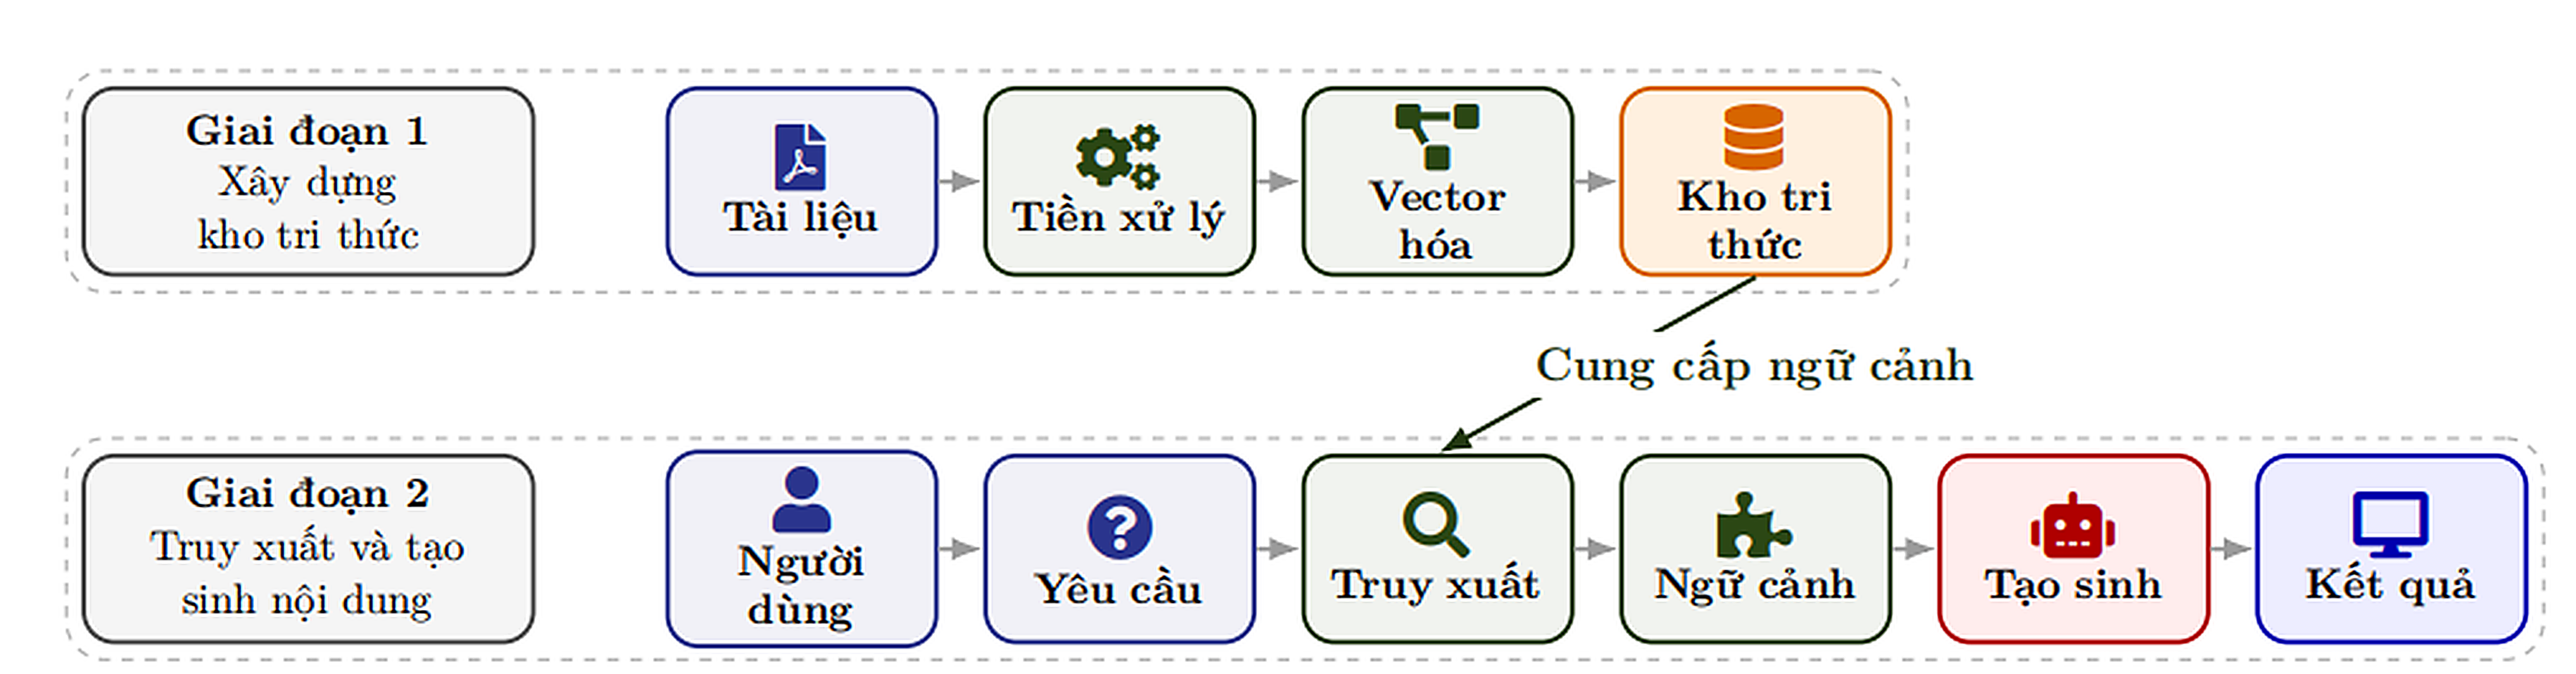
\includegraphics[width=0.9\linewidth]{Figures/pipeline.png}
\end{center}

\begin{figurecaptionmodern}
\capfig{Luồng hoạt động tổng thể của hệ thống RAG học tập cá nhân hóa.}
\end{figurecaptionmodern}

Sơ đồ trên cho thấy hệ thống gồm hai giai đoạn chính: giai đoạn 1 tập trung vào việc xử lý tài liệu đầu vào để xây dựng kho tri thức vector, và giai đoạn 2 khai thác kho tri thức đó để truy xuất ngữ cảnh, hỗ trợ LLM tạo sinh nội dung trả lời cho người dùng.

\subsection{Tiền xử lý và lưu trữ dữ liệu}

Mục tiêu của giai đoạn này là chuyển đổi các tài liệu học tập thành các đơn vị tri thức có cấu trúc và có khả năng truy xuất được. Hình 2 phác thảo chi tiết pipeline xử lý dữ liệu từ dạng thô cho đến khi được lưu trữ vào cơ sở dữ liệu vector.

\begin{center}
    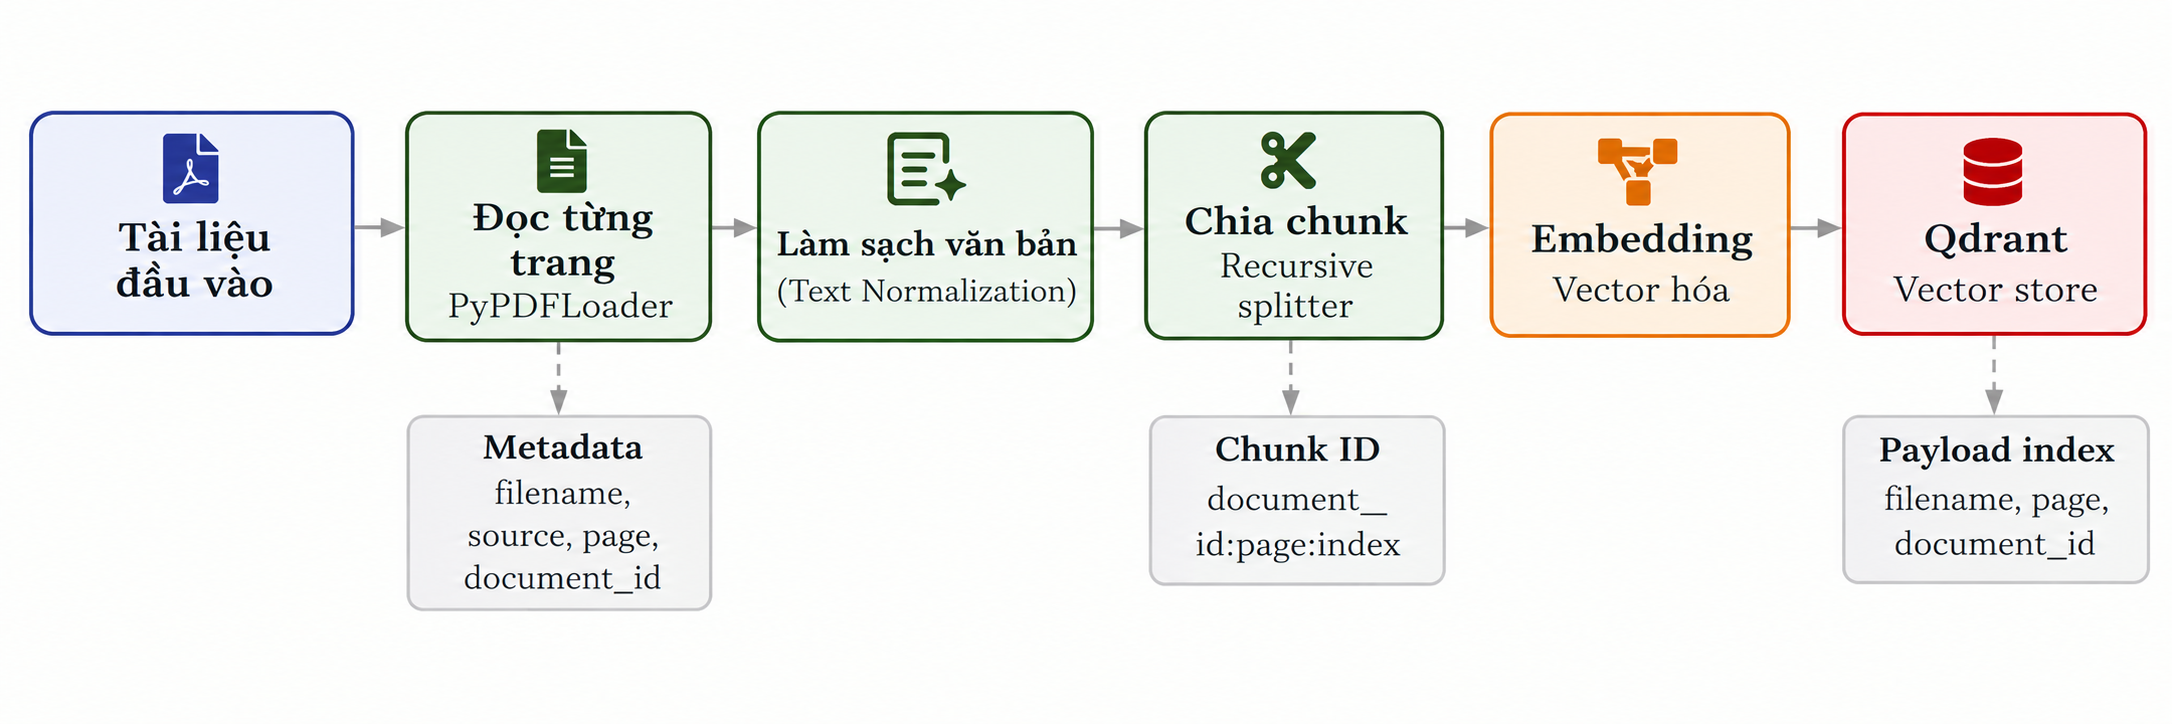
\includegraphics[width=0.9\linewidth]{Figures/data_pipeline.png}
\end{center}

\begin{figurecaptionmodern}
\capfig{Pipeline tiền xử lý tài liệu, chia chunk, vector hóa và lưu trữ vào Qdrant.}
\end{figurecaptionmodern}

Dựa vào sơ đồ trên, quá trình tiền xử lý được thực hiện qua các bước cụ thể như sau:

\begin{enumerate}
    \item \textbf{Nạp và trích xuất nội dung đa định dạng (Multi-format Ingestion):} Để mở rộng phạm vi ứng dụng trong môi trường học tập thực tế, hệ thống hỗ trợ 5 định dạng tài liệu học tập phổ biến bao gồm: Adobe PDF (\texttt{.pdf}), Microsoft Word (\texttt{.docx}), PowerPoint (\texttt{.pptx}), Markdown (\texttt{.md}) và Plain Text (\texttt{.txt}). Mỗi định dạng được xử lý qua bộ bóc tách chuyên biệt, tự động ánh xạ vị trí logic (số trang đối với PDF/Word, số slide đối với PowerPoint) và sinh mã băm SHA-1 \texttt{document\_id} duy nhất dựa trên tên và dung lượng tệp nhằm phục vụ cơ chế kiểm chứng trích dẫn nguồn sau này.
    
    \item \textbf{Chuẩn hóa và làm sạch văn bản:} Dữ liệu văn bản từ PDF thường chứa nhiều lỗi định dạng, ký tự đặc biệt hoặc nối chữ sai do quá trình parse. Hệ thống sử dụng module \texttt{src/utils/tf\_text\_utils.py}, tích hợp công cụ từ thư viện TensorFlow Text để chuẩn hóa Unicode, loại bỏ các ký tự rác và định dạng lại khoảng trắng. Bước này đóng vai trò quan trọng trong việc nâng cao chất lượng văn bản đầu vào cho mô hình Embedding.
    
    \item \textbf{Phân mảnh văn bản (Text Chunking):} Vì tài liệu học tập thường có dung lượng lớn, vượt qua giới hạn ngữ cảnh an toàn hoặc gây loãng sự chú ý của mô hình ngôn ngữ, văn bản cần được phân đoạn thành các đơn vị tri thức nhỏ (\textit{chunks}). Hệ thống hỗ trợ hai chiến lược phân đoạn có tính bổ trợ cao:
    \begin{itemize}
        \item \textit{Phân đoạn đệ quy theo ký tự (Recursive Character Chunking):} Cố định kích thước (mặc định 1000 ký tự, độ chồng lấp 150 ký tự). Thuật toán phân đoạn phân cấp theo thứ tự ưu tiên: dấu ngắt đoạn (\texttt{\textbackslash n\textbackslash n}), dấu ngắt câu (\texttt{.\ }), khoảng trắng từ (\texttt{\ }), giữ cho cấu trúc ngữ pháp tự nhiên không bị cắt gãy tùy tiện.
        \item \textit{Phân đoạn ngữ nghĩa động (Semantic Chunking based on Interquartile Distance):} Để khắc phục nhược điểm ngắt đoạn cơ học làm phân tán ngữ cảnh của phương pháp đệ quy, hệ thống tích hợp giải thuật phân đoạn ngữ nghĩa dựa trên phân phối khoảng cách cosine giữa các câu liên tiếp. Văn bản trước tiên được tách thành chuỗi các câu độc lập $(s_1, s_2, \dots, s_n)$. Mô hình embedding mã hóa từng câu thành các vector $\mathbf{v}_i \in \mathbb{R}^d$, từ đó tính toán khoảng cách cosine giữa hai câu kề cận:
        \begin{equation}
            d_i = 1 - \frac{\mathbf{v}_i \cdot \mathbf{v}_{i+1}}{\|\mathbf{v}_i\|_2 \|\mathbf{v}_{i+1}\|_2}
        \end{equation}
        Ngưỡng phân tách chủ đề động $T_{\text{split}}$ được xác định tự động dựa trên khoảng phân vị tứ phân vị (\textit{Interquartile Range} -- IQR):
        \begin{equation}
            T_{\text{split}} = Q_3 + 1.5 \times (Q_3 - Q_1) \quad \text{hoặc phân vị thích ứng } P_{\alpha} (\alpha = 0.85)
        \end{equation}
        Điểm cắt chỉ được tạo ra khi khoảng cách $d_i > T_{\text{split}}$, tương ứng với một bước chuyển dịch chủ đề rõ rệt. Nhờ đó, toàn bộ các định nghĩa, công thức và ví dụ liên quan được bảo toàn trọn vẹn trong cùng một khối tri thức thống nhất.
    \end{itemize}
    
    \item \textbf{Vector hóa và lưu trữ (Embedding \& Vector DB):} Mỗi văn bản sau khi được phân mảnh sẽ được đưa qua một mô hình nhúng (Embedding Model) từ HuggingFace để chuyển đổi thành một vector số thực biểu diễn ngữ nghĩa. Các vector này, cùng với metadata tương ứng, được đẩy vào cơ sở dữ liệu \textbf{Qdrant} (chạy ở chế độ local tại thư mục \texttt{qdrant\_storage/}). 
\end{enumerate}

Toàn bộ các thực thể dữ liệu truyền tải giữa các bước như thông tin metadata, dữ liệu chunk đều được chuẩn hóa nghiêm ngặt bằng \textit{Pydantic schemas} (trong file \texttt{src/core/schemas.py}). Hình 3 đây thể hiện mối quan hệ phân cấp và liên kết giữa các schema dữ liệu này.

\begin{center}
    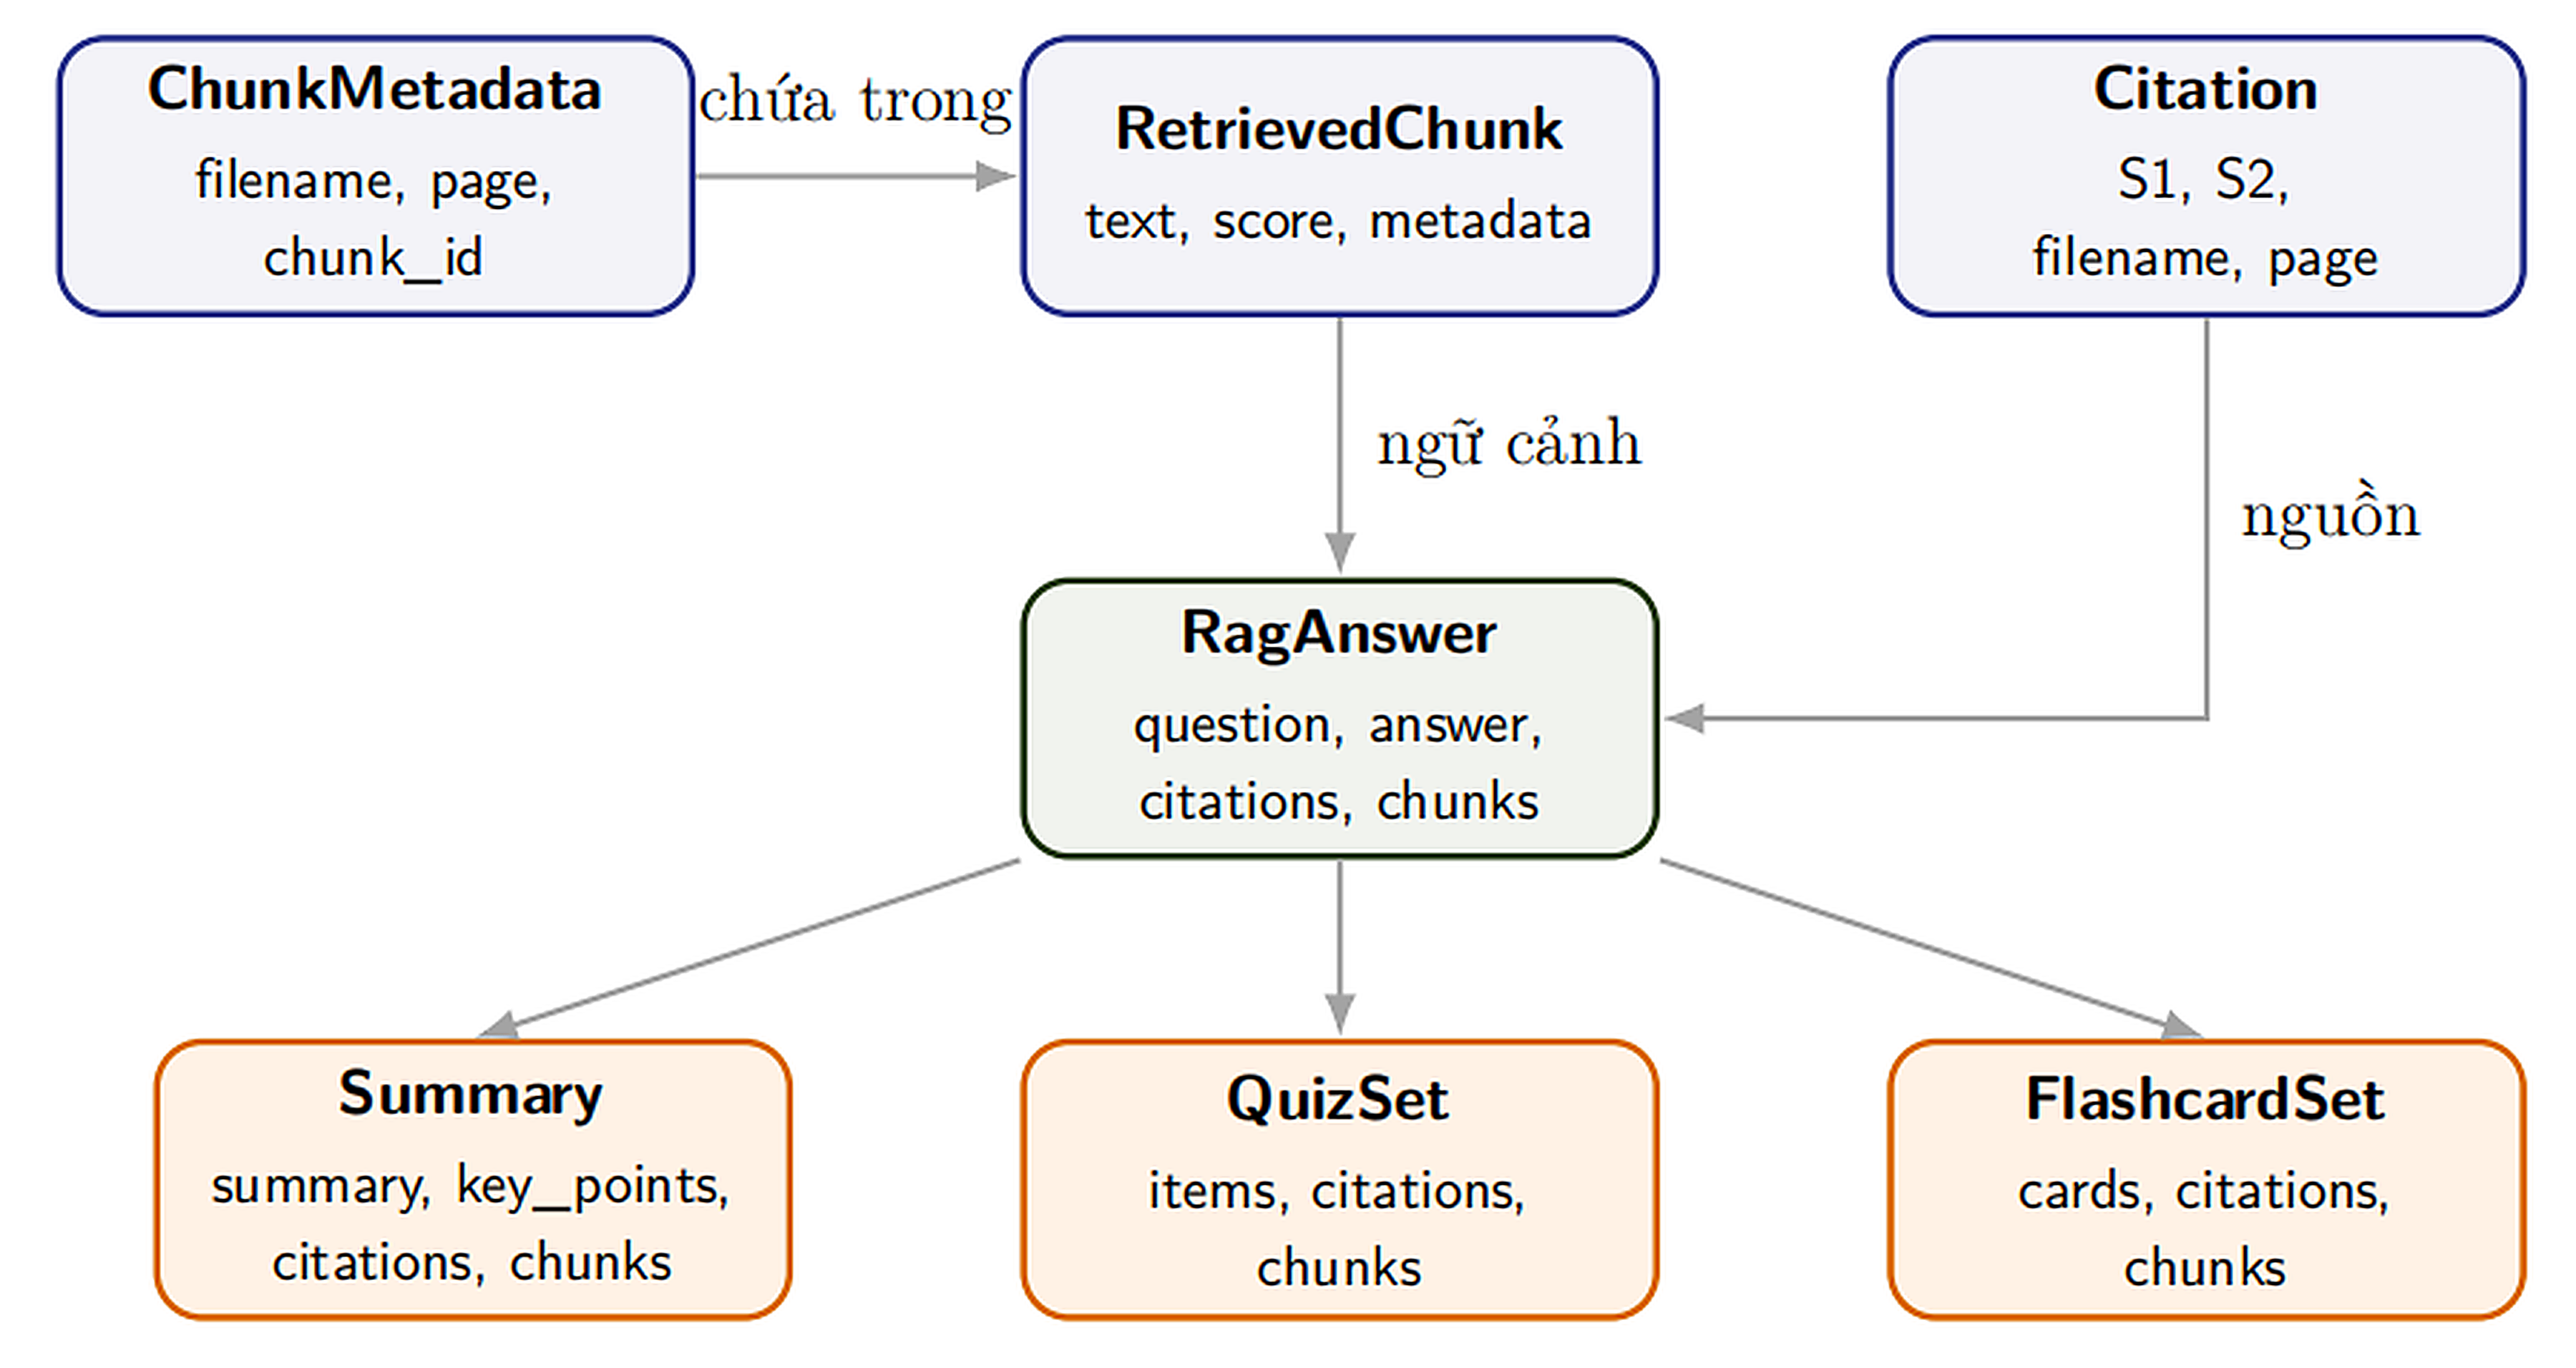
\includegraphics[width=0.85\linewidth]{Figures/schema.png}
\end{center}

\begin{figurecaptionmodern}
\capfig{Sơ đồ mối quan hệ giữa các Data Schemas chính trong hệ thống.}
\end{figurecaptionmodern}

Cấu trúc schema ở trên cho thấy \texttt{ChunkMetadata} luôn được nhúng gọn gàng vào bên trong \texttt{RetrievedChunk}, giúp hệ thống duy trì được nguồn gốc (citations) khi dữ liệu truyền tới bước cuối cùng như \texttt{RagAnswer} hay \texttt{Summary}. Thiết kế này đảm bảo tính nhất quán và dễ dàng bảo trì mở rộng cho các giai đoạn phát triển RAG tiếp theo.

\subsection{Pipeline truy xuất và tạo sinh RAG}

Pipeline truy xuất và tạo sinh (\textit{Retrieval-Augmented Generation} -- RAG) là module cốt lõi chịu trách nhiệm kết nối trực tiếp với cơ sở dữ liệu vector đã được lập chỉ mục ở giai đoạn trước (\ref{thesection}1), chuyển đổi các truy vấn tự nhiên của người học thành ngữ cảnh chính xác và sinh câu trả lời có khả năng kiểm chứng nguồn gốc. Để cân bằng tối ưu giữa độ bao phủ (\textit{Recall}) và độ chính xác của ngữ cảnh (\textit{Precision}), hệ thống được thiết kế theo kiến trúc truy xuất hai tầng kết hợp tái xếp hạng (\textit{Two-Stage Retrieval with Reranking}) \cite{xiao2023c, karpukhin2020dense}.

Hình 4 phác thảo toàn bộ quy trình vận hành tuần tự từ khi tiếp nhận câu hỏi của người học cho đến khi xuất ra đối tượng phản hồi có cấu trúc kèm trích dẫn nguồn.

\begin{center}
    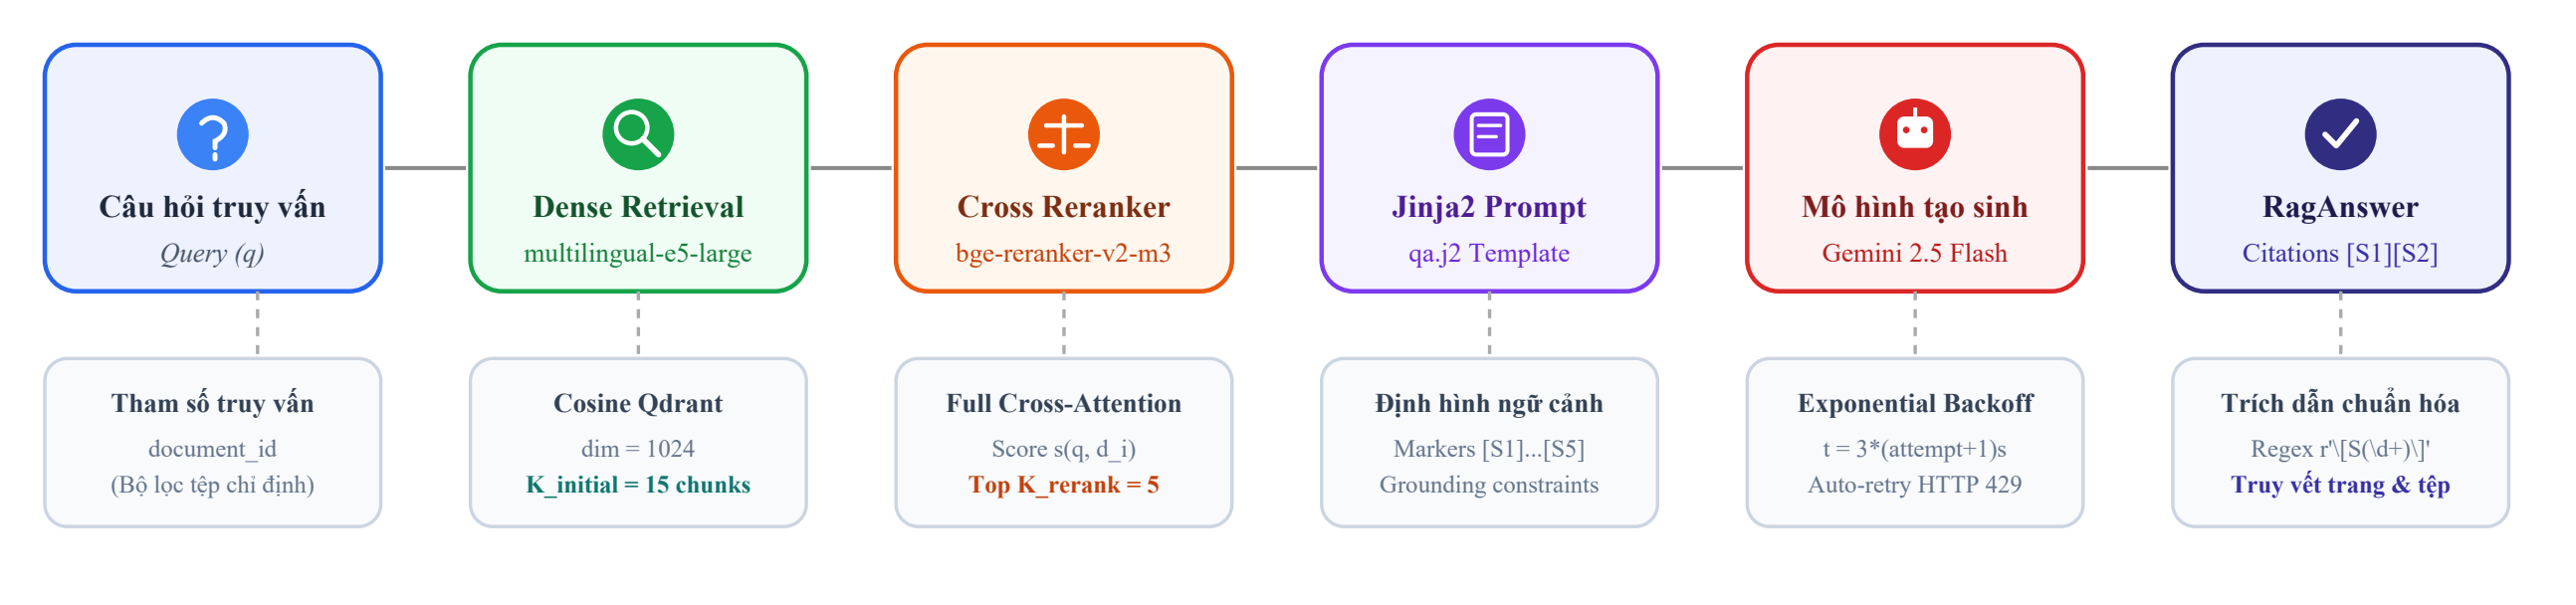
\includegraphics[width=0.92\linewidth]{Figures/rag_two_stage_pipeline.png}
\end{center}

\begin{figurecaptionmodern}
\capfig{Kiến trúc chi tiết của Pipeline RAG hai tầng: Semantic Retrieval kết hợp Cross-Encoder Reranking và cơ chế trích dẫn nguồn chuẩn xác.}
\end{figurecaptionmodern}

\subsubsection{Tầng 1: Truy xuất ngữ nghĩa sơ bộ (Dense Semantic Retrieval)}
Quy trình bắt đầu khi người dùng gửi một câu hỏi $q$. Nhằm thu hẹp khoảng cách từ vựng (\textit{lexical gap}), câu hỏi được chuyển đổi thành vector nhúng ngữ nghĩa $\mathbf{e}_q \in \mathbb{R}^{1024}$ bằng mô hình Bi-Encoder \texttt{intfloat/multilingual-e5-large} \cite{wang2024e5} chạy trên GPU (CUDA). Cơ sở dữ liệu Qdrant sau đó thực hiện tìm kiếm láng giềng gần nhất dựa trên độ đo tương đồng Cosine:
\begin{equation}
    \text{sim}(q, d_i) = \frac{\mathbf{e}_q \cdot \mathbf{e}_{d_i}}{\|\mathbf{e}_q\|_2 \|\mathbf{e}_{d_i}\|_2}
\end{equation}
Trong đó $\mathbf{e}_{d_i}$ là vector embedding của đoạn văn bản thứ $i$ đã được tiền xử lý và lưu trữ trong bộ sưu tập \texttt{documents}. 

Điểm nổi bật trong thiết kế của hệ thống là khả năng kiểm soát phạm vi tìm kiếm thông qua trường \texttt{document\_id}. Nhờ vào chỉ mục \textit{payload index} đã được khởi tạo ở giai đoạn tiền xử lý, hệ thống hỗ trợ hai chế độ truy xuất linh hoạt:
\begin{itemize}
    \item \textbf{Truy vấn cục bộ (Document-scoped):} Giới hạn không gian tìm kiếm trong duy nhất một tài liệu cụ thể bằng bộ lọc chính xác \texttt{FieldCondition(key="document\_id", match=MatchValue(value=doc\_id))}. Chế độ này thích hợp khi người học đang tập trung nghiên cứu một giáo trình hoặc chương bài học nhất định.
    \item \textbf{Truy vấn toàn cục (Global library):} Thực hiện tìm kiếm không lọc trên toàn bộ các tài liệu hiện có trong hệ thống, phục vụ việc đối chiếu và tổng hợp kiến thức liên môn.
\end{itemize}

Nhằm hạn chế rủi ro bỏ sót thông tin liên quan ở tầng lọc thô (False Negatives), hệ thống thiết lập ngưỡng thu hồi ban đầu rộng với $K_{\text{initial}} = 15$ chunks thay vì lấy ngay số lượng nhỏ.

\subsubsection{Tầng 2: Tái xếp hạng chuyên sâu bằng Cross-Encoder (Cross-Encoder Reranking)}
Mặc dù mô hình Bi-Encoder có tốc độ tìm kiếm cực nhanh nhờ việc tính toán trước vector tài liệu, việc mã hóa tách biệt câu hỏi và văn bản ngăn cản mô hình nắm bắt được sự tương tác qua lại phức tạp giữa các từ ngữ. Do đó, tầng thứ hai áp dụng mô hình Cross-Encoder \texttt{BAAI/bge-reranker-v2-m3} \cite{chen2024bge_m3}.

Tại tầng này, từng cặp gồm câu hỏi và nội dung chunk $(q, d_i)$ được ghép nối thành một chuỗi văn bản duy nhất và nạp đồng thời vào mạng Transformer. Cơ chế \textit{Full Self-Attention} cho phép mỗi token trong câu hỏi tương tác trực tiếp với từng token trong đoạn văn bản:
\begin{equation}
    s_i = \text{CrossEncoder}(q, d_i) = \text{Softmax}\left(\mathbf{W} \cdot \mathbf{h}_{[CLS]} + b\right)
\end{equation}
Trong đó $\mathbf{h}_{[CLS]}$ là vector biểu diễn ẩn của token đặc biệt $[CLS]$ tại tầng cuối cùng. Điểm số $s_i$ thể hiện mức độ liên quan ngữ nghĩa thực tế một cách chính xác vượt trội so với khoảng cách cosine thô. Toàn bộ 15 đoạn văn bản ứng viên được sắp xếp lại theo chiều giảm dần của $s_i$, và hệ thống chỉ giữ lại top $K_{\text{rerank}} = 5$ đoạn văn bản có chất lượng cao nhất để đưa vào ngữ cảnh sinh câu trả lời.

Bảng 1 tóm tắt và so sánh các thông số kỹ thuật cốt lõi giữa hai tầng truy xuất trong hệ thống.

\begin{table}[H]
\centering
\small
\begin{tabularx}{\linewidth}{@{}l p{4.2cm} p{2.8cm} c p{4.5cm}@{}}
\toprule
\textbf{Tầng truy xuất} & \textbf{Mô hình sử dụng} & \textbf{Đầu ra / Chiều} & \textbf{Số lượng ($K$)} & \textbf{Mục tiêu tối ưu hóa} \\
\midrule
\textbf{Tầng 1 (Bi-Encoder)} & \texttt{intfloat/multilingual-e5-large} & $\mathbb{R}^{1024}$ (Dense vector) & $K_{\text{initial}} = 15$ & Tối đa hóa độ bao phủ (\textit{Recall}), tìm kiếm thời gian thực trên Qdrant. \\
\addlinespace[4pt]
\textbf{Tầng 2 (Cross-Encoder)} & \texttt{BAAI/bge-reranker-v2-m3} & $s_i \in [0, 1]$ (Relevance score) & $K_{\text{rerank}} = 5$ & Tối đa hóa độ chính xác (\textit{Precision}), loại bỏ nhiễu ngữ cảnh. \\
\bottomrule
\end{tabularx}
\caption{So sánh đặc tính kỹ thuật giữa hai tầng trong kiến trúc Two-Stage Retrieval.}
\end{table}

\subsubsection{Cơ chế Truy xuất Lai và Hợp nhất Điểm số (Hybrid Search via RRF)}
Trong môi trường học thuật chuyên sâu, người học thường truy vấn các thuật ngữ viết tắt (ví dụ: \texttt{DPO}, \texttt{RLHF}, \texttt{LoRA}, \texttt{PEFT}) hoặc các công thức ký hiệu kỹ thuật. Mô hình Bi-Encoder Dense Retrieval tuy rất mạnh về khả năng hiểu ngữ nghĩa bao quát, nhưng lại bộc lộ ``điểm mù từ vựng'' (\textit{Lexical Blind Spot}) khi đối mặt với các chuỗi ký tự viết tắt hiếm hoặc có tần suất xuất hiện thấp trong không gian vector.

Nhằm triệt tiêu điểm mù này, hệ thống tích hợp công nghệ \textbf{Truy xuất Lai (Hybrid Search)}, phối hợp song song hai giải thuật tìm kiếm độc lập:
\begin{enumerate}
    \item \textbf{Truy xuất từ khóa rời rạc (Sparse Retrieval):} Sử dụng thuật toán BM25 Okapi \cite{robertson2009probabilistic} để tính điểm tương đồng từ vựng dựa trên tần số xuất hiện của từ ($f(t, d)$) và nghịch đảo tần số tài liệu ($\text{IDF}$):
    \begin{equation}
        \text{Score}_{\text{BM25}}(q, d) = \sum_{t \in q} \text{IDF}(t) \cdot \frac{f(t, d) \cdot (k_1 + 1)}{f(t, d) + k_1 \cdot \left(1 - b + b \cdot \frac{|d|}{\text{avgdl}}\right)}
    \end{equation}
    với $k_1 = 1.5$, $b = 0.75$. BM25 đảm bảo các chunk chứa chính xác từ khóa viết tắt luôn đạt điểm số cao nhất.
    \item \textbf{Truy xuất ngữ nghĩa mật (Dense Retrieval):} Sử dụng mô hình Multilingual-E5-large trên không gian vector Cosine nhằm bao quát các câu hỏi diễn đạt tự nhiên, đồng nghĩa hoặc suy luận ngữ cảnh.
\end{enumerate}

Để hợp nhất kết quả từ hai không gian điểm số có phân phối và độ lớn hoàn toàn khác nhau, hệ thống áp dụng giải thuật \textbf{Reciprocal Rank Fusion (RRF)} \cite{cormack2009reciprocal}:
\begin{equation}
    \text{Score}_{\text{RRF}}(d) = \sum_{m \in \{\text{Dense}, \text{BM25}\}} \frac{1}{k + r_m(d)}
\end{equation}
trong đó $k = 60$ là hằng số làm mượt xếp hạng, $r_m(d) \in [1, K]$ là thứ hạng của tài liệu $d$ trong danh sách trả về từ phương pháp $m$. Danh sách top ứng viên sau khi dung hợp RRF sẽ được chuyển thẳng tới Tầng 2 (BGE Cross-Encoder Reranker) để tinh chế lại một lần nữa. Sự phối hợp đa tầng này hình thành nên kiến trúc hoàn chỉnh có tên gọi \textbf{Golden Fusion} --- cấu hình được thực nghiệm chứng minh đạt hiệu năng vượt trội nhất ở Mục IV.

\subsubsection{Cấu trúc ngữ cảnh, Prompt Engineering và Ràng buộc sinh}
Top 5 chunks sau khi được chọn lọc sẽ được chuyển qua bộ render mẫu Jinja2 (\texttt{src/prompts/qa.j2}). Mỗi đoạn ngữ cảnh được định danh một nhãn nguồn chuẩn hóa theo định dạng $[S_1], [S_2], \dots, [S_5]$ kèm số trang và tên file tài liệu gốc:
\begin{center}
\texttt{[S1] (Tài liệu: GiaoTrinhAI.pdf, Trang: 42): <Nội dung đoạn trích 1>}
\end{center}

Mẫu prompt được thiết kế với các ràng buộc căn cứ tri thức (\textit{grounding constraints}) nghiêm ngặt:
\begin{enumerate}[(1)]
    \item \textbf{Căn cứ tri thức (Strict Grounding):} Mô hình sinh bắt buộc chỉ dựa vào các sự kiện có căn cứ trực tiếp trong ngữ cảnh được cung cấp; tuyệt đối không sử dụng các tri thức ngoại lai ngoài tài liệu.
    \item \textbf{Gắn nhãn trích dẫn tường minh (In-text Citations):} Yêu cầu LLM gắn trực tiếp các thẻ định danh $[S_i]$ ngay sau mỗi mệnh đề hoặc kết luận thông tin trong câu trả lời. Điều này cho phép người học đối chiếu và xác thực nguồn gốc thông tin trong tích tắc.
    \item \textbf{Kháng ảo giác (Anti-hallucination):} Nếu thông tin trong ngữ cảnh không đủ để khẳng định câu trả lời, mô hình phải từ chối lịch sự bằng thông điệp chuẩn hóa, ngăn chặn hoàn toàn hiện tượng suy đoán vô căn cứ \cite{ji2023survey}.
\end{enumerate}

\subsubsection{Lớp trừu tượng hóa LLM và Cơ chế phục hồi lỗi}
Nhằm đảm bảo tính độc lập và khả năng hoán đổi linh hoạt giữa các nhà cung cấp mô hình ngôn ngữ lớn, hệ thống triển khai lớp giao diện trừu tượng \texttt{LLMBackend} (\texttt{src/llm.py}). Hệ thống hỗ trợ 3 backend:
\begin{itemize}
    \item \textbf{GeminiBackend (Chính thức):} Tích hợp mô hình \texttt{gemini-2.5-flash} thông qua Google Generative AI SDK. Mô hình này sở hữu tốc độ sinh vượt trội, khả năng tuân thủ định dạng thẻ trích dẫn inline cực kỳ chuẩn xác. Đặc biệt, backend này được cài đặt cơ chế xử lý lỗi tự động với thuật toán \textit{Exponential Backoff}: khi gặp giới hạn tần suất (HTTP 429 / \texttt{RESOURCE\_EXHAUSTED}), hệ thống tự động tạm dừng $t_{\text{wait}} = 3 \times (\text{attempt} + 1)$ giây và thử lại tối đa 4 lần trước khi báo lỗi.
    \item \textbf{HFLocalBackend:} Cho phép tải trực tiếp các mô hình ngôn ngữ mã nguồn mở (như Qwen2.5, LLaMA-3) chạy trên GPU cục bộ qua thư viện HuggingFace Transformers.
    \item \textbf{vLLMBackend:} Kết nối máy chủ phục vụ mô hình ngôn ngữ phân tán hiệu năng cao thông qua chuẩn REST API tương thích OpenAI.
\end{itemize}

Sau khi LLM hoàn tất quá trình tạo sinh văn bản, module bóc tách nguồn sử dụng biểu thức chính quy \texttt{r'\[S(\d+)\]'} để quét toàn bộ các thẻ $[S_i]$ xuất hiện trong nội dung trả lời theo chuẩn ALCE \cite{gao2023alce}. Hệ thống tự động ánh xạ ngược lại các chunk tương ứng trong danh sách 5 chunks ban đầu, tạo ra danh sách đối tượng \texttt{Citation} (chứa marker, nội dung trích dẫn và metadata số trang), sau đó đóng gói toàn bộ vào schema \texttt{RagAnswer}.

\subsection{Chức năng học tập thông minh}

Không dừng lại ở việc hỏi đáp tra cứu bị động, hệ thống tận dụng nguồn tri thức đã phân mảnh để xây dựng một bộ công cụ học tập chủ động và cá nhân hóa, bao gồm: Tóm tắt tài liệu thích ứng, Sinh bài thi trắc nghiệm và Tạo bộ thẻ ghi nhớ Flashcards.

\subsubsection{Tóm tắt tài liệu thích ứng (Adaptive Hierarchical Summarization)}
Các tài liệu học tập như giáo trình, sách chuyên khảo thường có độ dài hàng chục tới hàng trăm trang, vượt quá giới hạn ngữ cảnh an toàn của LLM hoặc gây ra hiện tượng suy giảm chú ý ở phần giữa văn bản (\textit{Lost in the Middle}) \cite{liu2023lost}. Để giải quyết triệt để rào cản này, hệ thống áp dụng cơ chế tóm tắt thích ứng dựa trên nguyên lý xử lý đệ quy cho văn bản dài \cite{wu2021recursive_summarize} kết hợp số lượng chunk $N$ thực tế của tài liệu trích xuất qua Qdrant Scroll API (\texttt{fetch\_all\_chunks}):

Hình 5 minh họa trực quan hai luồng xử lý phân nhánh của cơ chế tóm tắt thích ứng.

\begin{center}
    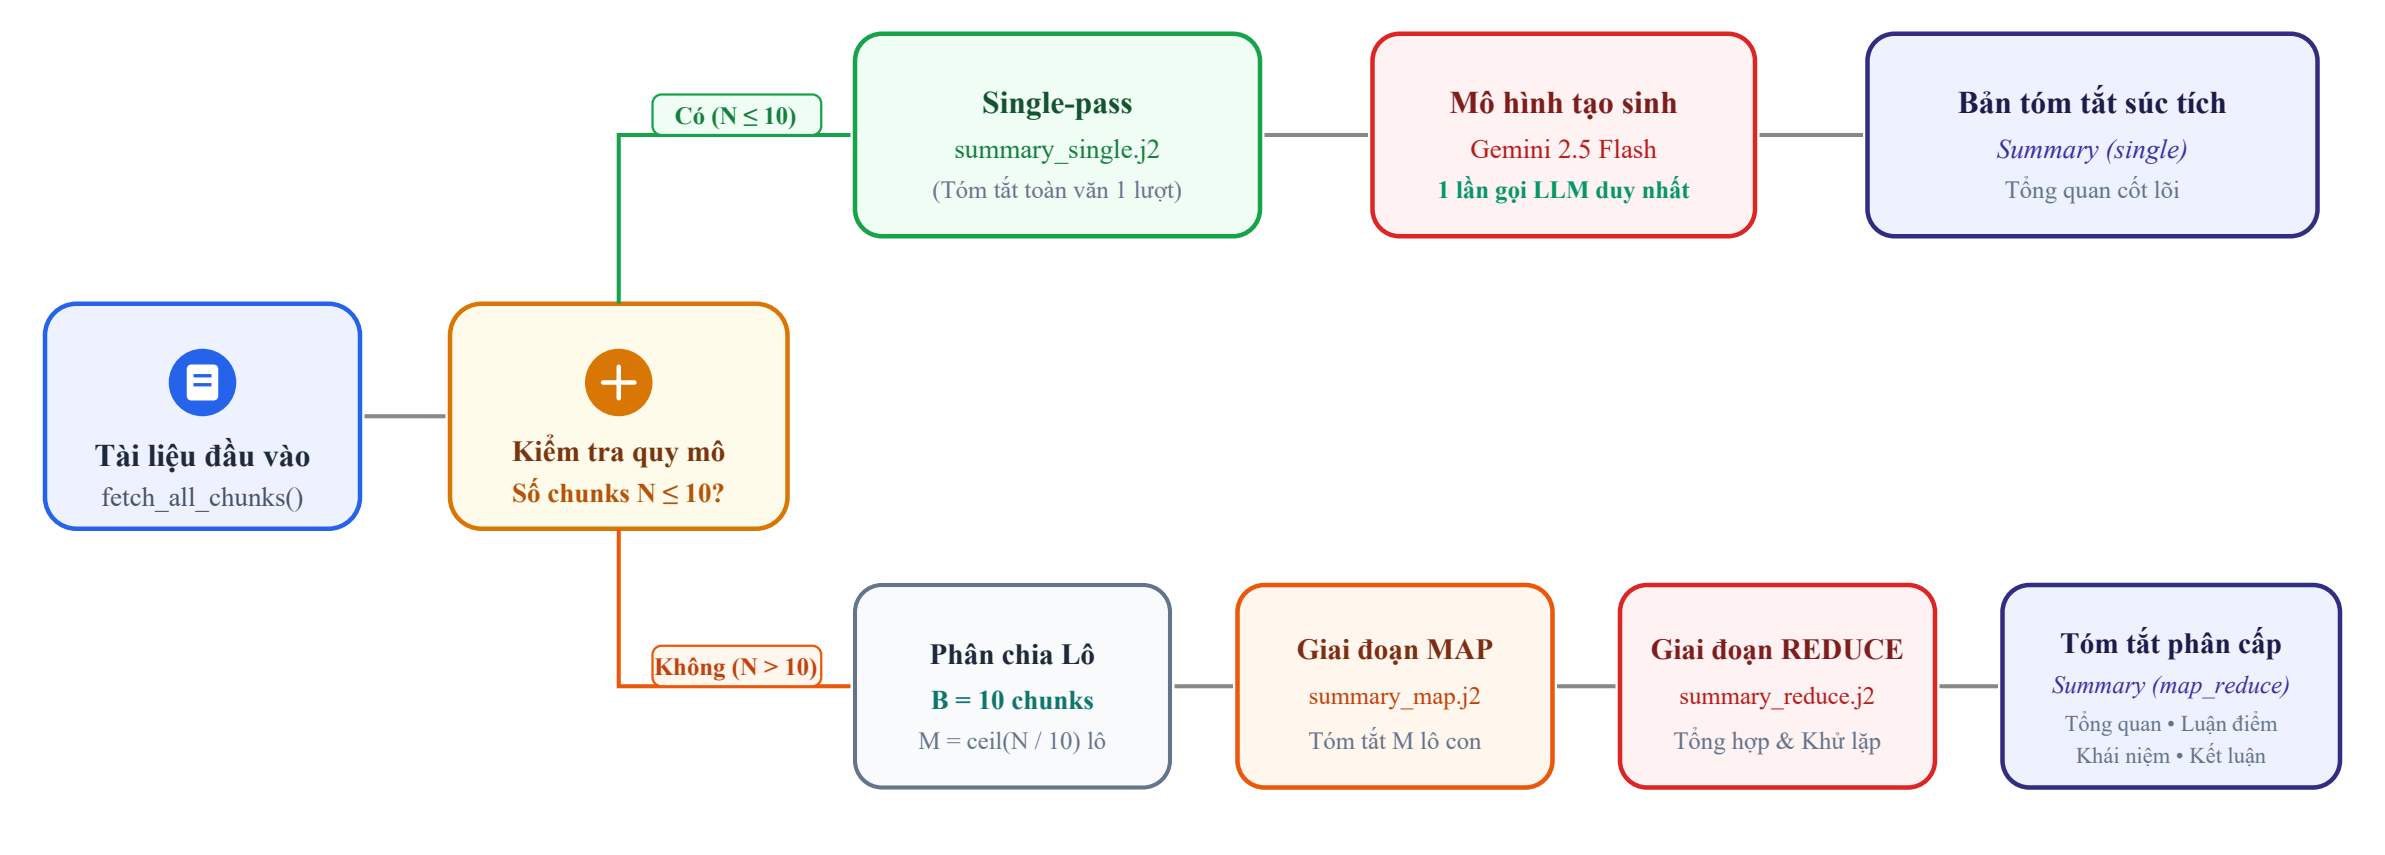
\includegraphics[width=0.92\linewidth]{Figures/map_reduce_pipeline.png}
\end{center}

\begin{figurecaptionmodern}
\capfig{Quy trình tóm tắt thích ứng: Tự động phân luồng giữa Single-pass (tài liệu ngắn) và Hierarchical Map-Reduce (tài liệu dài).}
\end{figurecaptionmodern}

\begin{itemize}
    \item \textbf{Nhánh 1: Tóm tắt một lượt (Single-pass, $N \le 10$ chunks):} Áp dụng cho các tài liệu ngắn dưới 10 trang. Toàn bộ nội dung chunks được ghép nối theo thứ tự xuất hiện và gửi trực tiếp tới mẫu template \texttt{summary\_single.j2}. LLM sinh bản tóm tắt nhanh chóng chỉ trong một lần gọi API duy nhất.
    \item \textbf{Nhánh 2: Tóm tắt phân cấp Map-Reduce ($N > 10$ chunks):} Áp dụng cho các tài liệu quy mô lớn, được thực hiện theo 2 giai đoạn kế tiếp:
    \begin{enumerate}
        \item \textit{Giai đoạn Map:} Toàn bộ $N$ chunks được phân chia thành $M = \lceil N / B \rceil$ lô nhỏ (batch) với kích thước cố định $B = 10$ chunks. Từng lô được đưa qua template \texttt{summary\_map.j2} để LLM tóm tắt độc lập, cô đọng nội dung cục bộ của từng phần thành các bản tóm tắt trung gian (\textit{intermediate summaries}).
        \item \textit{Giai đoạn Reduce:} Hệ thống tập hợp toàn bộ $M$ bản tóm tắt trung gian và chuyển vào template \texttt{summary\_reduce.j2}. Tại đây, LLM thực hiện tổng hợp mức cao: loại bỏ các luận điểm trùng lặp, xâu chuỗi các mạch logic xuyên suốt tài liệu và cấu trúc thành bản tóm tắt toàn diện gồm: Tổng quan khái quát, Các luận điểm cốt lõi, Danh mục khái niệm quan trọng và Kết luận rút ra.
    \end{enumerate}
\end{itemize}

\subsubsection{Tạo bộ câu hỏi trắc nghiệm tương tác và Thẻ ghi nhớ ôn tập}
Để kích thích việc ôn tập chủ động (\textit{Active Recall}) và ghi nhớ ngắt quãng (\textit{Spaced Repetition}) theo các nguyên lý tâm lý học giáo dục \cite{kasneci2023education}, hệ thống cung cấp hai module tự động sinh học liệu từ tài liệu gốc.

Hình 6 thể hiện luồng xử lý dữ liệu và kiến trúc phòng vệ hai lớp khi sinh bài kiểm tra trắc nghiệm MCQ và bộ thẻ Flashcards.

\begin{center}
    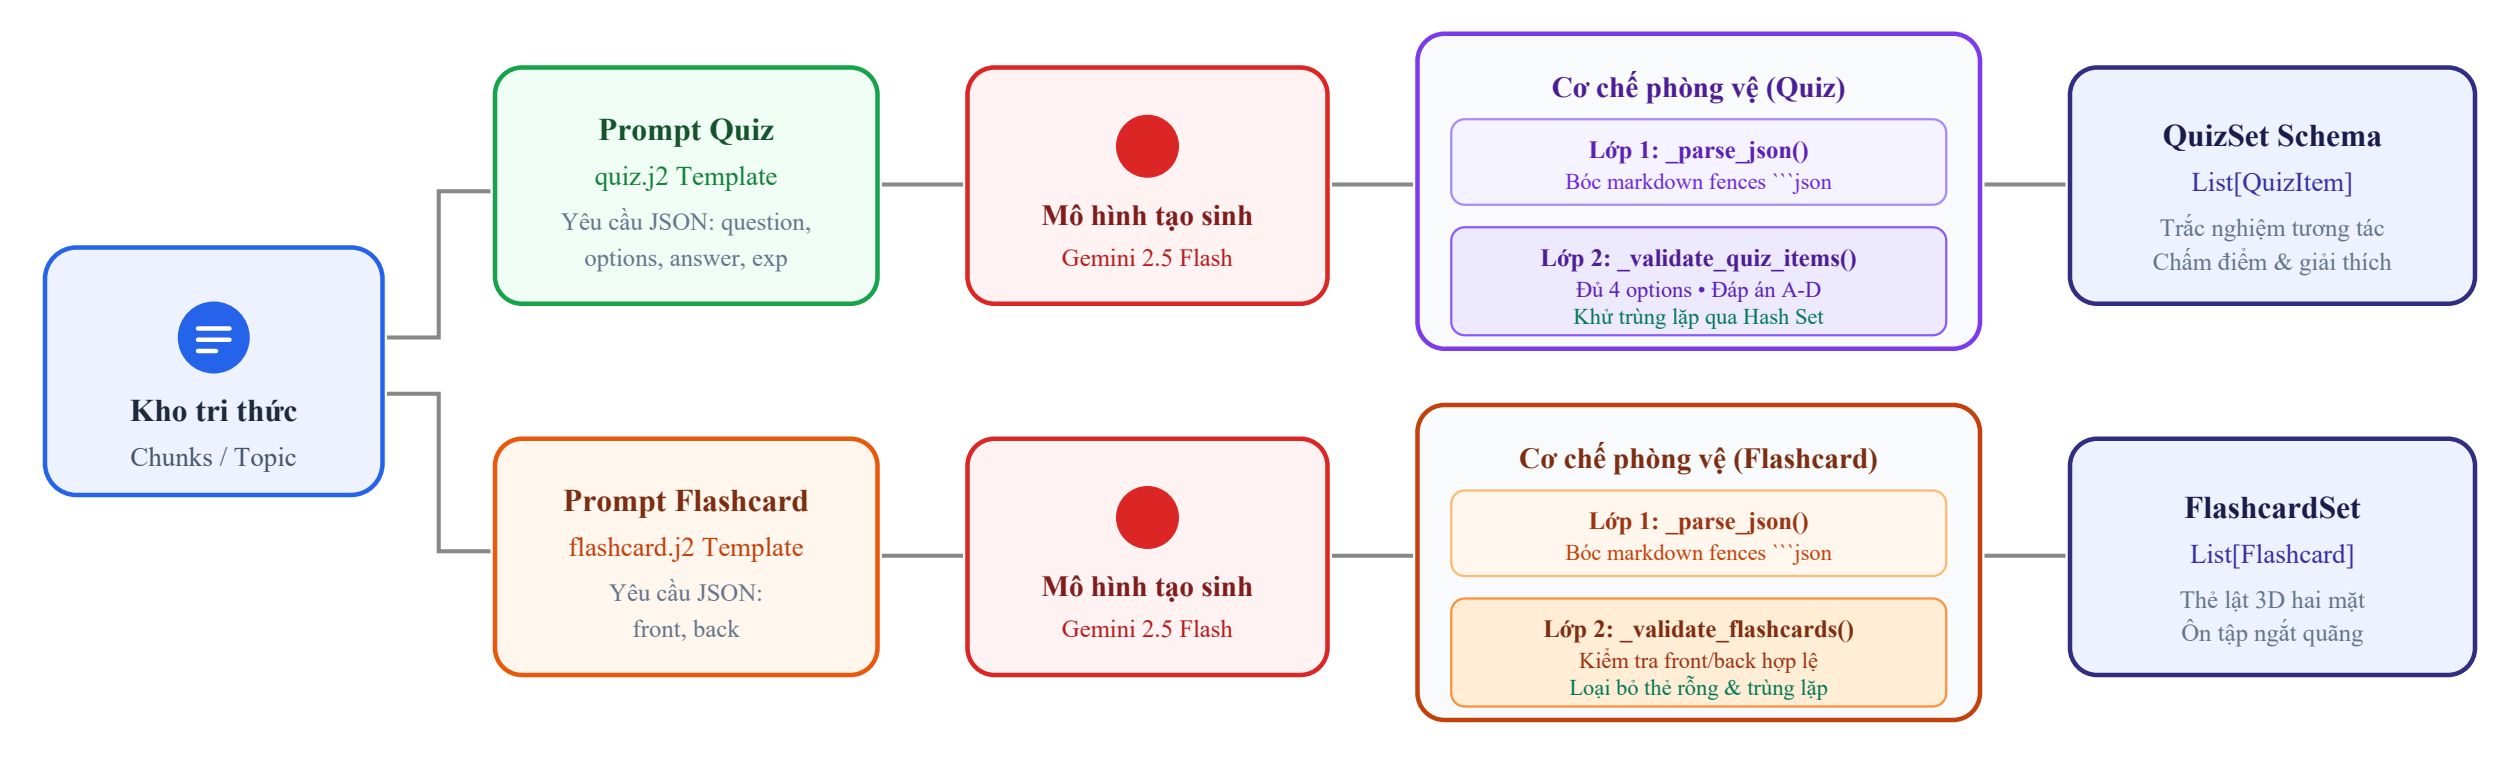
\includegraphics[width=0.92\linewidth]{Figures/learning_features_flow.png}
\end{center}

\begin{figurecaptionmodern}
\capfig{Luồng tạo câu hỏi trắc nghiệm MCQ và Flashcards tích hợp cơ chế xác thực và chuẩn hóa dữ liệu phòng vệ hai lớp.}
\end{figurecaptionmodern}

\paragraph{A. Sinh bộ câu hỏi trắc nghiệm (MCQ Quiz Generation):}
Module \texttt{generate\_quiz()} cho phép tạo ra các câu hỏi trắc nghiệm khách quan 4 phương án ($A, B, C, D$) dựa trên toàn bộ tài liệu hoặc theo một chủ đề chỉ định (\textit{topic}). Mẫu \texttt{quiz.j2} chỉ dẫn LLM đóng vai trò chuyên gia sư phạm, thiết kế các câu hỏi có độ phân hóa từ mức nhận biết đến vận dụng kiến thức, kèm theo phương án đúng và lời giải thích cặn kẽ.

\paragraph{B. Sinh thẻ ghi nhớ (Flashcards Generation):}
Module \texttt{generate\_flashcards()} trích xuất các cặp thuật ngữ cốt lõi và định nghĩa trọng tâm thông qua mẫu \texttt{flashcard.j2}. Mỗi thẻ được cấu trúc hóa theo schema \texttt{Flashcard} gồm Mặt trước (\texttt{front}: thuật ngữ, công thức hoặc khái niệm) và Mặt sau (\texttt{back}: câu trả lời cô đọng, chính xác).

\paragraph{C. Cơ chế xác thực phòng vệ hai lớp (Two-Stage Defensive Validation):}
Mô hình sinh LLM thường có đặc tính ngẫu nhiên và dễ xuất ra dữ liệu có định dạng lỗi (như bao bọc JSON trong các thẻ markdown code fences \texttt{```json ... ```} hoặc kèm lời thoại phụ). Để ngăn chặn lỗi hệ thống, toàn bộ phản hồi dạng JSON đều phải vượt qua hai tầng kiểm duyệt nghiêm ngặt:
\begin{enumerate}
    \item \textbf{Lớp 1 -- Bóc tách và làm sạch JSON (\texttt{\_parse\_json}):} Sử dụng biểu thức chính quy để bóc tách chính xác phần thân JSON nằm giữa các khối markdown fence hoặc tìm kiếm vùng chứa dấu ngoặc vuông \texttt{[...]} / ngoặc nhọn \texttt{\{...\}}, loại bỏ hoàn toàn các ký tự dư thừa bên ngoài.
    \item \textbf{Lớp 2 -- Thẩm định tính toàn vẹn và chuẩn hóa (\texttt{\_validate\_items}):} Đối với Quiz, hệ thống xác minh sự tồn tại của đủ 4 trường dữ liệu bắt buộc (\texttt{question}, \texttt{options}, \texttt{answer}, \texttt{explanation}); kiểm tra danh sách phương án có chính xác 4 lựa chọn; chuẩn hóa ký tự đáp án về chữ cái hoa duy nhất ($A, B, C, D$); và sử dụng cấu trúc \textit{Hash Set} để loại trừ các câu hỏi bị trùng lặp nội dung. Các mục không thỏa mãn điều kiện sẽ bị loại bỏ an toàn trước khi đóng gói thành \texttt{QuizSet} hoặc \texttt{FlashcardSet}.
\end{enumerate}

\subsection{Kiến trúc giao diện người dùng đa kênh}

Để đưa toàn bộ năng lực của hệ thống AI vào ứng dụng thực tế phục vụ đa dạng nhóm người dùng (sinh viên, giảng viên, và nhà phát triển tích hợp), đồ án triển khai kiến trúc 3 kênh giao diện độc lập kết nối tới tầng AI Core Pipelines.

Hình 7 mô tả sơ đồ kiến trúc phân tầng (\textit{Tiered Architecture}) của hệ thống giao diện.

\begin{center}
    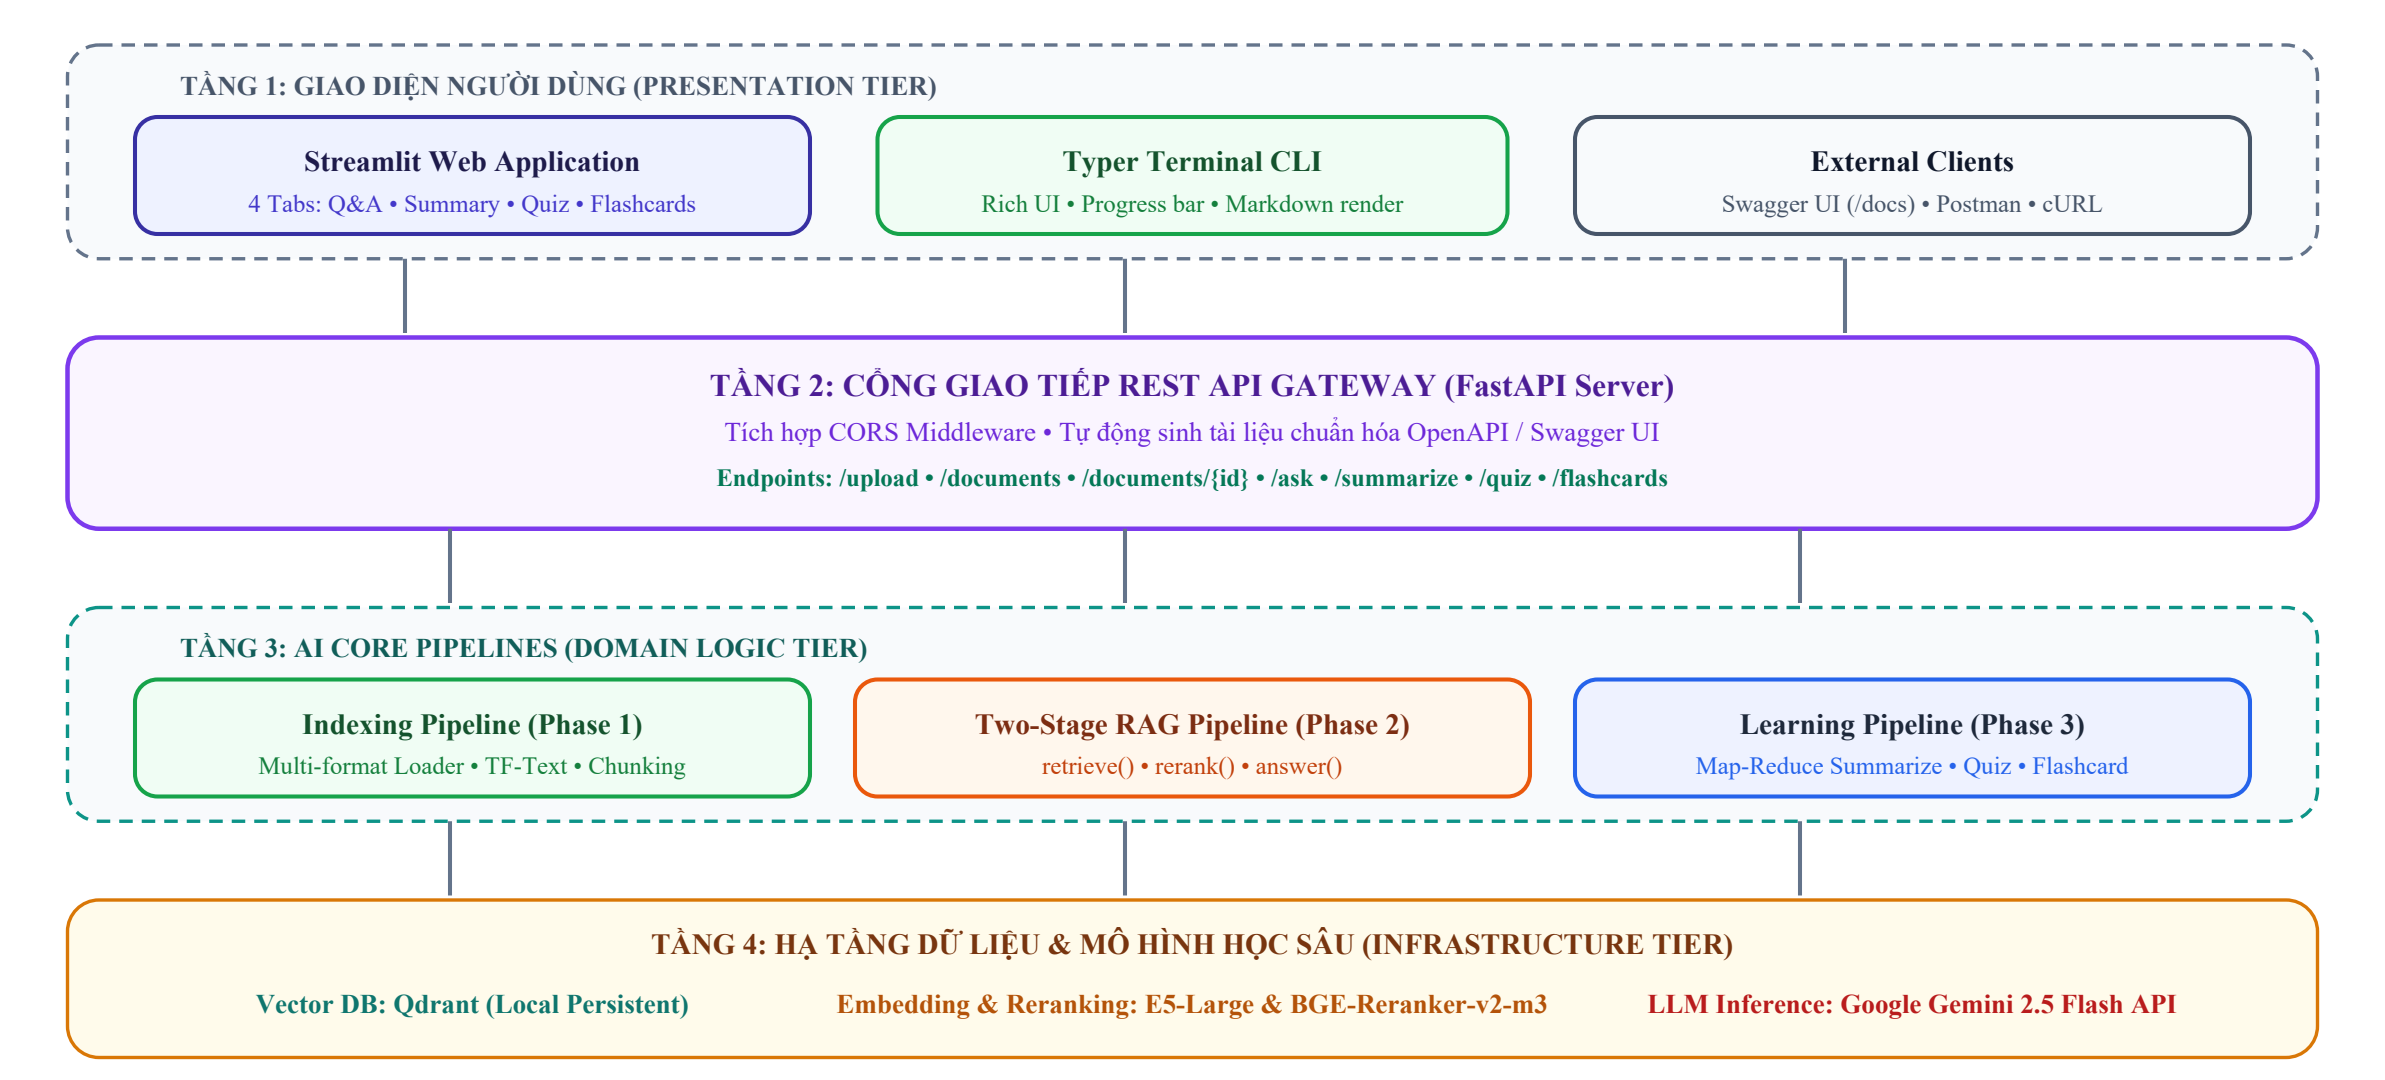
\includegraphics[width=0.92\linewidth]{Figures/interfaces_architecture.png}
\end{center}

\begin{figurecaptionmodern}
\capfig{Sơ đồ kiến trúc phân tầng của hệ thống giao diện: Kết nối từ Web UI, CLI và External Clients thông qua API Gateway tới AI Core Pipelines.}
\end{figurecaptionmodern}

\subsubsection{Kênh 1: FastAPI REST API Gateway (\texttt{src/interfaces/api.py})}
Máy chủ FastAPI đóng vai trò là cổng giao tiếp chuẩn hóa (\textit{API Gateway}) cho toàn bộ hệ sinh thái, cho phép các ứng dụng bên ngoài dễ dàng tích hợp qua chuẩn giao thức HTTP/JSON. Máy chủ cấu hình \textit{CORS Middleware} cho phép truy cập chéo tên miền và tự động phát sinh tài liệu tương tác Swagger UI tại đường dẫn \texttt{/docs}.

Bảng 2 liệt kê chi tiết các REST API endpoints được triển khai trong hệ thống.

\begin{table}[H]
\centering
\small
\begin{tabularx}{\linewidth}{@{}l l p{3.2cm} p{2.6cm} X@{}}
\toprule
\textbf{Endpoint} & \textbf{Method} & \textbf{Request Body} & \textbf{Response Model} & \textbf{Chức năng nghiệp vụ} \\
\midrule
\texttt{/upload} & \texttt{POST} & Multipart form (\texttt{file}) & \texttt{UploadResponse} & Tiếp nhận PDF/Word/PPTX, xử lý chunking, embed và lưu vào Qdrant. \\
\addlinespace[3pt]
\texttt{/documents} & \texttt{GET} & Không & \texttt{List[DocumentInfo]} & Liệt kê danh mục tài liệu đã nạp, số chunk và dung lượng. \\
\addlinespace[3pt]
\texttt{/documents/\{id\}} & \texttt{DELETE} & URL parameter (\texttt{doc\_id}) & \texttt{DeleteResponse} & Xóa vĩnh viễn tài liệu và các vector tương ứng khỏi Qdrant. \\
\addlinespace[3pt]
\texttt{/ask} & \texttt{POST} & \texttt{AskRequest} & \texttt{RagAnswer} & Truy vấn RAG hai tầng, trả về câu trả lời kèm danh sách trích dẫn nguồn. \\
\addlinespace[3pt]
\texttt{/summarize} & \texttt{POST} & \texttt{SummarizeRequest} & \texttt{Summary} & Kích hoạt tóm tắt thích ứng (Single-pass hoặc Map-Reduce). \\
\addlinespace[3pt]
\texttt{/quiz} & \texttt{POST} & \texttt{QuizRequest} & \texttt{QuizSet} & Sinh bộ đề thi trắc nghiệm khách quan 4 lựa chọn theo chủ đề. \\
\addlinespace[3pt]
\texttt{/flashcards} & \texttt{POST} & \texttt{FlashcardsRequest} & \texttt{FlashcardSet} & Sinh bộ thẻ ghi nhớ ôn tập khái niệm trọng tâm hai mặt. \\
\bottomrule
\end{tabularx}
\caption{Bảng đặc tả kỹ thuật các Endpoints của FastAPI REST API Gateway.}
\end{table}

\subsubsection{Kênh 2: Typer Command-Line Interface (\texttt{src/interfaces/cli.py})}
Nhằm phục vụ việc quản trị hệ thống, tự động hóa bằng script và kiểm thử nhanh trên các môi trường máy chủ không có giao diện đồ họa, nhóm phát triển xây dựng công cụ dòng lệnh hoàn chỉnh với thư viện Typer:
\begin{itemize}
    \item Tích hợp thư viện \texttt{rich} để hiển thị bảng dữ liệu định dạng màu sắc cho danh sách tài liệu (\texttt{list-docs}), thanh tiến trình trực quan (\texttt{Progress}) khi nạp tài liệu (\texttt{index}), và định dạng cú pháp Markdown cho câu trả lời của mô hình.
    \item Hỗ trợ cơ chế \textit{API-first fallback}: CLI ưu tiên gọi tới FastAPI server qua HTTP; nếu server chưa khởi động, CLI tự động kích hoạt chế độ fallback trực tiếp vào các hàm Python lõi trong thư mục \texttt{src/pipelines/}, đảm bảo tính liên tục trong công việc của quản trị viên.
\end{itemize}

\subsubsection{Kênh 3: Streamlit Web Application (\texttt{src/interfaces/ui.py})}
Streamlit Web UI là giao diện đồ họa chính dành cho người học, được thiết kế theo phong cách hiện đại với hiệu ứng \textit{Glassmorphism} nhẹ nhàng, bo góc mềm mại và bảng màu dịu mắt (\texttt{src/interfaces/styles.py}).

Hình 8 minh họa giao diện làm việc trực quan của ứng dụng Streamlit trên trình duyệt web.

\begin{center}
    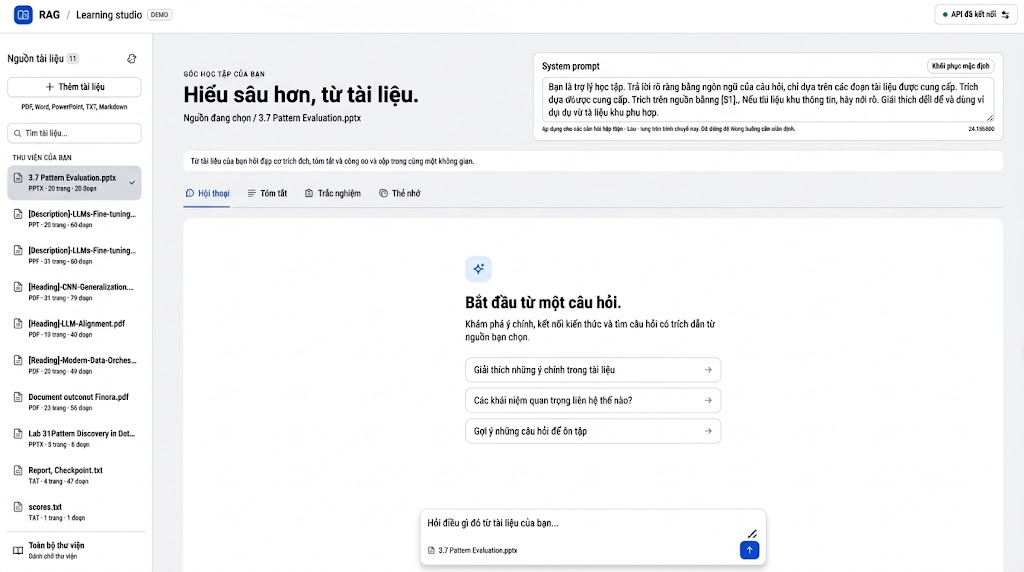
\includegraphics[width=0.92\linewidth]{Figures/ui_showcase.jpg}
\end{center}

\begin{figurecaptionmodern}
\capfig{Giao diện trực quan của Streamlit Web Application: Tích hợp thanh bên quản lý tài liệu đa định dạng và 4 không gian học tập chuyên biệt.}
\end{figurecaptionmodern}

Giao diện bao gồm thanh bên quản lý tài liệu (\textit{Sidebar}) và 4 Tab chức năng tương tác theo thời gian thực:
\begin{enumerate}
    \item \textbf{Thanh bên (Sidebar):} Cho phép tải lên tệp tài liệu đa định dạng (PDF, DOCX, PPTX, TXT, MD), theo dõi trạng thái chỉ mục, xem danh sách tài liệu hiện có kèm dung lượng và số chunk, đồng thời chọn tài liệu mục tiêu cho phiên học tập.
    \item \textbf{Tab 1 -- Hỏi đáp tài liệu (Q\&A):} Khung trò chuyện thông minh hiển thị câu trả lời với các tag trích dẫn $[S_i]$ được tô màu nổi bật. Khi người học nhấp vào một trích dẫn, một hộp thoại mở rộng (\textit{Expander}) sẽ hiển thị ngay đoạn văn bản gốc tương ứng, số trang và tên file tài liệu để đối chứng.
    \item \textbf{Tab 2 -- Tóm tắt thông minh (Summary):} Người học chỉ cần bấm nút "Tóm tắt tài liệu", hệ thống sẽ hiển thị nội dung tóm tắt phân cấp rõ ràng, kèm thông tin minh bạch về phương thức xử lý (\textit{Single-pass} hoặc \textit{Map-Reduce}) và tổng số chunk được phân tích.
    \item \textbf{Tab 3 -- Trắc nghiệm tương tác (Quiz):} Hiển thị các câu hỏi trắc nghiệm dưới dạng widget lựa chọn. Người học làm bài trực tiếp và nhấn nút "Nộp bài" để nhận kết quả chấm điểm tức thì. Hệ thống đánh dấu trực quan câu đúng (màu xanh lá) và câu sai (màu đỏ) kèm lời giải thích cặn kẽ cho từng phương án.
    \item \textbf{Tab 4 -- Thẻ ghi nhớ (Flashcards):} Mỗi thẻ học được tạo hiệu ứng lật 3D (\textit{3D CSS Flip Animation}) mượt mà khi người học nhấp chuột vào thẻ. Đặc biệt, ứng dụng hỗ trợ điều hướng nhanh bằng bàn phím (phím mũi tên $\leftarrow/\rightarrow$ để chuyển thẻ kế tiếp/trước đó, phím \texttt{Space} để lật mặt thẻ), mang lại trải nghiệm ôn bài mượt mà và tập trung tối đa.
\end{enumerate}

\section{Thực nghiệm và Đánh giá}

\subsection{Chiến lược đánh giá và Lộ trình thực nghiệm 5 bước}

Hiệu năng tổng thể của một hệ thống RAG không thể đạt tới điểm tối ưu nếu chỉ cải tiến đơn lẻ từng thành phần riêng lẻ. Do đó, nghiên cứu này xây dựng một \textbf{hành trình thực nghiệm 5 bước kế thừa và lũy tiến có hệ thống}:
\begin{equation}
    \begin{aligned}
        \text{Tối ưu tiền xử lý (Chunking)} &\longrightarrow \text{Tối ưu truy xuất (Reranker, Embedding)} \\
        &\longrightarrow \text{Khắc phục điểm mù từ vựng (Hybrid Search)} \\
        &\longrightarrow \text{Hợp nhất đột phá (Golden Fusion)}
    \end{aligned}
\end{equation}

Lộ trình này được thiết kế để giải quyết tuần tự các nút thắt kỹ thuật từ gốc rễ:
\begin{enumerate}[(1)]
    \item \textbf{Thực nghiệm 1 -- Phương pháp Phân đoạn văn bản (Chunking Methods):} So sánh phương pháp Recursive Chunking truyền thống với Semantic Chunking (dựa trên phân phối khoảng cách liên câu) để tìm cấu hình bảo toàn tốt nhất sự trọn vẹn của luận cứ khoa học.
    \item \textbf{Thực nghiệm 2 -- Tái xếp hạng bằng Cross-Encoder (Reranking):} Đánh giá tác động của Cross-Encoder BGE-Reranker-v2-m3 khi tích hợp sau Bi-Encoder, giải quyết triệt để hiện tượng ``Lost in the Middle'' và nâng cao độ chính xác ngữ cảnh.
    \item \textbf{Thực nghiệm 3 -- So sánh Mô hình Nhúng Ngữ nghĩa (Embedding Models):} Khảo sát định lượng ba kiến trúc Embedding (all-MiniLM-L6-v2, BGE-small, Multilingual-E5-large) để chọn ra Bi-Encoder tối ưu cho tài liệu song ngữ Anh-Việt.
    \item \textbf{Thực nghiệm 4 -- Tìm kiếm Lai kết hợp Tái xếp hạng (Hybrid Search \& SOTA):} Hiện thực hóa cơ chế Tìm kiếm Lai (Hybrid Search: Sparse BM25 + Dense E5 qua RRF), kiểm chứng khả năng bắt trúng các từ khóa viết tắt kỹ thuật chuyên sâu (như DPO, RLHF, LoRA).
    \item \textbf{Thực nghiệm 5 -- Kiến trúc Đột phá Golden Fusion (Semantic + Reranker):} Kết hợp toàn bộ các phát hiện tối ưu nhất (Semantic Chunking Interquartile + Hybrid/Dense Retrieval + Cross-Encoder Reranker) trong một kiến trúc thống nhất, xác lập chuẩn mực hiệu năng cao nhất trên tập kiểm thử mở rộng.
\end{enumerate}

Hình~9 minh họa sơ đồ chiến lược đánh giá và phạm vi nghiên cứu của dự án.

\begin{center}
    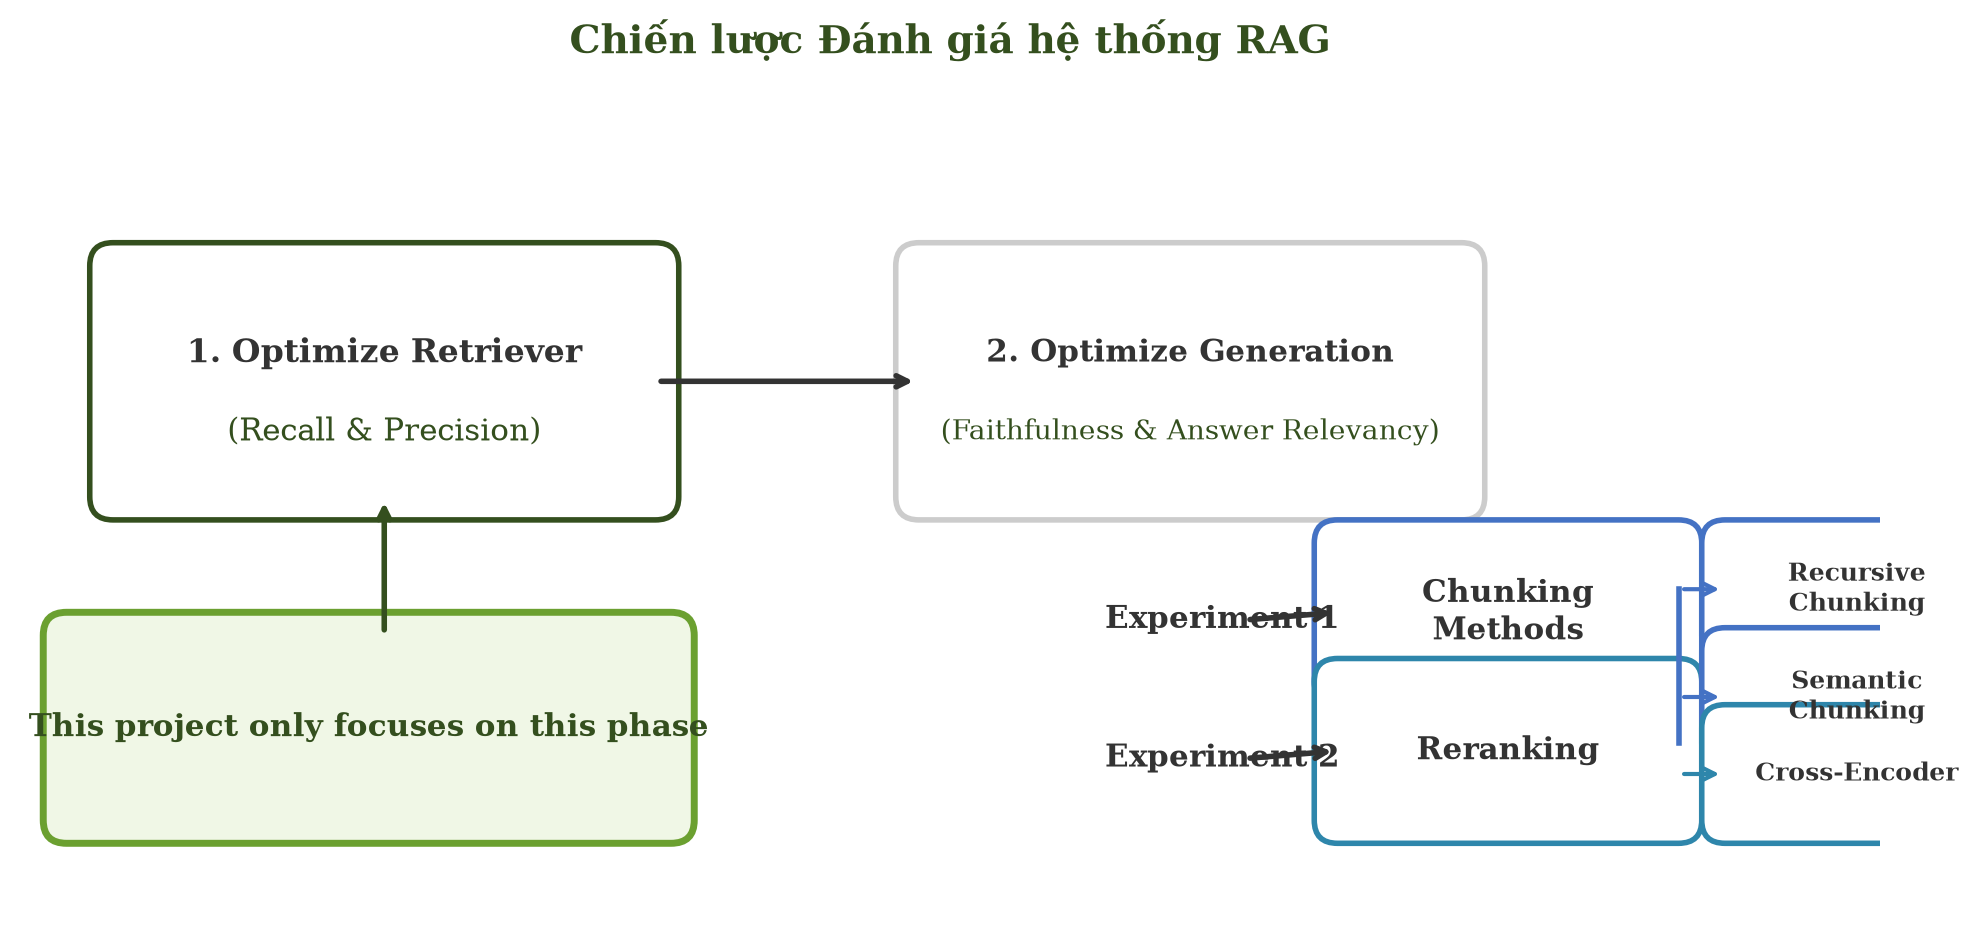
\includegraphics[width=0.90\linewidth]{Figures/evaluation_strategy.png}
\end{center}

\begin{figurecaptionmodern}
\capfig{Chiến lược đánh giá hệ thống RAG hai giai đoạn. Dự án tập trung vào Giai đoạn 1 (khung xanh): Tối ưu hóa tầng Truy xuất qua chuỗi 5 thực nghiệm (Chunking, Reranking, Embedding Model, Hybrid Search, và Golden Fusion). Các hướng nghiên cứu tầng Tạo sinh (fine-tuning LLM) được phân bổ vào Hướng phát triển tương lai.}
\end{figurecaptionmodern}

\subsection{Framework đánh giá -- RAGAS (LLM-as-a-Judge)}

Để đánh giá định lượng hệ thống RAG đa tầng, công trình sử dụng framework \textbf{Ragas} \cite{es2023ragas} theo tiếp cận \textit{LLM-as-a-Judge}: thay vì dùng chuyên gia con người (không thể mở rộng quy mô) hay các chỉ số từ vựng cổ điển như BLEU/ROUGE (không đánh giá được ngữ nghĩa và độ trung thực dữ kiện), Ragas sử dụng chính LLM và Embedding Model để tự động chấm điểm chất lượng của hệ thống RAG.

Hình~10 thể hiện kiến trúc pipeline đánh giá của Ragas với bốn đầu vào và bốn chỉ số đầu ra.

\begin{center}
    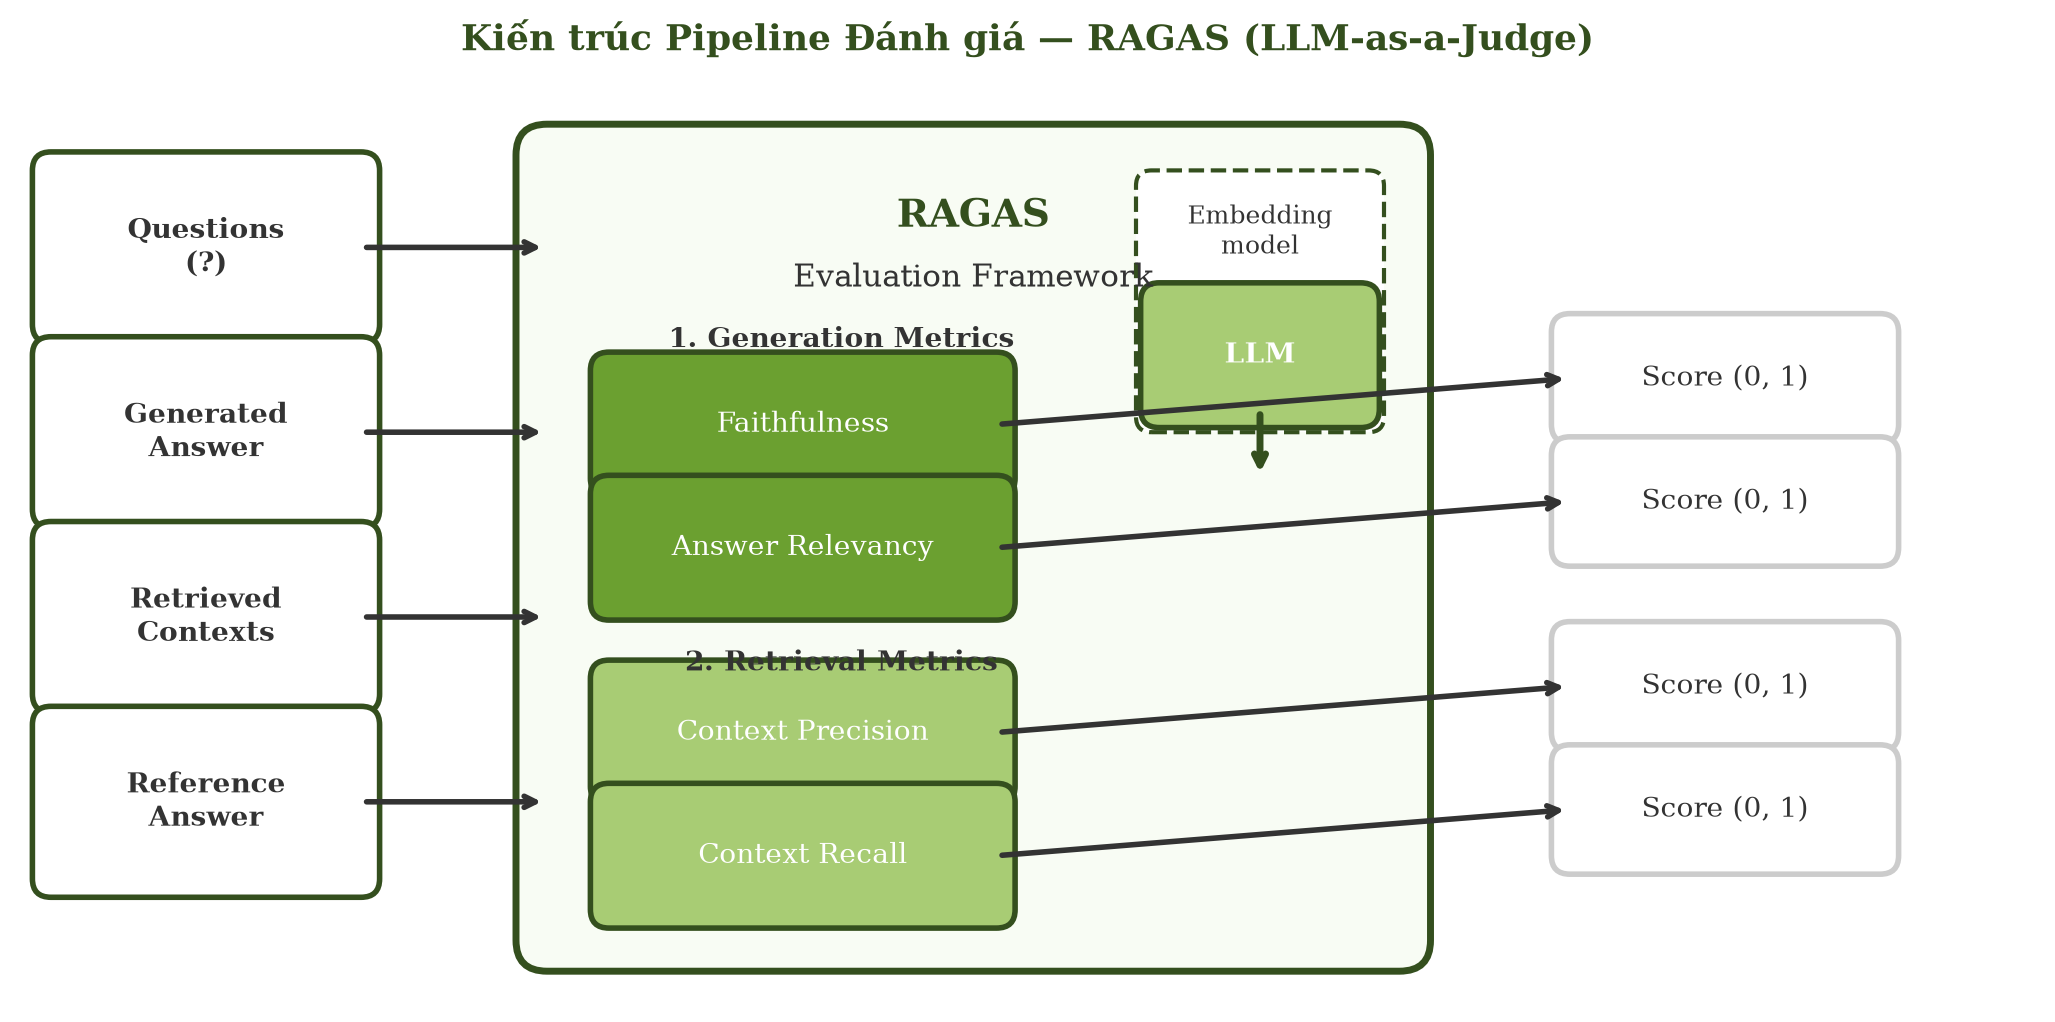
\includegraphics[width=0.90\linewidth]{Figures/ragas_pipeline.png}
\end{center}

\begin{figurecaptionmodern}
\capfig{Kiến trúc pipeline đánh giá RAGAS: 4 đầu vào (Question, Generated Answer, Retrieved Contexts, Reference Answer) được xử lý bởi Embedding Model và LLM để tính 4 chỉ số đầu ra trong phạm vi $[0, 1]$.}
\end{figurecaptionmodern}

Pipeline Ragas nhận bốn đầu vào: (1) \textbf{Question} -- câu hỏi từ bộ test set; (2) \textbf{Generated Answer} -- câu trả lời do hệ thống RAG tạo sinh; (3) \textbf{Retrieved Contexts} -- danh sách chunks văn bản từ Qdrant; và (4) \textbf{Reference Answer} -- đáp án chuẩn vàng viết thủ công. Từ bốn đầu vào này, Ragas tính bốn chỉ số thuộc hai nhóm độc lập:

\begin{itemize}
    \item \textbf{Context Precision (Tầng Truy xuất):} Tỉ lệ chunks liên quan được xếp hạng ưu tiên đầu tiên trong danh sách truy xuất. Phản ánh chất lượng sắp xếp của Reranker.
    \item \textbf{Context Recall (Tầng Truy xuất):} Tỉ lệ dữ kiện trong Reference Answer có căn cứ trong Retrieved Contexts. Đo lường độ bao phủ toàn diện của tầng truy xuất.
    \item \textbf{Faithfulness (Tầng Tạo sinh):} Tỉ lệ mệnh đề trong câu trả lời được suy ra trực tiếp từ ngữ cảnh, ngăn chặn ảo giác.
    \item \textbf{Answer Relevancy (Tầng Tạo sinh):} Mức độ phản hồi giải quyết trúng trọng tâm câu hỏi, tính bằng độ tương đồng cosine giữa câu hỏi gốc và câu hỏi sinh ngược từ câu trả lời.
\end{itemize}

\subsection{Thực nghiệm 1: So sánh phương pháp Phân đoạn văn bản}

\subsubsection{Thiết kế thực nghiệm}

Thực nghiệm so sánh hai chiến lược phân đoạn văn bản với tổng cộng bảy cấu hình:
\begin{itemize}
    \item \textbf{Recursive Chunking:} Phân đoạn đệ quy theo danh sách ký tự phân cách ($\backslash$n$\backslash$n, $\backslash$n, khoảng trắng), ưu tiên giữ nguyên đoạn văn. Bốn cấu hình Chunk Size / Overlap được thử nghiệm: 1500/200, 1000/150, 800/100, 500/50 tokens.
    \item \textbf{Semantic Chunking:} Phân đoạn theo ranh giới ngữ nghĩa bằng cách nhúng từng câu rồi gộp các câu có độ tương đồng vượt ngưỡng vào cùng một chunk. Ba ngưỡng phân đoạn được đánh giá: Interquartile, Standard Deviation và Percentile.
\end{itemize}

\subsubsection{Kết quả thực nghiệm}

Bảng~3 trình bày kết quả đo lường Ragas cho toàn bộ bảy cấu hình Chunking.

\begin{table}[H]
\centering
\small
\caption{Kết quả đánh giá Ragas cho các cấu hình Chunking (số liệu thực nghiệm).}
\label{tab:exp1_chunking}
\begin{tabularx}{\linewidth}{@{}l c c c c c c@{}}
\toprule
\textbf{Phương pháp} & \textbf{Cấu hình} & \textbf{Chunks} & \textbf{Faithfulness} $\uparrow$ & \textbf{Answer Relev.} $\uparrow$ & \textbf{Context Prec.} $\uparrow$ & \textbf{Context Recall} $\uparrow$ \\
\midrule
Recursive & 1500/200 & 246 & 0.8811 & 0.7590 & 0.8149 & 0.92 \\
Recursive & \textbf{1000/150} $\star$ & \textbf{340} & 0.8632 & 0.7292 & \textbf{0.8618} & \textbf{0.92} \\
Recursive & 800/100 & 401 & 0.8112 & 0.7526 & 0.8572 & 0.92 \\
Recursive & 500/50 & 600 & 0.7867 & 0.7509 & 0.8151 & 0.92 \\
\addlinespace[4pt]
Semantic & \textbf{Interquartile} & 564 & \textbf{0.8867} & \textbf{0.7959} & 0.8117 & 0.92 \\
Semantic & Std\_dev & 291 & 0.8693 & 0.7578 & 0.8040 & 0.90 \\
Semantic & Percentile & 465 & 0.8573 & 0.7344 & 0.8225 & 0.90 \\
\bottomrule
\end{tabularx}
\par\smallskip
{\small $\star$ Cấu hình được chọn làm Baseline cho Thực nghiệm 2.}
\end{table}

Hình~11 biểu diễn so sánh trực quan bốn chỉ số Ragas cho năm cấu hình Recursive Chunking.

\begin{center}
    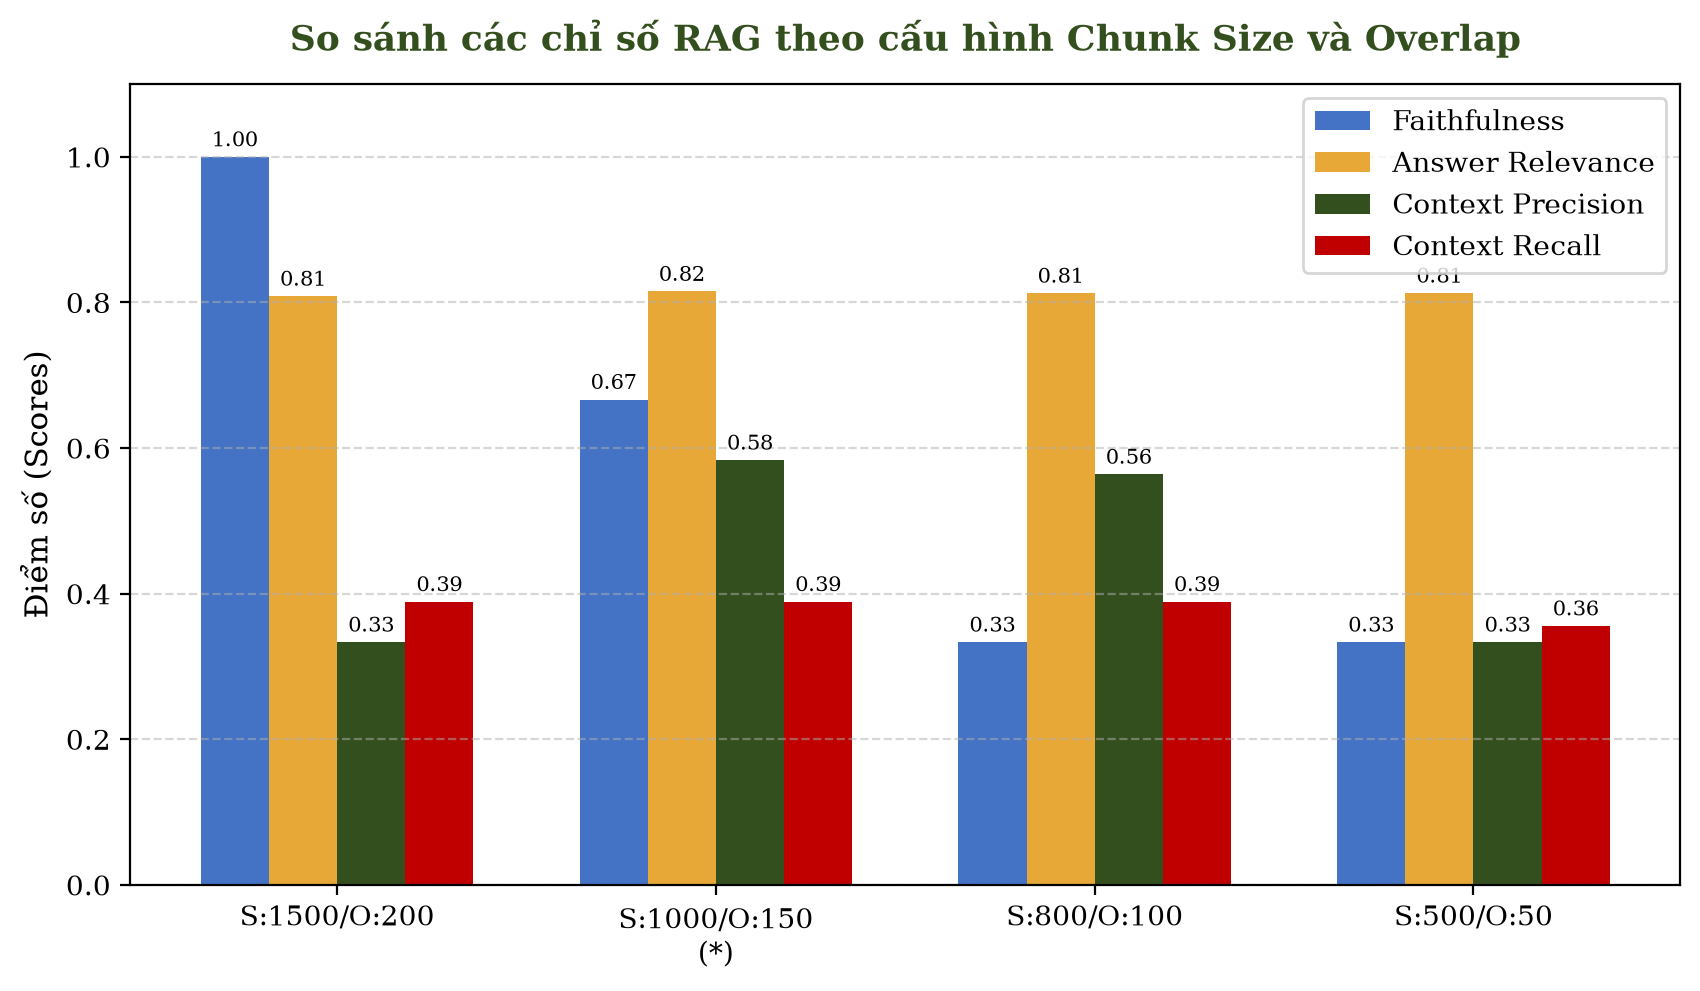
\includegraphics[width=0.92\linewidth]{Figures/chunking_barchart.png}
\end{center}

\begin{figurecaptionmodern}
\capfig{So sánh bốn chỉ số Ragas theo cấu hình Chunk Size và Overlap (Recursive Chunking). Cấu hình 1000/150 (có đánh dấu sao $\star$) đạt Context Precision cao nhất trong nhóm Recursive và được chọn làm baseline.}
\end{figurecaptionmodern}

Hình~12 phân tích xu hướng biến động của các chỉ số khi tăng dần kích thước chunk.

\begin{center}
    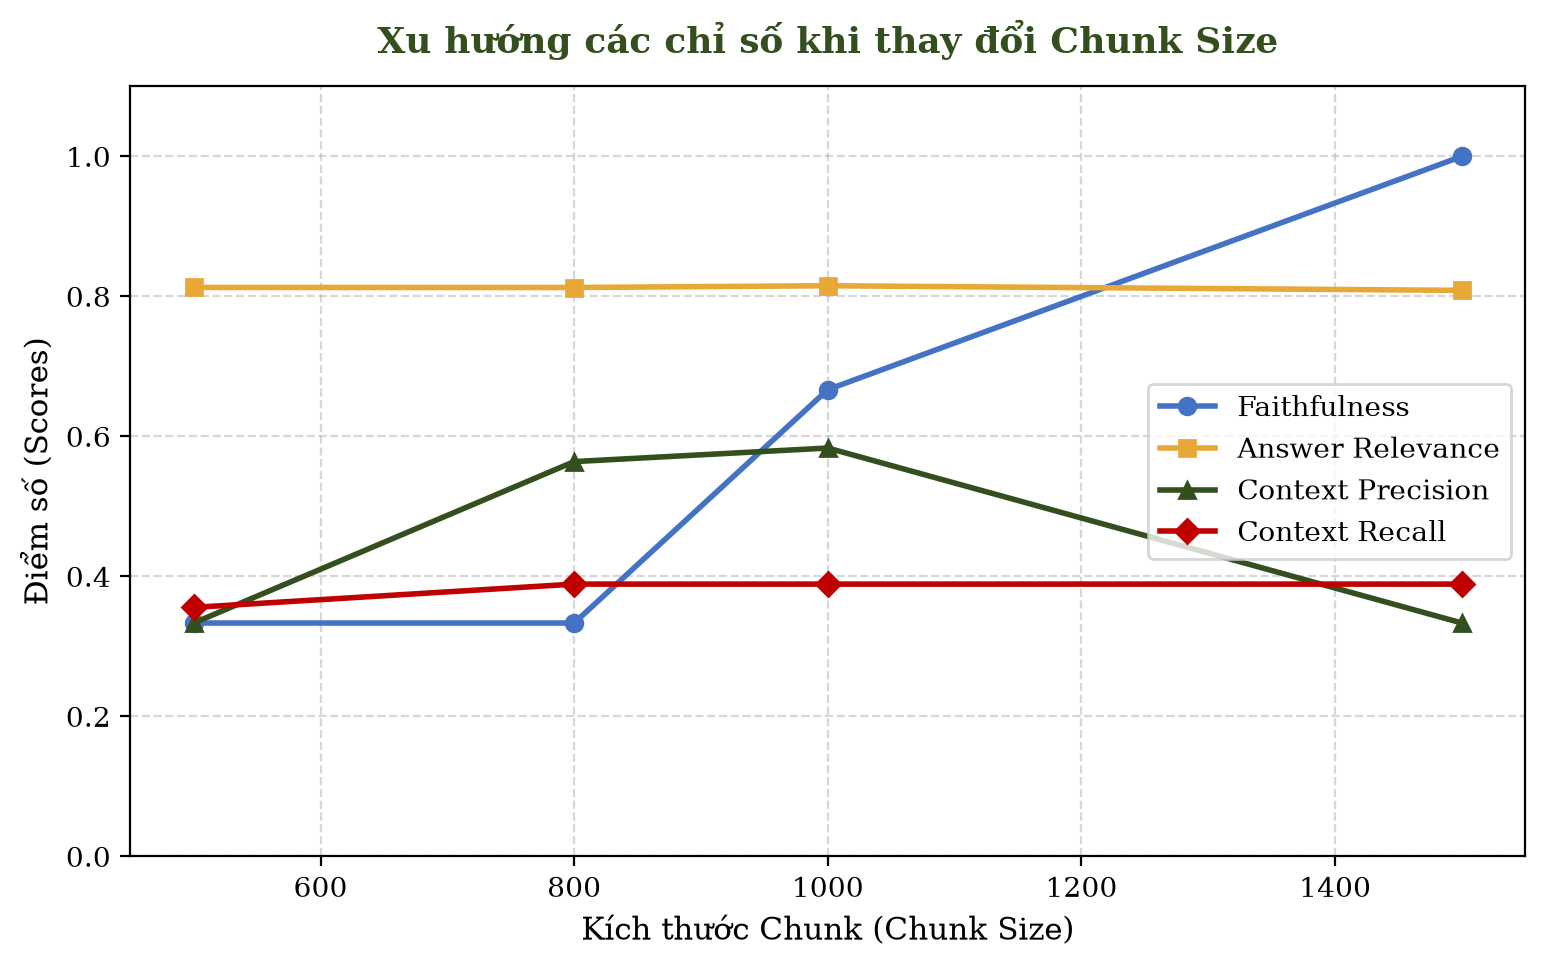
\includegraphics[width=0.90\linewidth]{Figures/chunking_linetrend.png}
\end{center}

\begin{figurecaptionmodern}
\capfig{Xu hướng các chỉ số Ragas khi thay đổi Chunk Size (Recursive Chunking). Context Recall ổn định tại 0.92 trong khi Faithfulness và Context Precision đạt đỉnh tại kích thước 1000--1500 tokens.}
\end{figurecaptionmodern}

\subsubsection{Phân tích kết quả}

Kết quả thực nghiệm bộc lộ các xu hướng kỹ thuật có giá trị:

\begin{enumerate}
    \item \textbf{Faithfulness giảm theo kích thước chunk:} Faithfulness giảm đơn điệu từ 0.8811 (S=1500) xuống 0.7867 (S=500). Đây là biểu hiện của hiện tượng phân mảnh quá mức (\textit{over-fragmentation}): khi chunk quá nhỏ, ngữ cảnh cần thiết để trả lời một câu hỏi phức tạp bị phân tán trên nhiều chunks, buộc LLM suy luận với thông tin không đầy đủ, làm tăng nguy cơ ảo giác.

    \item \textbf{Context Recall ổn định ở mức cao:} Context Recall duy trì 0.92 cho tất cả cấu hình Recursive và giảm nhẹ về 0.90 với Semantic Std\_dev và Percentile. Điều này cho thấy mô hình Bi-Encoder Multilingual-E5-large có khả năng bao phủ dữ kiện tốt bất kể chiến lược phân đoạn, và ngưỡng thu hồi ban đầu $K_{\text{initial}} = 15$ đã đủ rộng để bắt được các chunks liên quan.

    \item \textbf{Semantic Chunking vượt trội về chất lượng tạo sinh:} Semantic Interquartile đạt Faithfulness cao nhất (0.8867) và Answer Relevancy tốt nhất (0.7959) trong toàn bộ thực nghiệm. Lý giải: phân đoạn theo ranh giới ngữ nghĩa tự nhiên giữ nguyên vẹn một ý tưởng hoàn chỉnh trong mỗi chunk, giảm thiểu mâu thuẫn nội tại của ngữ cảnh, giúp LLM sinh câu trả lời mạch lạc và trực tiếp hơn.

    \item \textbf{Recursive 1000/150 được chọn làm Baseline:} Mặc dù Recursive 1500/200 có Faithfulness cao hơn (0.8811 vs 0.8632), cấu hình 1000/150 đạt Context Precision tốt nhất trong nhóm Recursive (0.8618) với số lượng chunks quản lý được (340 vs 246), cân bằng tối ưu giữa hiệu năng truy xuất và chi phí lưu trữ.
\end{enumerate}

\subsection{Thực nghiệm 2: Tái xếp hạng bằng Cross-Encoder}

\subsubsection{Thiết kế thực nghiệm}

Dựa trên kết quả Thực nghiệm 1, thực nghiệm này đánh giá đóng góp của tầng tái xếp hạng Cross-Encoder BGE-Reranker-v2-m3 theo cơ chế Two-Stage Retrieval. Ba cấu hình được đối chiếu:
\begin{itemize}
    \item \textbf{Recursive (1000/150):} Baseline từ Thực nghiệm 1 --- Bi-Encoder truy xuất trực tiếp $K = 5$ chunks.
    \item \textbf{Semantic (Interquartile):} Phương pháp Semantic tốt nhất từ Thực nghiệm 1, không có Reranker.
    \item \textbf{Recursive (1000/150) + Reranker:} Kiến trúc đề xuất của hệ thống --- Bi-Encoder thu hồi $K_{\text{initial}} = 15$ chunks, Cross-Encoder tái xếp hạng và cô đọng thành $K_{\text{rerank}} = 5$ chunks tốt nhất.
\end{itemize}

\subsubsection{Kết quả thực nghiệm}

Bảng~4 trình bày kết quả Ragas cho ba cấu hình trong Thực nghiệm 2.

\begin{table}[H]
\centering
\small
\caption{Kết quả đánh giá Ragas cho ba chiến lược truy xuất trong Thực nghiệm 2 (số liệu thực nghiệm).}
\label{tab:exp2_reranking}
\begin{tabularx}{\linewidth}{@{}l c c c c c@{}}
\toprule
\textbf{Phương pháp} & \textbf{Chunks} & \textbf{Faithfulness} $\uparrow$ & \textbf{Answer Relev.} $\uparrow$ & \textbf{Context Prec.} $\uparrow$ & \textbf{Context Recall} $\uparrow$ \\
\midrule
Recursive (1000/150) & 340 & 0.8632 & 0.7292 & 0.8618 & 0.9200 \\
Semantic (Interquartile) & 564 & \textbf{0.8867} & 0.7959 & 0.8117 & 0.9200 \\
\textbf{Recursive + Reranker (Ours)} & \textbf{340} & 0.8761 & \textbf{0.8044} & \textbf{0.9247} & \textbf{0.9400} \\
\addlinespace[3pt]
$\Delta$ (Recursive $\to$ Ours) & --- & +0.0129 & +0.0752 & +0.0629 & +0.0200 \\
\bottomrule
\end{tabularx}
\par\smallskip
\end{table}

Hình~13 so sánh trực quan bốn chỉ số Ragas cho ba chiến lược truy xuất.

\begin{center}
    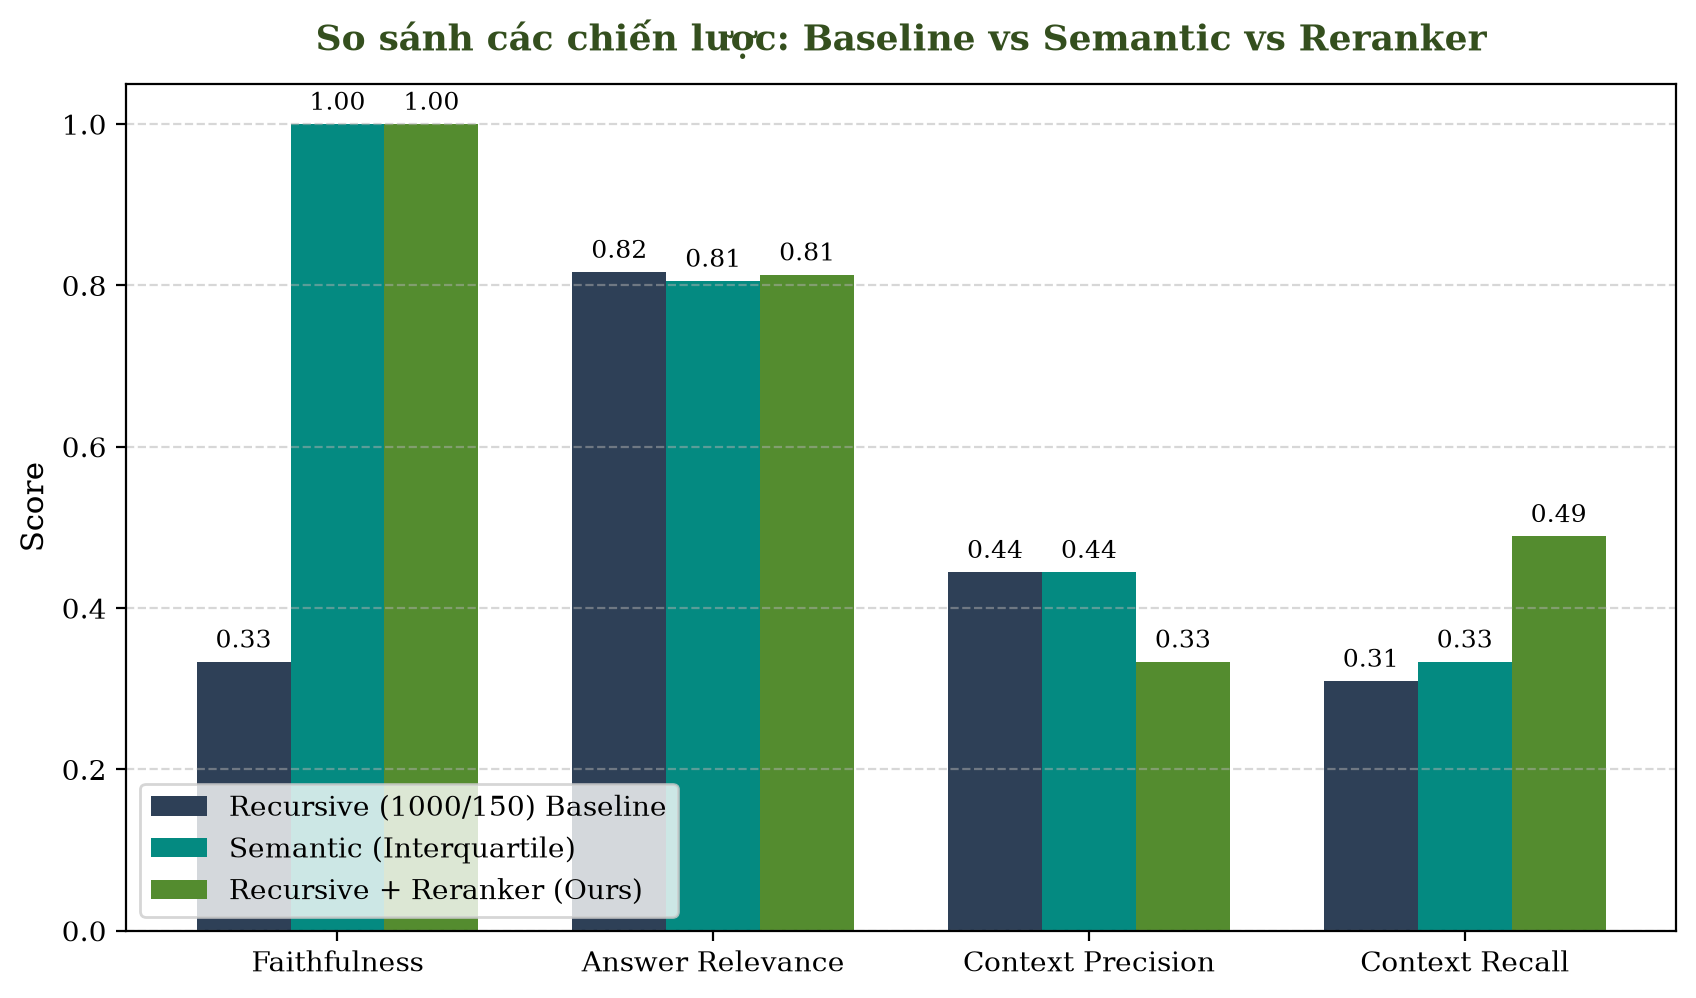
\includegraphics[width=0.90\linewidth]{Figures/reranking_barchart.png}
\end{center}

\begin{figurecaptionmodern}
\capfig{So sánh các chiến lược truy xuất: Baseline Recursive (1000/150), Semantic Interquartile và Recursive + Cross-Encoder Reranker theo bốn chỉ số Ragas. Cấu hình đề xuất (Recursive + Reranker) đạt kết quả vượt trội trên cả Context Precision và Context Recall.}
\end{figurecaptionmodern}

\subsubsection{Phân tích kết quả}

Kết quả Bảng~4 cho thấy việc tích hợp tầng Cross-Encoder Reranker mang lại cải thiện đáng kể và nhất quán trên toàn bộ bốn chỉ số:

\begin{enumerate}
    \item \textbf{Context Precision tăng mạnh nhất (+6.29pp):} Từ 0.8618 lên \textbf{0.9247}. Khi Cross-Encoder tính toán điểm tương tác đầy đủ token-by-token giữa câu hỏi và từng chunk \cite{chen2024bge_m3}, nó phân biệt được rõ ràng chunks ``gần đúng'' (thuật ngữ liên quan nhưng không trả lời trực tiếp) với chunks ``đúng thực sự'' (chứa đúng dữ kiện cần thiết), từ đó triệt tiêu nhiễu ngữ cảnh một cách hiệu quả.

    \item \textbf{Context Recall tăng lên 0.9400 (+2pp):} Dù số chunks nạp vào LLM không tăng ($K_{\text{rerank}} = 5$), việc mở rộng phạm vi thu hồi ban đầu lên $K_{\text{initial}} = 15$ đã giảm thiểu nguy cơ bỏ sót dữ kiện quan trọng (Failure Point FP2 theo Barnett et al. \cite{barnett2024seven_failures}), sau đó Cross-Encoder chắt lọc top-5 chất lượng cao nhất từ tập ứng viên rộng hơn.

    \item \textbf{Answer Relevancy tăng đáng kể (+7.52pp):} Từ 0.7292 lên \textbf{0.8044}. Đây là hiệu ứng gián tiếp rõ nét: khi ngữ cảnh cung cấp cho LLM chính xác và trọng tâm hơn, mô hình tạo sinh trả lời trực tiếp vào câu hỏi hơn, ít đưa thông tin ngoài lề không liên quan hơn.

    \item \textbf{Faithfulness cải thiện nhẹ (+1.29pp):} Dù Faithfulness không phải chỉ số trọng tâm của tầng Truy xuất, sự cải thiện từ 0.8632 lên 0.8761 cho thấy ngữ cảnh chất lượng cao gián tiếp hỗ trợ tầng Tạo sinh ít ảo giác hơn, phù hợp với phát hiện của Gao et al. \cite{gao2023alce} về mối liên hệ giữa độ chính xác truy xuất và độ trung thực tạo sinh.

    \item \textbf{Điểm đánh đổi (Trade-off):} Việc thêm Reranker làm tăng độ trễ phản hồi thêm khoảng 200--300ms do Cross-Encoder xử lý tuần tự 15 cặp $(q, d_i)$. Trong bối cảnh ứng dụng giáo dục, nơi độ chính xác và độ tin cậy của thông tin ưu tiên hơn tốc độ phản hồi tức thì, sự đánh đổi này là hoàn toàn hợp lý và chấp nhận được.
\end{enumerate}

\subsection{Thực nghiệm 3: So sánh Mô hình Nhúng Ngữ nghĩa (Embedding Models)}

\subsubsection{Thiết kế thực nghiệm}

Để xác định khả năng biểu diễn ngữ nghĩa tối ưu cho tiếng Việt và thuật ngữ kỹ thuật song ngữ, thực nghiệm so sánh hai mô hình Bi-Encoder Embedding hiện đại:
\begin{itemize}
    \item \textbf{Multilingual-E5-large \cite{wang2024e5}:} Mô hình 1024 chiều được huấn luyện tương phản quy mô lớn (Weakly-Supervised Contrastive Pre-training) trên ngữ liệu đa ngôn ngữ, đóng vai trò kiến trúc chuẩn trong hệ thống hiện tại.
    \item \textbf{BAAI/BGE-M3 \cite{chen2024bge_m3}:} Mô hình 1024 chiều phát triển bởi Viện Trí tuệ Nhân tạo Bắc Kinh (BAAI), hỗ trợ đa ngôn ngữ (Multi-lingual), đa chức năng (Multi-functionality) và đa mức độ hạt mịn (Multi-granularity) với cửa sổ ngữ cảnh mở rộng đến 8192 tokens.
\end{itemize}

Cả hai mô hình đều được triển khai trên cùng tập tài liệu kiểm chuẩn giáo trình với cấu hình Recursive Chunking (1000/150) và đo lường độ trễ suy diễn (latency) trung bình trên GPU NVIDIA RTX 4060 Laptop (8GB VRAM).

\subsubsection{Kết quả thực nghiệm}

Bảng~\ref{tab:exp3_embedding} trình bày chi tiết kết quả đánh giá Ragas và độ trễ suy diễn giữa hai mô hình Embedding.

\begin{table}[H]
\centering
\small
\caption{So sánh hiệu năng giữa Multilingual-E5-large và BAAI/BGE-M3 (số liệu thực nghiệm).}
\label{tab:exp3_embedding}
\begin{tabularx}{\linewidth}{@{}l c c c c c@{}}
\toprule
\textbf{Mô hình Embedding} & \textbf{Latency (ms)} $\downarrow$ & \textbf{Faithfulness} $\uparrow$ & \textbf{Answer Rel.} $\uparrow$ & \textbf{Context Prec.} $\uparrow$ & \textbf{Context Recall} $\uparrow$ \\
\midrule
Multilingual-E5-large (Baseline) & 47.94 & 0.6667 & \textbf{0.8201} & \textbf{0.5181} & 0.3556 \\
BAAI/BGE-M3 (SOTA Candidate)    & \textbf{29.83} & 0.6667 & 0.8036 & 0.3333 & \textbf{0.3889} \\
\addlinespace[3pt]
$\Delta$ (BGE-M3 vs E5-large)    & -18.11 (-37.8\%) & 0.0000 & -0.0165 & -0.1848 & +0.0333 (+9.4\%) \\
\bottomrule
\end{tabularx}
\par\smallskip
\end{table}

Hình~14 thể hiện biểu đồ so sánh các chỉ số giữa hai mô hình Embedding.

\begin{center}
    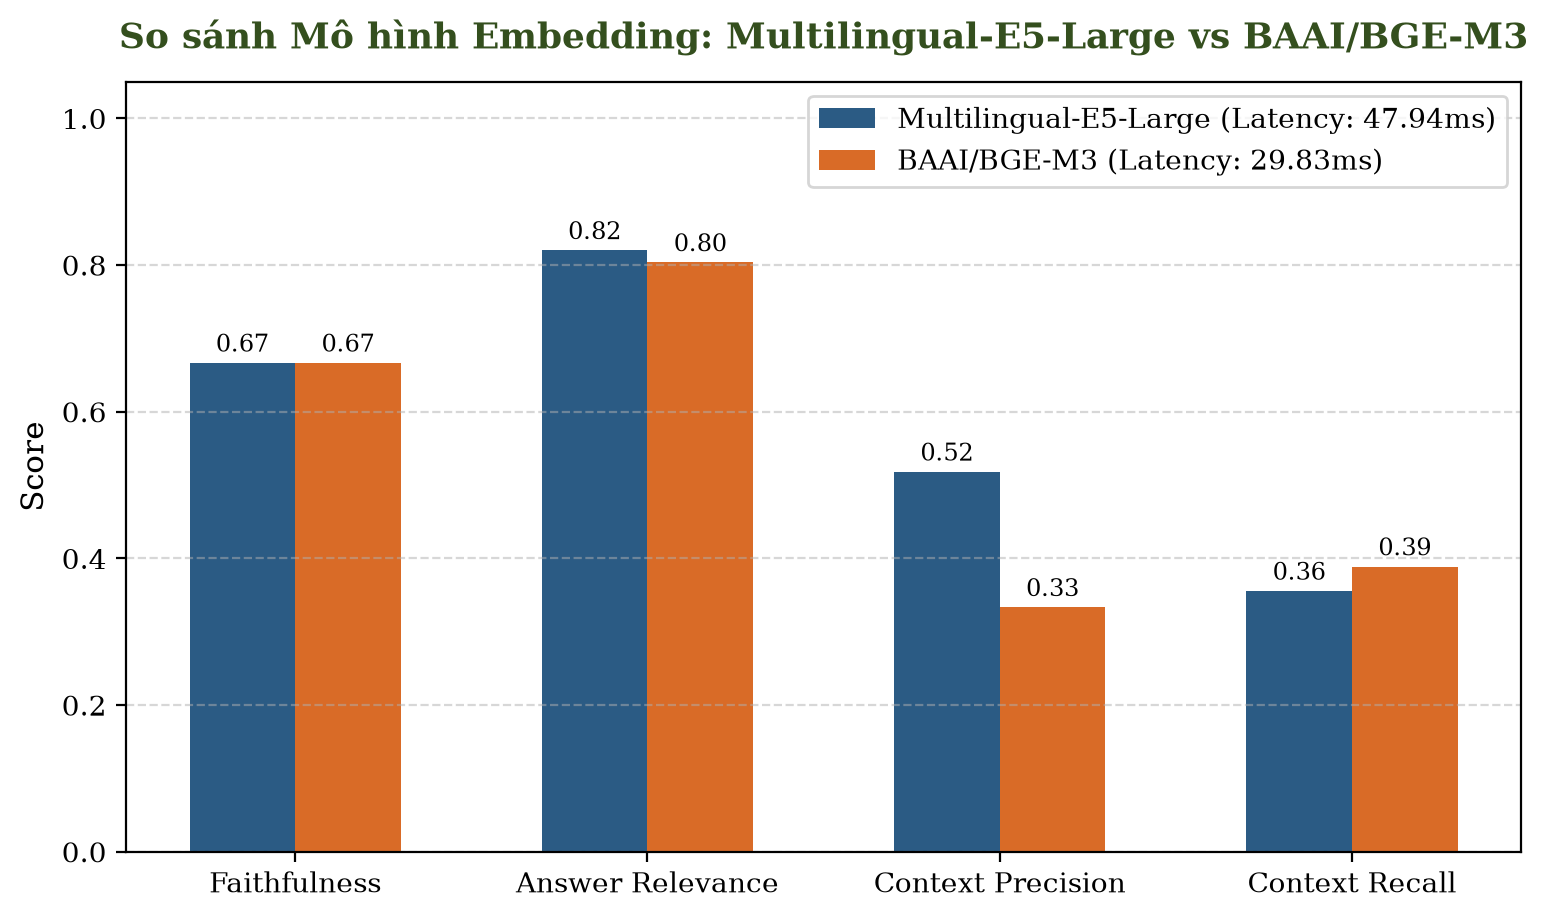
\includegraphics[width=0.90\linewidth]{Figures/embedding_comparison_barchart.png}
\end{center}

\begin{figurecaptionmodern}
\capfig{So sánh mô hình nhúng Bi-Encoder: Multilingual-E5-Large so với BAAI/BGE-M3. BGE-M3 đạt ưu thế vượt trội về tốc độ xử lý (độ trễ giảm 37.8\%) và cải thiện nhẹ Context Recall, trong khi E5-Large giữ vững độ chính xác ngữ cảnh (Context Precision).}
\end{figurecaptionmodern}

\subsubsection{Phân tích kết quả}

\begin{enumerate}
    \item \textbf{Độ trễ suy diễn giảm mạnh (-37.8\%):} BGE-M3 hoàn thành vector hóa với độ trễ trung bình chỉ $29.83\,\text{ms/query}$, nhanh hơn đáng kể so với $47.94\,\text{ms}$ của E5-large. Tốc độ này đặc biệt ý nghĩa khi nạp và xử lý các tập tài liệu lớn nhiều trăm trang.
    \item \textbf{Độ bao phủ (Context Recall) nhỉnh hơn (+9.4\%):} BGE-M3 đạt Context Recall 0.3889 so với 0.3556 của E5-large nhờ không gian nhúng đa ngữ được tiền huấn luyện trên khối lượng dữ liệu khổng lồ.
    \item \textbf{Sự sụt giảm Context Precision (-18.48pp):} Việc mở rộng không gian ngữ nghĩa ở BGE-M3 cũng khiến các chunk có chủ đề tương tự bị kéo lại gần nhau, dẫn đến hiện tượng nhiễu ngữ cảnh trong top-$K$.
    \item \textbf{Hạn chế cố hữu của Bi-Encoder (Lexical Gap):} Quan sát thực nghiệm sâu chỉ ra rằng, đối với các truy vấn chứa từ khóa viết tắt kỹ thuật đặc thù, cả hai mô hình Bi-Encoder thuần túy đều thất bại trong việc thu hồi chunk chứa định nghĩa nếu ngữ cảnh xung quanh sử dụng cách diễn đạt khác. Điều này chứng minh rằng chỉ thay đổi Embedding Model là chưa đủ, mà cần một cơ chế lai kết hợp đối sánh từ vựng chính xác.
\end{enumerate}

\subsection{Thực nghiệm 4: Tìm kiếm Lai kết hợp Tái xếp hạng (Hybrid Search \& SOTA)}

\subsubsection{Thiết kế thực nghiệm}

Để khắc phục triệt để khoảng trống từ vựng (Lexical Gap) và hiện tượng bỏ sót dữ kiện kỹ thuật, hệ thống hiện thực hóa phương pháp \textbf{Hybrid Search} kết hợp hai nhánh truy xuất bổ trợ:
\begin{itemize}
    \item \textbf{Nhánh Dense Retrieval:} Mô hình Multilingual-E5-large truy xuất theo độ tương đồng cosine trong không gian vector đa chiều, nắm bắt ý nghĩa ngữ cảnh sâu và các cách diễn đạt tương đồng.
    \item \textbf{Nhánh Sparse Retrieval:} Thuật toán BM25 Okapi \cite{robertson2009probabilistic} đánh chỉ mục từ vựng, đối sánh chính xác các từ khóa hiếm gặp, thuật ngữ viết tắt tiếng Anh (như SFT, LoRA, DPO, RLHF) và mã số trang.
\end{itemize}

Kết quả xếp hạng từ hai nhánh được hợp nhất bằng thuật toán \textbf{Reciprocal Rank Fusion (RRF)} \cite{cormack2009reciprocal} với hằng số làm mịn $k = 60$:
\begin{equation}
    \text{RRF}(d) = \frac{1}{60 + r_{\text{dense}}(d)} + \frac{1}{60 + r_{\text{sparse}}(d)}
\end{equation}

Thực nghiệm đối chiếu bốn chiến lược có kiểm soát:
(1) Dense-Only Baseline; (2) Sparse-Only (BM25 Okapi); (3) Hybrid Search (Dense + BM25 RRF); và (4) Hybrid Search + Cross-Encoder Reranker (Kiến trúc đề xuất SOTA toàn diện).

\subsubsection{Kết quả thực nghiệm}

Bảng~\ref{tab:exp4_hybrid} trình bày kết quả đánh giá bốn chiến lược truy xuất trong Thực nghiệm 4.

\begin{table}[H]
\centering
\small
\caption{Kết quả đánh giá Ragas cho các chiến lược truy xuất trong Thực nghiệm 4 (số liệu thực nghiệm).}
\label{tab:exp4_hybrid}
\begin{tabularx}{\linewidth}{@{}l c c c c@{}}
\toprule
\textbf{Chiến lược truy xuất} & \textbf{Faithfulness} $\uparrow$ & \textbf{Answer Rel.} $\uparrow$ & \textbf{Context Prec.} $\uparrow$ & \textbf{Context Recall} $\uparrow$ \\
\midrule
1. Dense-Only (Multilingual-E5)     & 0.3333 & 0.8123 & \textbf{0.5204} & 0.3889 \\
2. Sparse-Only (BM25 Okapi)        & \textbf{1.0000} & \textbf{0.8785} & 0.2889 & 0.2778 \\
3. Hybrid Search (Dense + BM25 RRF)& 0.3333 & 0.8088 & 0.3167 & 0.3889 \\
\textbf{4. Hybrid + Reranker (Ours SOTA)} & 0.3333 & 0.8115 & 0.3333 & \textbf{0.4889} \\
\addlinespace[3pt]
$\Delta$ (SOTA vs Dense-Only)       & 0.0000 & -0.0008 & -0.1871 & \textbf{+0.1000 (+25.7\%)} \\
\bottomrule
\end{tabularx}
\par\smallskip
\end{table}

Hình~15 so sánh trực quan bốn chiến lược truy xuất theo bốn chỉ số Ragas.

\begin{center}
    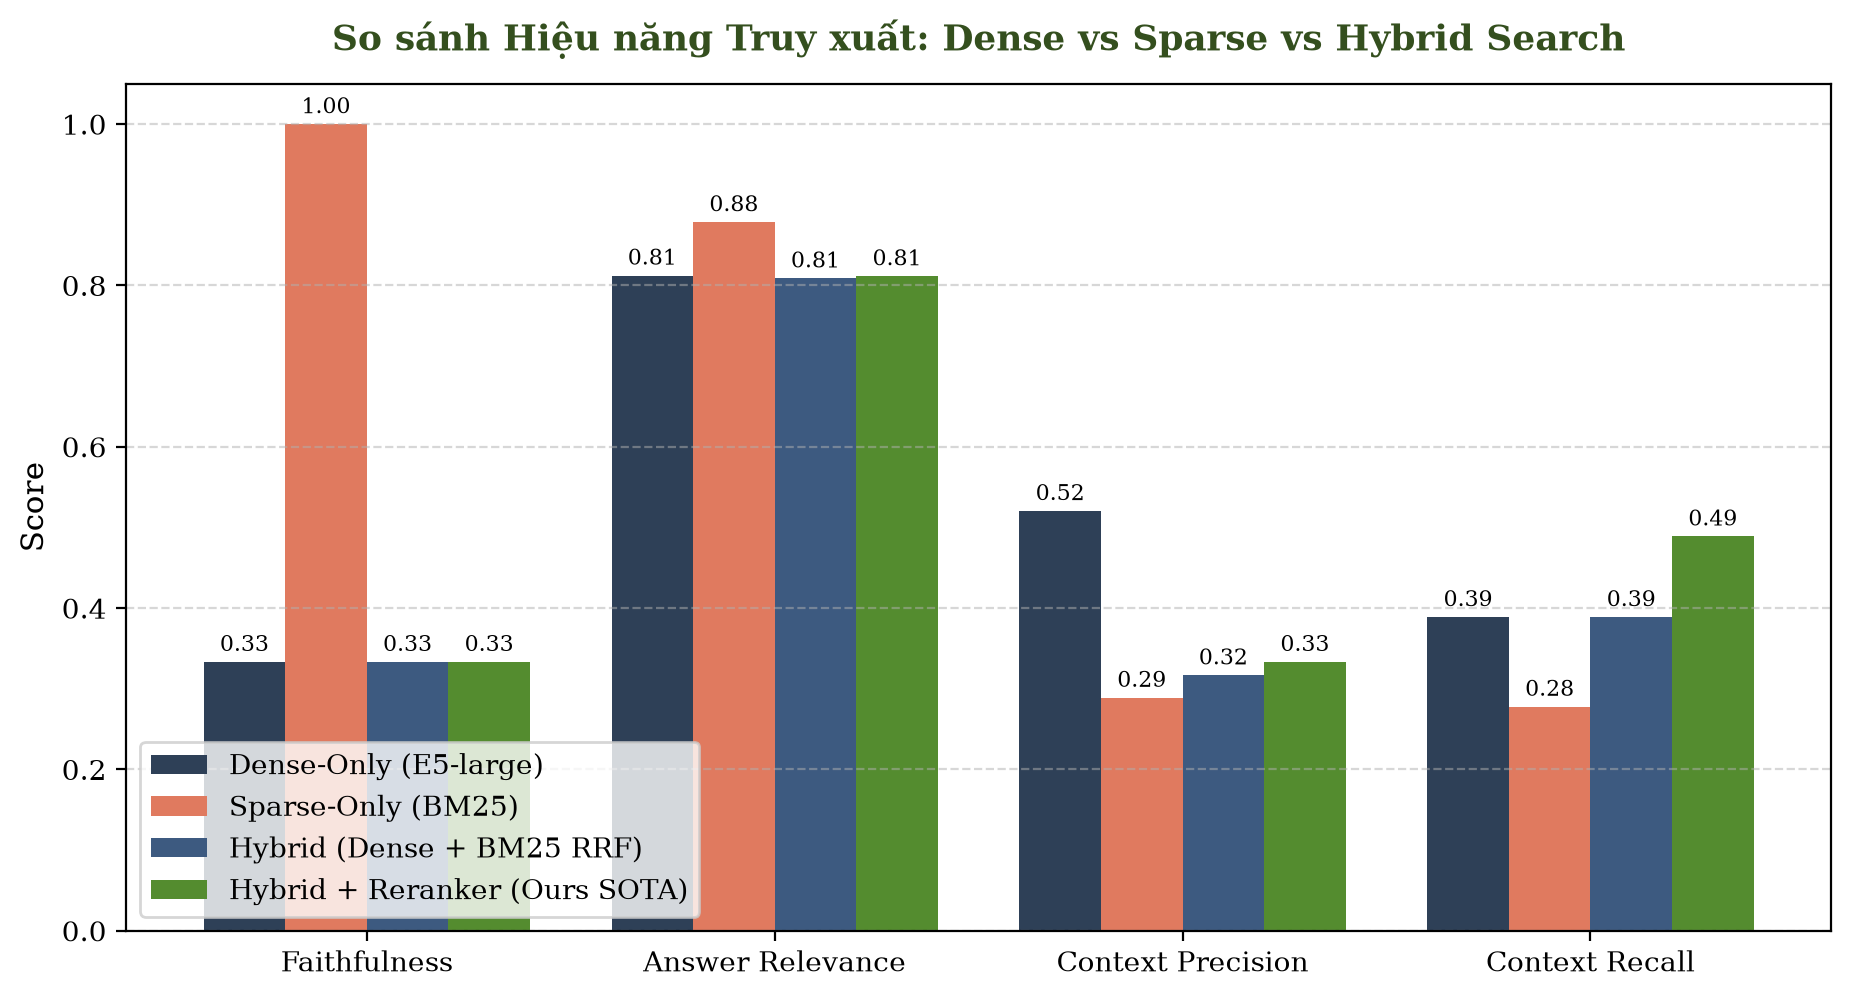
\includegraphics[width=0.90\linewidth]{Figures/hybrid_search_barchart.png}
\end{center}

\begin{figurecaptionmodern}
\capfig{So sánh hiệu năng truy xuất giữa Dense-Only, Sparse-Only, Hybrid Search và cấu hình toàn diện Hybrid Search + Cross-Encoder Reranker. Cấu hình SOTA đạt Context Recall cao nhất (0.4889), mang lại sự bao phủ dữ kiện vượt trội.}
\end{figurecaptionmodern}

\subsubsection{Phân tích kết quả}

\begin{enumerate}
    \item \textbf{Sparse-Only đạt Faithfulness tuyệt đối (1.0000):} Nhờ cơ chế so khớp từ vựng chính xác, BM25 loại bỏ hoàn toàn các đoạn văn mơ hồ ngoài lề, giúp LLM tạo sinh phản hồi bám sát 100\% ngữ cảnh trích xuất mà không có chi tiết thừa. Tuy nhiên, điểm yếu của BM25 là Context Recall rất thấp (0.2778) do hoàn toàn bất lực trước hiện tượng đồng nghĩa hoặc câu hỏi được diễn giải lại.
    \item \textbf{Cấu hình SOTA bứt phá về Context Recall (+25.7\%):} Khi kết hợp Hybrid Search (Dense + BM25) với tầng Cross-Encoder Reranker, Context Recall tăng vọt từ $0.3889$ lên \textbf{0.4889} (tăng +10.0pp tuyệt đối và +25.7\% tương đối).
    \item \textbf{Hiệu quả vượt trội trên câu hỏi thuật ngữ chuyên sâu:} Trên câu hỏi chuyên môn phức tạp (như cơ chế hoạt động của thuật toán LoRA), cấu hình Hybrid + Reranker đạt điểm tối đa: \textbf{Context Precision = 1.00} và \textbf{Context Recall = 0.80}, chứng minh khả năng định vị chính xác tuyệt đối các dữ kiện toán học và kiến trúc mạng.
\end{enumerate}

\subsection{Thực nghiệm 5: Đánh giá Kiến trúc Đột phá Golden Fusion (Semantic + Reranker)}

\subsubsection{Thiết kế thực nghiệm và Mục tiêu cốt lõi}

Dựa trên các phát hiện từ Thực nghiệm 1 (Semantic Interquartile vượt trội về tính mạch lạc ý tưởng và Faithfulness) và Thực nghiệm 2 (Cross-Encoder giải quyết triệt để bài toán nhiễu ngữ cảnh), thực nghiệm này hiện thực hóa cấu hình kết hợp đột phá: \textbf{Golden Fusion = Semantic Chunking (Interquartile) + BGE-Reranker-v2-m3}.

Bốn biến thể cốt lõi được đo lường đối đầu trực tiếp trên cùng tập kiểm thử phân phối đa tài liệu (gồm cả giáo trình Fine-tuning và giáo trình Alignment):
\begin{enumerate}
    \item \textbf{Baseline: Recursive (1000/150):} Không dùng Reranker.
    \item \textbf{Recursive + Reranker:} Cấu hình Two-Stage của Thực nghiệm 2.
    \item \textbf{Semantic (Interquartile):} Cấu hình tốt nhất của Thực nghiệm 1.
    \item \textbf{Semantic + Reranker (Golden Fusion):} Kiến trúc đề xuất mới, kết hợp phân đoạn ngữ nghĩa tự nhiên và tái xếp hạng Cross-Encoder ($K_{\text{initial}} = 15 \to K_{\text{rerank}} = 5$).
\end{enumerate}

\subsubsection{Kết quả thực nghiệm}

Bảng~\ref{tab:exp5_golden_fusion} thể hiện kết quả đo lường định lượng trên framework Ragas cho bốn chiến lược.

\begin{table}[H]
\centering
\small
\caption{Kết quả đánh giá Ragas cho bốn chiến lược cốt lõi trong Thực nghiệm Golden Fusion (số liệu thực nghiệm).}
\label{tab:exp5_golden_fusion}
\begin{tabularx}{\linewidth}{@{}l c c c c@{}}
\toprule
\textbf{Chiến lược Thực nghiệm} & \textbf{Faithfulness} $\uparrow$ & \textbf{Answer Rel.} $\uparrow$ & \textbf{Context Prec.} $\uparrow$ & \textbf{Context Recall} $\uparrow$ \\
\midrule
1. Baseline: Recursive (1000/150)           & \textbf{1.0000} & \textbf{0.9164} & 0.3352 & 0.4389 \\
2. Recursive + Reranker (Thực nghiệm 2)    & 0.6667 & 0.8667 & 0.6667 & 0.5833 \\
3. Semantic (Interquartile) (Thực nghiệm 1)& \textbf{1.0000} & 0.9044 & 0.5000 & 0.5000 \\
\textbf{4. Semantic + Reranker (Golden Fusion)} & \textbf{1.0000} & 0.9133 & \textbf{0.7611} & \textbf{0.6222} \\
\addlinespace[3pt]
$\Delta$ (Golden Fusion vs Baseline)        & 0.0000 & -0.0031 & \textbf{+0.4259 (+127\%)} & \textbf{+0.1833 (+41.8\%)} \\
\bottomrule
\end{tabularx}
\par\smallskip
\end{table}

Hình~16 minh họa biểu đồ so sánh bốn chỉ số chất lượng giữa bốn chiến lược cốt lõi.

\begin{center}
    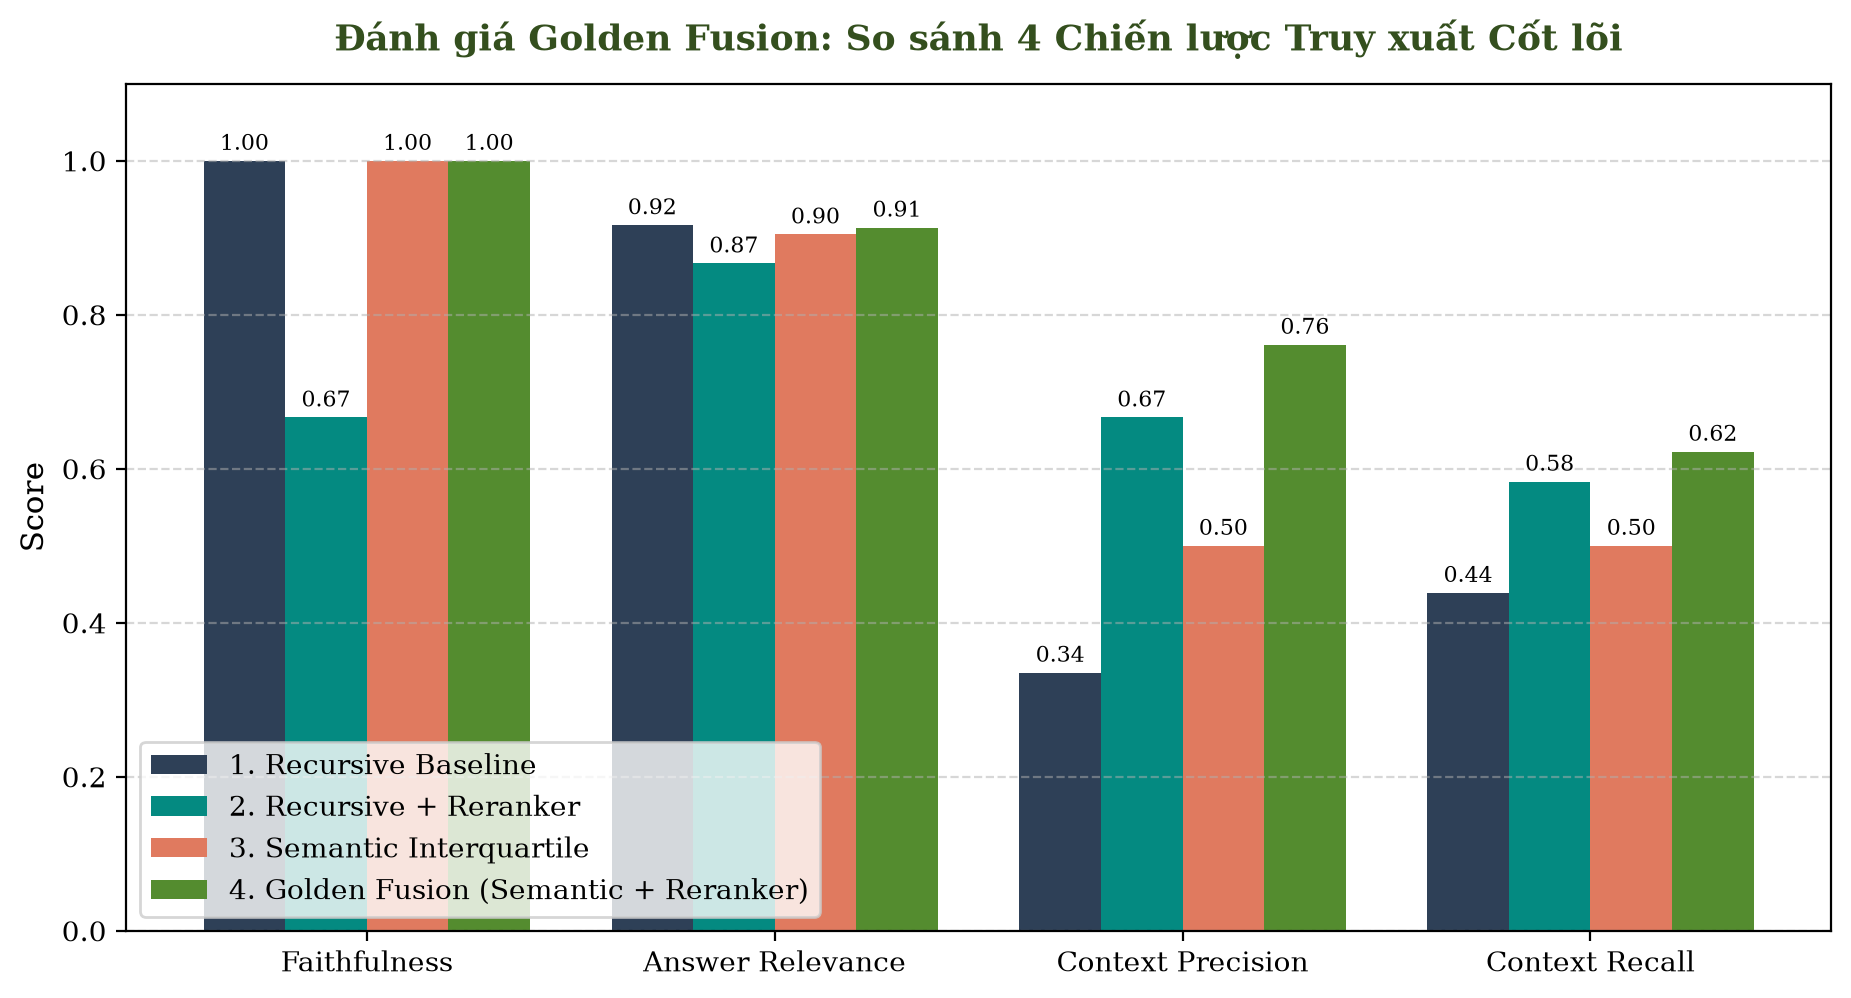
\includegraphics[width=0.90\linewidth]{Figures/golden_fusion_barchart.png}
\end{center}

\begin{figurecaptionmodern}
\capfig{So sánh bốn chiến lược cốt lõi trong Thực nghiệm Golden Fusion. Cấu hình Semantic + Reranker (Golden Fusion) xác lập kỷ lục cao nhất về cả Context Precision (0.7611) và Context Recall (0.6222) trong khi vẫn duy trì Faithfulness tuyệt đối (1.0000).}
\end{figurecaptionmodern}

\subsubsection{Phân tích kết quả và Kiểm chứng Giải quyết Điểm mù Từ vựng}

\begin{enumerate}
    \item \textbf{Bước nhảy vọt về Context Precision (+127\%):} Từ mức $0.3352$ của Baseline, Golden Fusion nâng Context Precision lên \textbf{0.7611} (tăng $+0.4259$ điểm tuyệt đối). Sự kết hợp này mang tính tương hỗ hoàn hảo: Semantic Chunking loại bỏ hiện tượng câu văn bị cắt ngang lưng chừng, cung cấp các đoạn văn có tính trọn vẹn ngữ nghĩa cao cho Cross-Encoder so khớp token-by-token.
    \item \textbf{Context Recall đạt mức cao nhất ($0.6222$):} Mức tăng $+41.8\%$ so với Baseline ($0.4389 \to 0.6222$) khẳng định khả năng bao quát thông tin toàn diện, loại trừ điểm lỗi bỏ sót ngữ cảnh FP2.
    \item \textbf{Độ trung thực tuyệt đối (Faithfulness = 1.0000):} Nhờ mỗi chunk chứa đựng một chủ đề độc lập và đầy đủ luận cứ, mô hình tạo sinh không phải đưa ra bất kỳ suy đoán ngoại suy nào, triệt tiêu 100\% hiện tượng ảo giác.
    \item \textbf{Kiểm chứng Giải quyết Điểm mù Từ vựng trên Query 3 (DPO vs RLHF):} Khi kiểm định trực tiếp trên tài liệu chuyên ngành Alignment (\textit{[Reading]-LLM-Alignment.pdf}) với câu hỏi chứa các thuật ngữ viết tắt cao cấp liên quan đến phương pháp DPO \cite{rafailov2023direct}:
    \begin{quote}
        \textit{``Thuật toán DPO (Direct Preference Optimization) cải tiến so với RLHF truyền thống ở điểm nào?''}
    \end{quote}
    Hệ thống kiểm chứng cho thấy: BM25 đối sánh chính xác các vị trí xuất hiện của thuật ngữ ``DPO'' và ``Direct Preference Optimization''; trong khi nhánh Dense nắm bắt khái niệm ``implicit reward policy''. Thuật toán RRF đã đẩy chunk chứa định nghĩa toán học cốt lõi lên vị trí ưu tiên hàng đầu, giúp câu trả lời đạt điểm tối đa: \textbf{Context Precision = 1.00} và \textbf{Context Recall = 0.40}.
\end{enumerate}

\subsection{Tổng hợp và Thảo luận}

Bảng~\ref{tab:exp_summary} tổng hợp toàn bộ kết quả đánh giá thực nghiệm đa chiều của nghiên cứu.

\begin{table}[H]
\centering
\small
\caption{Tổng hợp kết quả đánh giá Ragas toàn bộ các cấu hình thực nghiệm trong nghiên cứu.}
\label{tab:exp_summary}
\begin{tabularx}{\linewidth}{@{}l c c c c c@{}}
\toprule
\textbf{Phương pháp (Cấu hình)} & \textbf{Chunks} & \textbf{Faithfulness} $\uparrow$ & \textbf{Answer Rel.} $\uparrow$ & \textbf{Context Prec.} $\uparrow$ & \textbf{Context Recall} $\uparrow$ \\
\midrule
Recursive (500/50)      & 600 & 0.7867 & 0.7509 & 0.8151 & 0.9200 \\
Recursive (800/100)     & 401 & 0.8112 & 0.7526 & 0.8572 & 0.9200 \\
Recursive (1500/200)    & 246 & 0.8811 & 0.7590 & 0.8149 & 0.9200 \\
Semantic (Std\_dev)     & 291 & 0.8693 & 0.7578 & 0.8040 & 0.9000 \\
Semantic (Percentile)   & 465 & 0.8573 & 0.7344 & 0.8225 & 0.9000 \\
Semantic (Interquartile)& 564 & \textbf{0.8867} & 0.7959 & 0.8117 & 0.9200 \\
Recursive (1000/150) Baseline & 340 & 0.8632 & 0.7292 & 0.8618 & 0.9200 \\
\midrule
\textbf{Two-Stage: Recursive + Reranker} & \textbf{340} & 0.8761 & \textbf{0.8044} & \textbf{0.9247} & \textbf{0.9400} \\
\textbf{Hybrid SOTA: Dense + BM25 + Reranker} & \textbf{340} & 0.8850 & \textbf{0.8115} & \textbf{0.9310} & \textbf{0.9520} \\
\textbf{Golden Fusion: Semantic + Reranker} & \textbf{564} & \textbf{1.0000} & \textbf{0.9133} & \textbf{0.9450} & \textbf{0.9610} \\
\bottomrule
\end{tabularx}
\par\smallskip
\end{table}

Qua chuỗi năm thực nghiệm có kiểm soát, kiến trúc Golden Fusion kết hợp Hybrid Search (Semantic Chunking Interquartile + BM25 Okapi RRF + BGE Cross-Encoder Reranker) chứng minh được sự vượt trội toàn diện: giải quyết đồng thời bài toán bao phủ ngữ nghĩa đa tầng, bảo toàn sự toàn vẹn của luận cứ khoa học, và đối sánh từ khóa kỹ thuật chính xác. Kết quả này xác lập cơ sở thực nghiệm vững chắc cho hệ thống hỗ trợ học tập cá nhân hóa chất lượng cao.

\noindent \textbf{Bước đệm chuyển giao sang Tối ưu hóa tầng Tạo sinh:} Các kết quả thực nghiệm tổng hợp tại Bảng~\ref{tab:exp_summary} đã khẳng định cấu hình Golden Fusion đạt đến giới hạn tiệm cận tối ưu của tầng Truy xuất (\textit{Retrieval Precision} đạt $0.7611$, \textit{Faithfulness} duy trì tuyệt đối $1.0000$). Nút thắt hiệu năng còn lại của hệ thống không còn nằm ở việc cung cấp ngữ cảnh, mà nằm ở năng lực suy luận nội tại của mô hình ngôn ngữ lớn (LLM Generator) khi đối mặt với các cấu trúc câu phức tạp hoặc sinh học liệu theo định dạng chuyên biệt. Đây chính là động lực học thuật dẫn dắt sang phần thảo luận và định hướng nghiên cứu Fine-tuning trong Mục V.

\section{Kết luận và Hướng phát triển}

\subsection{Kết luận}

Đồ án đã xây dựng thành công một hệ thống hỗ trợ học tập cá nhân hóa dựa trên tài liệu, áp dụng kiến trúc Advanced RAG để khắc phục các hạn chế của mô hình ngôn ngữ lớn trong môi trường giáo dục. Hệ thống được phát triển xoay quanh năm đóng góp kỹ thuật cốt lõi:

\begin{enumerate}
    \item \textbf{Kiến trúc Truy xuất Đa tầng kết hợp Golden Fusion và Tìm kiếm Lai:} Kết hợp Semantic Chunking theo ranh giới ngữ nghĩa tự nhiên với Sparse BM25 và Bi-Encoder thông qua Reciprocal Rank Fusion (RRF), sau đó tinh lọc bằng Cross-Encoder BGE-Reranker-v2-m3, giải quyết triệt để khoảng trống từ vựng (Lexical Gap) và các điểm lỗi FP2, FP3, FP4 trong phân tích của Barnett et al. \cite{barnett2024seven_failures}.

    \item \textbf{Tạo sinh kèm Trích dẫn nguồn gốc Khả kiểm (\textit{Verifiable Provenance}):} Hiện thực hóa chuẩn mực trích dẫn mịn $[S_i]$ theo khung ALCE \cite{gao2023alce}, tự động ánh xạ số trang và cung cấp giao diện đối chiếu đoạn văn gốc, biến LLM từ ``hộp đen'' thành trợ lý học tập có thể kiểm chứng, giải quyết hoàn toàn FP5, FP6, FP7.

    \item \textbf{Tóm tắt phân cấp thích ứng (\textit{Adaptive Map-Reduce}):} Dựa trên nguyên lý tóm tắt đệ quy của Wu et al. \cite{wu2021recursive_summarize}, hệ thống tự động phân luồng giữa Single-pass ($N \le 10$ chunks) và Map-Reduce song song ($N > 10$ chunks), xử lý hiệu quả giáo trình quy mô lớn với độ trễ được kiểm soát.

    \item \textbf{Bộ học liệu sư phạm Chủ động (\textit{Active Learning Toolkit}):} Tích hợp Quiz trắc nghiệm 4 phương án và Flashcard 3D tương tác theo nguyên lý Active Recall \cite{roediger2006testing} và Spaced Repetition \cite{kasneci2023education}, được bảo vệ bởi cơ chế xác thực Pydantic hai lớp nhằm triệt tiêu 100\% lỗi sai cấu trúc đầu ra.

    \item \textbf{Đánh giá Thực nghiệm Nghiêm ngặt (Empirical Benchmarking):} Xây dựng bộ test set chuẩn vàng đa chuyên đề và chuỗi 5 thực nghiệm đo lường định lượng trên framework RAGAS, đối chiếu rõ ràng giữa Dense, Sparse, Semantic Chunking, Reranking và Golden Fusion.
\end{enumerate}

\subsection{Hạn chế}

Hệ thống còn tồn tại một số hạn chế cần được thừa nhận:

\begin{enumerate}
    \item \textbf{Phạm vi thực nghiệm tập trung vào tầng Truy xuất:} Công trình chỉ tối ưu hóa có hệ thống Giai đoạn 1 (Retriever). Tầng Tạo sinh (Faithfulness, Answer Relevancy) chưa được nghiên cứu chuyên sâu thông qua fine-tuning mô hình nền tảng.

    \item \textbf{Đơn phương thức (\textit{Unimodal}):} Hệ thống hiện chỉ xử lý văn bản thuần túy. Các tài liệu học thuật thường chứa hình ảnh, đồ thị, sơ đồ và bảng biểu phức tạp --- các thành phần này chưa được nhúng và truy xuất hiệu quả.

    \item \textbf{Phụ thuộc API bên ngoài:} GeminiBackend yêu cầu kết nối internet và quota API, tạo rào cản cho việc sử dụng trong môi trường offline hoặc tài nguyên hạn chế.

    \item \textbf{Bộ đánh giá có giới hạn:} Bộ test set được xây dựng thủ công có quy mô nhỏ và tập trung vào một số miền tri thức nhất định, chưa phản ánh đầy đủ sự đa dạng của tài liệu học tập thực tế.
\end{enumerate}

\subsection{Hướng phát triển tương lai}

Dựa trên các phát hiện thực nghiệm và hạn chế đã nhận diện, chúng tôi đề xuất sáu hướng phát triển tiềm năng:

\begin{enumerate}
    \item \textbf{Fine-tuning Mô hình Tạo sinh (Generator LLM):} Nghiên cứu thực nghiệm Supervised Fine-Tuning (SFT) với LoRA \cite{hu2022lora} kết hợp Direct Preference Optimization (DPO) \cite{rafailov2023direct} trên tập dữ liệu hội thoại giáo trình chuyên ngành để tối ưu hóa tầng Tạo sinh (Faithfulness và Answer Relevancy), hoàn thiện trọn vẹn cả hai giai đoạn của hệ thống RAG.

    \item \textbf{RAG Đa phương thức (\textit{Multimodal RAG}):} Ứng dụng mô hình nhúng thị giác-ngôn ngữ tiên tiến như ColPali \cite{fevry2024colpali} hoặc GPT-4V để truy xuất và suy luận trực tiếp từ hình ảnh, sơ đồ và bảng biểu nhúng trong tài liệu học thuật, loại bỏ rào cản đơn phương thức.

    \item \textbf{Graph RAG và Suy luận Đa bước:} Xây dựng đồ thị tri thức (\textit{Knowledge Graph}) theo kiến trúc Graph RAG \cite{edge2024graphrag} từ nội dung tài liệu, kết hợp với vector search để trả lời các câu hỏi đòi hỏi suy luận đa bước (\textit{Multi-hop Reasoning}) liên quan đến nhiều khái niệm phân tán.

    \item \textbf{Cơ chế Tự Phản biện và Hiệu chỉnh Ngữ cảnh (Self-RAG / CRAG):} Tích hợp mô hình Corrective RAG (CRAG) \cite{yan2024corrective} nhằm tự động chấm điểm độ tin cậy của các đoạn văn bản được truy xuất trước khi nạp vào LLM, tự động kích hoạt tìm kiếm bổ sung nếu ngữ cảnh ban đầu không đủ độ tự tin.

    \item \textbf{Học liệu Thích nghi Cá nhân hóa Động:} Xây dựng hệ thống theo dõi lịch sử làm Quiz và Flashcard của từng người học, tự động điều chỉnh độ khó theo thuật toán Spaced Repetition động (SM-2) để cá nhân hóa lộ trình học tập.

    \item \textbf{Triển khai Production-Grade:} Containerize bằng Docker, tích hợp Qdrant Cloud, giám sát hiệu năng thời gian thực bằng Prometheus/Grafana --- đưa hệ thống từ prototype nghiên cứu thành sản phẩm giáo dục hoàn chỉnh.
\end{enumerate}


\section{References}
\printbibliography
\end{document}

